\documentclass[a4paper,11pt]{article}
\usepackage[T1]{fontenc}
\usepackage[margin=1in]{geometry}
\usepackage{amsmath,amssymb,graphicx,booktabs}
\usepackage[hidelinks]{hyperref}
\graphicspath{{graphs/}}
% Canonical graph references use EPS. PDF engines read the supplied vector PDF
% companions, exported from the identical figure, without an external converter.
% A latex -> dvips workflow uses the EPS sources directly.
\newif\ifProjectPDF
\ifdefined\XeTeXversion
  \ProjectPDFtrue
\else
  \ifdefined\pdfoutput
    \ifnum\pdfoutput>0
      \ProjectPDFtrue
    \fi
  \fi
\fi
\makeatletter
\newcommand{\ReportGraphEPS}[2][]{%
  \IfFileExists{graphs/#2}{}{\PackageError{project}{Missing required EPS source #2}{Include every EPS graph in graphs/}}%
  \begingroup
  \filename@parse{#2}%
  \ifProjectPDF
    \edef\ProjectGraphFile{\filename@area\filename@base.pdf}%
  \else
    \def\ProjectGraphFile{#2}%
  \fi
  \includegraphics[#1]{\ProjectGraphFile}%
  \endgroup
}
\makeatother
\setcounter{topnumber}{5}
\setcounter{bottomnumber}{5}
\setcounter{totalnumber}{5}
\renewcommand{\topfraction}{0.95}
\renewcommand{\bottomfraction}{0.95}
\renewcommand{\textfraction}{0.05}
\renewcommand{\floatpagefraction}{0.7}
\setlength{\floatsep}{12pt}
\setlength{\textfloatsep}{12pt}
\makeatletter
\setlength{\@fptop}{0pt}
\setlength{\@fpsep}{12pt}
\setlength{\@fpbot}{0pt plus 1fil}
\makeatother

\usepackage{amsthm,array,tabularx}
\setlength{\emergencystretch}{2em}
\newtheorem{theorem}{Theorem}
\newtheorem{proposition}{Proposition}
\newtheorem{lemma}{Lemma}
\theoremstyle{remark}\newtheorem{remark}{Remark}
\title{Lynx and Hare Dynamics\\Model, Stability, Numerical Simulation and Inverse Inference}
\author{Arnav \and Joel \and Rishi \and Yash \and Advay}
\date{28 October 2026}
\begin{document}\maketitle
\begin{abstract}
We combine a Rosenzweig--MacArthur model, equilibrium and Hopf analysis, numerical
experiments, and historical parameter fitting using least squares and an inverse PINN.
The Stan pelt-index compilation is split into 1900--1915 training and 1916--1920
evaluation. Primary held-out RMSE is 3.07/3.04 thousand pelts for least squares and
2.85/4.32 for the PINN-derived ODE (hare/lynx). The comparison is mixed; observation-model
and bound sensitivity prevent precise biological recovery or a robust ecological
limit-cycle claim. Frozen numerical evidence, sources and all sensitivity variants
are retained. No final integration step retunes a model using test-year errors.
\end{abstract}
\paragraph{Contributions and evaluation chronology.}
Arnav: model and units. Joel: theory. Rishi: numerical validation. Yash: PINN and
integration. Advay: data and independent least squares/evaluation. Historical forecasts
use the same dimensional RHS and solver configuration. Advay's independent reproduction
followed Yash's published scored iteration, so it is not a new blinded test. Training
demonstrations in the combined notebook do not overwrite the frozen forecasts.
\tableofcontents\clearpage
% Integration copy; canonical source: contributions/arnav/sections/arnav_model.tex
\section{Problem and observation convention}
The project asks whether a mechanistic predator--prey model can explain recurring
hare--lynx fluctuations and support useful predictions beyond the observations used
for calibration. This section establishes the equations, their biological assumptions,
units and dimensionless form. It supplies the common mathematical foundation for the
team's stability analysis, numerical simulations and parameter estimation.

The completed historical iteration uses annual observations labelled 1900--1920.
The Stan case study supplies a public transcription of Hudson's Bay Company pelt
records in thousands of pelts, with a documented source chain
\cite{arnav_carpenter2018}. These measurements are trade records, not population
censuses. We interpret $H(t)$ and $P(t)$ as nonnegative hare and lynx abundance
\emph{indices}, respectively, in explicitly declared species-specific units.
The comparison between a continuous state and an annual pelt total is an observation
approximation: trapping effort, capture probability, seasonal aggregation and
unmodelled ecology can all affect the relationship.

Advay's frozen data split and the reference configuration use one index unit per
thousand pelts for each species \cite{arnav_advay2026,arnav_historical2026}.
The Stan compilation remains the source for this iteration. The alternative
tsibbledata compilation disagrees with it, a documented source limitation; neither
series establishes absolute animal abundance, and they are not combined.
Set $t=\mathrm{Year}-1900$ in years. The implemented evaluation design uses
1900--1915 for calibration and 1916--1920 for final scoring. Normalization and
parameter selection use training observations only. Forecasts have already been
frozen and scored; this section documents their observation convention without
changing it. It does not provide additional historical fits.

\subsection{Explicit observation model}
For year $\mathrm{Year}_i$ and $t_i=\mathrm{Year}_i-1900$, write
\begin{equation}\label{eq:arnav_observation}
Y_{H,i}=H(t_i)+\varepsilon_{H,i},\qquad
Y_{P,i}=P(t_i)+\varepsilon_{P,i}.
\end{equation}
Here $Y$ is the recorded annual pelt count in thousands; $H,P$ are the model's
noiseless pelt indices; and $\varepsilon$ is observation discrepancy in the same
species-specific units. Under the working proportional-index assumption O1,
\begin{equation}\label{eq:arnav_O1}
H(t)=c_H N_H(t),\qquad P(t)=c_P N_P(t),\qquad c_H,c_P>0,
\end{equation}
where $N_H,N_P$ denote latent animal abundance and the unknown observation factors
are constant. We fit the effective equations directly in pelt units:
\emph{no observation-scale factor is fitted}. This does not set $c_H=c_P=1$ or
identify actual animal counts. Constant factors are absorbed into the effective
coefficients through the transformation derived in Eq.~\eqref{eq:arnav_unitmap}.

Each annual total is approximated by a point observation of the state, as in the
implemented convention \cite{arnav_advay2026,arnav_historical2026}. Thus $H,P$ have
units of thousands of pelts, and $\dot H,\dot P$ have units of thousands of pelts
per year. No seasonal observation integral is fitted. A latent-population model
with estimated observation factors, or an integral over the trapping season,
would represent additional mechanisms but require further assumptions and
unknowns. O1 and the point-sample approximation keep the present comparison
tractable, at the cost of limited biological interpretation.

The main observation loss compares additive residuals after division by the
training maxima $s_H=77.4$ and $s_P=59.4$:
\begin{equation}\label{eq:arnav_obsresidual}
R_{H,i}=\frac{H(t_i)-Y_{H,i}}{s_H},\qquad
R_{P,i}=\frac{P(t_i)-Y_{P,i}}{s_P}.
\end{equation}
For the PINN data term the state in this expression is the network approximation;
for least squares it is the integrated ODE state. Both methods use the same
species scales. These weights are a declared comparison convention, not measured
noise standard deviations. Additive discrepancy notation alone establishes
neither Gaussian noise nor independence of observations. The reported log-error
sensitivity instead emphasizes relative discrepancies. A separate sensitivity
fits the 1900 initial states within $[0.5,1.5]$ times their observed values
\cite{arnav_historical2026}; the two checks change different assumptions and
remain separate outcomes.

\section{From Lotka--Volterra to the chosen model}
\subsection{The reference model and its limitation}
For a first comparison, let
\begin{equation}\label{eq:arnav_lv}
\dot H=rH-cHP,\qquad \dot P=ecHP-mP,
\end{equation}
where a dot means differentiation with respect to years. The prey grows at rate
$rH$ without predators, encounters remove prey at rate $cHP$, conversion of consumed
prey contributes $ecHP$ to predator growth, and predator mortality removes $mP$.
Here $c>0$ is the encounter coefficient; it is not the saturation parameter $a$
introduced below. The other parameters are positive.

The positive equilibrium is $H_*=m/(ec)$, $P_*=r/c$. To see why the cycles are
neutral, rather than simply asserting it, define for positive $H,P$
\begin{equation}
V=ec\left[H-H_*-H_*\log(H/H_*)\right]
 +c\left[P-P_*-P_*\log(P/P_*)\right].
\end{equation}
The logarithms have dimensionless arguments. Differentiation gives
\begin{align}
\dot V&=(ec-m/H)\dot H+(c-r/P)\dot P\\
&=(ecH-m)(r-cP)+(cP-r)(ecH-m)=0.
\end{align}
Each bracket in $V$ has a strict minimum at its equilibrium value and diverges at
zero or infinity. Thus nonzero level sets are closed curves in the positive
quadrant, surrounding the equilibrium. The vector field has no other positive
equilibrium on a level set, so trajectories follow periodic orbits. A perturbation
generally moves the state to a different orbit; it does not relax back to one
selected cycle. The equilibrium is a centre, not an attractor. Also, predator-free
prey grows exponentially without a resource limit. These are reasons to refine the
model; they do not mean that Lotka--Volterra cannot oscillate.

\subsection{Resource limitation and saturating predation}
Let the prey's per-capita net growth decrease linearly from $r$ at low abundance
to zero at $H=K$. Multiplication by $H$ gives logistic growth,
\begin{equation}
G(H)=rH(1-H/K).
\end{equation}
The carrying capacity $K$ describes the prey-only resource limit under fixed
environmental conditions; it is not an absolute ceiling on every trajectory.

Let $g(H)$ be consumption per predator. A simple search-and-handling argument
assumes an encounter-limited rate $qH$ while searching and a maximum processing
rate $a$. If the fractions of time searching and handling are $g/(qH)$ and $g/a$,
their sum is one. For $H>0$,
\begin{equation}
\frac{g}{qH}+\frac{g}{a}=1
\quad\Longrightarrow\quad
g(H)=\frac{aqH}{a+qH}=\frac{aH}{b+H},\qquad b=\frac{a}{q}.
\end{equation}
Extend continuously by $g(0)=0$. This is the Holling type II response
\cite{arnav_holling1959}. It assumes an effectively constant prey level over the
short feeding interval and no predator interference. In index units it is an
effective response law, not a direct measurement of handling time. The parameters
have transparent interpretations:
\begin{equation}
g(b)=a/2,\qquad \lim_{H\to\infty}g(H)=a,\qquad
g(H)\simeq(a/b)H\quad\text{when }H/b\ll1.
\end{equation}
The auxiliary $q=a/b$ has units inverse lynx index per year. It is not an additional
parameter to estimate. The linear response would be simpler but cannot represent
saturation; a type III response would introduce a different low-prey mechanism
that the present project does not establish.

\subsection{Dimensional Rosenzweig--MacArthur equations}
Combining logistic growth, total prey consumption $g(H)P$, conversion and mortality
gives the project's Rosenzweig--MacArthur model
\cite{arnav_rosenzweig1963}:
\begin{align}
\frac{dH}{dt}&=rH\left(1-\frac{H}{K}\right)-\frac{aHP}{b+H},\label{eq:arnav_H}\\
\frac{dP}{dt}&=\frac{eaHP}{b+H}-mP.\label{eq:arnav_P}
\end{align}
These are exactly the dimensional equations in the shared repository
\cite{arnav_teamrepo2026}. Logistic
growth and saturation allow stability to depend on parameters. Whether a specified
case approaches an equilibrium or exhibits a stable cycle requires the subsequent
analysis and numerical evidence; it does not follow merely from naming the model.

\section{Units and assumptions}
Let $U_H$ and $U_P$ denote the chosen hare and lynx index units. Keeping these labels
distinct prevents an unjustified interpretation of conversion efficiency.
\begin{center}
\small
\begin{tabularx}{\linewidth}{@{}lXl@{}}
\toprule
Symbol & Meaning & Units\\\midrule
$t$ & Elapsed time & year\\
$H$, $P$ & Hare and lynx states & $U_H$, $U_P$\\
$r$ & Low-density hare net growth rate & year$^{-1}$\\
$K$ & Effective prey-only carrying-capacity index & $U_H$\\
$a$ & Effective saturated consumption coefficient & $U_H U_P^{-1}$ year$^{-1}$\\
$b$ & Prey index at half saturation & $U_H$\\
$e$ & Effective predator conversion coefficient & $U_P U_H^{-1}$\\
$m$ & Predator mortality rate & year$^{-1}$\\
$H_0$, $P_0$ & States at the initial time & $U_H$, $U_P$\\
\bottomrule
\end{tabularx}
\end{center}
All six parameters are strictly positive. For example,
$[aHP/(b+H)]=U_H$/year and $[eaHP/(b+H)]=U_P$/year, matching the two left-hand
sides. In separately scaled abundance indices, $e$ is an effective conversion
factor. It need not be a dimensionless biomass efficiency bounded above by one.
For this historical iteration $U_H$ means thousands of hare pelts and $U_P$
thousands of lynx pelts. The rates $r,m$ retain their growth/mortality interpretation
only conditional on O1 and an adequate dynamical model; $K,b,a,e$ are effective
pelt-unit coefficients. Scale invariance does not establish accurate recovery of
any biological parameter.

The simplifying assumptions and their consequences are:
\begin{enumerate}
\item A closed two-species system has no immigration, emigration, alternative prey
or other predators. This isolates the proposed feedback but omits a food web.
\item Continuous, spatially mixed states omit age structure, territories and local
differences. The approximation is unsuitable for individual-level extinction claims.
\item Constant parameters omit seasons, weather and changing resource availability.
Fitted rates summarize the chosen interval rather than universal ecological constants.
\item Resource limitation is represented by logistic prey growth. Plants are not
modelled as a third dynamical state.
\item Predation follows the type II response with no interference between predators.
Predator growth depends on prey; without prey, $P$ decays at rate $m$.
\item Pelt totals are treated as noisy abundance proxies. Constant observation
scales are a working assumption. Unknown or changing capture rates can confound
parameter inference. Harvest is not modelled as an additional removal process.
\end{enumerate}

\subsection{Basic consistency checks}
The equations have the form $\dot H=H A(H,P)$, $\dot P=P B(H)$ with continuous
coefficients for $H\geq0$. Along a finite solution interval,
\begin{equation}
H(t)=H_0\exp\!\left(\int_0^t A(H(s),P(s))\,ds\right),\quad
P(t)=P_0\exp\!\left(\int_0^t B(H(s))\,ds\right).
\end{equation}
Positive initial states remain positive, and either zero boundary is invariant by
uniqueness. A numerical method can still introduce negative approximations, so its
outputs must be checked. Also $\dot H\leq rH(1-H/K)$, giving
$H(t)\leq\max\{H_0,K\}$ for $t\geq0$. Since $\dot P\leq eaP$, predator abundance
cannot blow up in finite time. These checks establish basic consistency, not
ecological accuracy or long-term stability.

\section{Non dimensionalisation}
\subsection{Choosing the scales}
For a fixed parameter vector define
\begin{equation}\label{eq:arnav_scales}
s=rt,\qquad x=H/K,\qquad y=\frac{aP}{rK}.
\end{equation}
The corresponding reference time and states are $1/r$, $K$ and $rK/a$.
Their units are year, $U_H$ and $U_P$. The scales therefore make all three new
variables dimensionless. Choosing $K$ for prey makes the prey-only capacity one;
choosing $rK/a$ for predators makes the prey-loss coefficient one. This is the
same notation used in Joel's existing dimensionless analysis
\cite{arnav_joel2026}.

Define the three dimensionless groups
\begin{equation}\label{eq:arnav_groups}
\beta=b/K,\qquad \alpha=ea/r,\qquad \delta=m/r.
\end{equation}
They compare half saturation with carrying capacity, maximum predator growth with
prey growth, and predator mortality with prey growth, respectively. This scaling
also means a sweep of $K$ changes both $\beta$ and the state scales. If the
dimensional initial states are held fixed in that sweep, their scaled values must
be recomputed for each $K$.

\subsection{Substitution and chain rule}
Because $H=Kx$, $P=(rK/a)y$ and $ds/dt=r$,
\begin{equation}
\frac{dH}{dt}=rK\frac{dx}{ds},\qquad
\frac{dP}{dt}=\frac{r^2K}{a}\frac{dy}{ds}.
\end{equation}
Substitution into the prey equation gives
\begin{equation}
rK\frac{dx}{ds}=rKx(1-x)-\frac{rKxy}{b/K+x}.
\end{equation}
Substitution into the predator equation gives
\begin{equation}
\frac{r^2K}{a}\frac{dy}{ds}
=\frac{erKxy}{b/K+x}-\frac{mrK}{a}y.
\end{equation}
Dividing by the respective factors yields
\begin{align}
\frac{dx}{ds}&=x(1-x)-\frac{xy}{\beta+x},\label{eq:arnav_x}\\
\frac{dy}{ds}&=\alpha\frac{xy}{\beta+x}-\delta y.\label{eq:arnav_y}
\end{align}
The two systems describe the same trajectories after the changes of units. Reducing
six dimensional parameters to three groups does not prove that all six can be
identified from data: physical scales and initial conditions also carry information.

\subsection{Initial conditions and conversion back}
At year 1900, $s=0$, $x_0=H_0/K$ and $y_0=aP_0/(rK)$. Recover the dimensional
variables using
\begin{equation}
\mathrm{Year}=1900+s/r,\qquad H=Kx,\qquad P=(rK/a)y.
\end{equation}
If $r,K,a$ are separately specified, recover
$b=\beta K$, $e=\alpha r/a$ and $m=\delta r$. The three dimensionless groups alone
cannot reconstruct all six dimensional parameters.

For an arithmetic check, use the repository's synthetic values
\cite{arnav_teamrepo2026}:
\[
(r,K,a,b,e,m)=(1,60,2,20,0.6,0.5),\qquad (H_0,P_0)=(35,9).
\]
These give
\begin{equation}
(\beta,\alpha,\delta)=(1/3,1.2,0.5),\qquad (x_0,y_0)=(7/12,0.3).
\end{equation}
At this initial state, $(\dot H,\dot P)=(413/132,261/110)$ in their respective
index units per year. The dimensionless derivatives are
$(dx/ds,dy/ds)=(413/7920,87/1100)$; multiplying by $rK=60$ and
$r^2K/a=30$ recovers the dimensional values. These are synthetic checks, not fitted
historical estimates.

An equally valid alternative is $X=H/b=x/\beta$ and $Y=aP/(rb)=y/\beta$,
with the same time $s$. Writing $\kappa=K/b=1/\beta$ gives
$X_s=X(1-X/\kappa)-XY/(1+X)$ and
$Y_s=\alpha XY/(1+X)-\delta Y$. This keeps state scales fixed during a $K$
sweep when other parameters remain fixed. We use the $K$-based form as the main
convention to match the existing team analysis, while retaining the alternative
as an explanation of the scaling tradeoff.

\section{Compatibility with data scaling and the PINN}
\subsection{Keep mathematical and numerical coordinates explicit}
The historical PINN \cite{arnav_historical2026} uses fixed training maxima $s_H,s_P$, normalized outputs
$u=H/s_H$, $v=P/s_P$, training duration $T=15$ years, and internal time input
$\xi=2t/T-1$. It differentiates with respect to elapsed years $t$.
These numerical choices can coexist with the dimensionless theory coordinates.
In elapsed time,
\begin{align}
\frac{du}{dt}&=ru(1-s_Hu/K)-\frac{a s_Puv}{b+s_Hu},\\
\frac{dv}{dt}&=\frac{ea s_Huv}{b+s_Hu}-mv.
\end{align}
The bridge to the theoretical variables is
\begin{equation}
x=(s_H/K)u,\qquad y=\frac{a s_P}{rK}v,\qquad
s=\frac{rT}{2}(\xi+1).
\end{equation}
If differentiation is instead performed with respect to $\xi$, the chain rule
requires $du/dt=(2/T)du/d\xi$, and likewise for $v$. Thus a residual formed in
years is $R_u=(2/T)u_\xi-f_H/s_H$. If one forms a residual in $\xi$ coordinates,
$\widetilde R_u=u_\xi-(T/2)f_H/s_H=(T/2)R_u$. With the same averaging convention,
its squared penalty is $(T/2)^2$ larger; the loss coefficient must be multiplied
by $(2/T)^2$ to preserve the same objective. This is a unit change, not evidence
that one trained model is better.

Because all six coefficients, including $r$ and $a$, are inferred in this iteration, directly using $rt$
and $aP/(rK)$ as fixed training inputs or targets would introduce parameter-dependent
coordinates. Retaining his fixed training normalization avoids that complication.
The dimensionless form is for derivation, interpretation and consistent
mapping, and does not require rewriting the PINN.

\subsection{Why measurement units change parameter meanings}
For any constant positive changes $\widetilde H=c_HH$,
$\widetilde P=c_PP$, keeping time in years preserves the model form if
\begin{equation}\label{eq:arnav_unitmap}
\widetilde r=r,\quad \widetilde m=m,\quad
\widetilde K=c_HK,\quad \widetilde b=c_Hb,\quad
\widetilde a=\frac{c_H}{c_P}a,\quad
\widetilde e=\frac{c_P}{c_H}e.
\end{equation}
This follows by substituting into both derivatives, including the denominator.
It leaves $\beta,\alpha,\delta,x,y$ unchanged. For example, converting both species
from counts to thousands uses $c_H=c_P=10^{-3}$: $K$ and $b$ divide by 1000,
while $a$ and $e$ keep their numerical values. Unequal species scales change
$a$ and $e$ too. Unknown pelt-to-population multipliers have the same algebraic
effect, but their unknown values prevent conversion to absolute biological rates.
Time-varying multipliers would add derivative terms and are outside this model.

The same transformation leaves Joel's stability ratio $\sigma=K/K_H$ unchanged,
where $K_H=b(ea+m)/(ea-m)$ and positive coexistence is applicable
\cite{arnav_joel2026}. Thus the dimensionless groups have a model-based
interpretation independent of constant observation scaling. This does not confirm
that the real ecosystem follows the model or has a stable limit cycle.

With the observed predator scale fixed, an arbitrary rescaling of $P$ cannot
preserve the same observations. Moreover, $a$ occurs separately in the prey
equation while $ea$ occurs in the predator equation. Therefore the scale ambiguity
alone does not prove that effective $a$ and $e$ are inseparable. It also does not
prove that all six coefficients are well determined by 16 annual pairs.

\subsection{Reference settings for the completed iteration}
The reference is \texttt{configs/historical.json}, rather than the earlier
synthetic configuration \cite{arnav_historical2026}. State order is $(H,P)$ and
parameter names are $(r,K,a,b,e,m)$, matching the shared right-hand side.
All six coefficients are fitted. Their independent positive bounds are
\[
r,m\in[0.05,3],\quad K\in[20,500],\quad a\in[0.05,10],\quad
b\in[0.5,300],\quad e\in[0.02,5].
\]
The units are those in the table above. These are exploratory numerical bounds,
not measured ecological ranges. The completed iteration imposes neither $e\leq1$
nor a coexistence constraint. This describes the recorded computation, rather
than a new assertion of identifiability or a proposed change to the inverse problem.

Historical fitting and ODE forecasts use \texttt{model.solve}: RK45 with relative
tolerance $10^{-8}$, absolute tolerance $10^{-10}$ and maximum step $0.1$ years.
Rishi's tighter settings for illustrative long-run simulations are a separate
calculation, not the settings of this historical comparison
\cite{arnav_historical2026,arnav_rishi2026}.

In the main analysis the ODE starts at the observed 1900 index state $(30,4)$.
The PINN enforces its initial state with a soft penalty and reports the discrepancy;
we do not describe this as an exact network constraint. In the fitted-initial-state
sensitivity, each method forecasts from its fitted state at 1900. Every forecast
integrates from 1900 through 1920 with frozen parameters; none restarts from a
test-year observation. The historical handoff records both sensitivity variants
and preserves them alongside the main result \cite{arnav_historical2026}.

\section{Validation responsibilities and limits}
The derivations supply a model to test, not a claim that a published model is novel
or that a PINN earns bonus marks automatically. The independent contribution here
is the explicit reasoning, unit audit, coordinate transformations and interpretation
under the chosen observation convention. The accompanying notebook checks algebraic
equivalence at multiple exact rational inputs. These checks do not replace empirical
validation or establish parameter identifiability.

Joel's contribution supplies equilibrium, stability and Hopf analysis
\cite{arnav_joel2026}; Rishi's supplies numerical checks and parameter-regime
illustrations \cite{arnav_rishi2026}. Advay's data records and Yash's historical
fits, matching least-squares benchmark and evaluation are available
\cite{arnav_advay2026,arnav_historical2026}. Their empirical results belong in the
corresponding report sections. Comparisons use the same training years,
parameter bounds, initial-state convention and solver settings, with separate
hare and lynx MAE and RMSE in thousands of pelts. The PINN's soft initial penalty
and its network--ODE discrepancy must remain visible qualifications.

Five held-out years offer limited evidence. Synthetic recovery generated by the
same equations checks the inverse procedure under favourable assumptions; it is
not independent evidence that those equations describe real ecology. A small
training error does not show unique biological parameters. Any substantive change
after the completed evaluation must be documented as a later revision, preserving
the existing results. Report claims must remain restricted to the mathematical
and empirical evidence actually obtained.
\clearpage
% Integration copy: feasibility/observation-scale qualifications reconciled with Arnav and the frozen protocol.
% =====================================================================
%  Section owner: Joel -- Equilibria, stability and Hopf bifurcation
%  Drop-in file:  % =====================================================================
%  Section owner: Joel -- Equilibria, stability and Hopf bifurcation
%  Drop-in file:  % =====================================================================
%  Section owner: Joel -- Equilibria, stability and Hopf bifurcation
%  Drop-in file:  \input{joel_stability_section}   (standalone build: joel_main.tex)
%  Needs: amsmath, amssymb, amsthm (theorem, proposition, lemma, remark
%         environments), booktabs, graphicx (PDF companions are used under pdflatex)
%  Figures: graphs/joel_{nullclines,trace_det,regions}.{eps,pdf}
%  Regenerate: python scripts/joel_stability_analysis.py
%  Bibliography keys: in report/references.bib
% =====================================================================

\section{Equilibria, Stability and Hopf Bifurcation}\label{sec:joel}

Throughout this section we analyse the dimensional Rosenzweig--MacArthur model
\begin{equation}\label{eq:rm}
\frac{dH}{dt}= f(H,P) = rH\Bigl(1-\frac{H}{K}\Bigr)-\frac{aHP}{b+H},
\qquad
\frac{dP}{dt}= g(H,P) = \frac{eaHP}{b+H}-mP,
\end{equation}
with all six parameters $r,K,a,b,e,m$ strictly positive, as defined in the model section.
Every stability statement below is tied either to a derivation given here, to a
cited theorem, or to a numerical check; Table~\ref{tab:joel-evidence} at the end of the
section records which is which.

% ---------------------------------------------------------------------
\subsection{Well-posedness: invariance and boundedness}

\begin{lemma}\label{lem:bounded}
The closed quadrant $\{H\ge 0,\,P\ge 0\}$, both coordinate axes, and the open quadrant are
invariant under~\eqref{eq:rm}. Every solution starting in the quadrant is bounded, with
\[
\limsup_{t\to\infty} H(t)\le K,
\qquad
\limsup_{t\to\infty}\bigl(eH(t)+P(t)\bigr)\le \frac{eK(r+m)^2}{4rm}.
\]
\end{lemma}

\begin{proof}
Both right-hand sides factor as $H\cdot(\cdot)$ and $P\cdot(\cdot)$, so $H=0$ and $P=0$ are
invariant lines and, by uniqueness of solutions, no orbit can cross them. Since
$\dot H\le rH(1-H/K)$, comparison with the logistic equation gives $\limsup H\le K$.
For $W=eH+P$ the predation terms cancel:
$\dot W = erH(1-H/K)-mP = eH\bigl(r(1-H/K)+m\bigr)-mW$.
The quadratic $H\bigl(r(1-H/K)+m\bigr)$ is maximised at $H=K(r+m)/(2r)$ with value
$K(r+m)^2/(4r)$, so $\dot W\le eK(r+m)^2/(4r)-mW$ and the bound follows.
\end{proof}

Boundedness is what later allows the Poincar\'e--Bendixson theorem to be used.

% ---------------------------------------------------------------------
\subsection{Equilibria and biological feasibility}

Setting $f=g=0$:
\begin{itemize}
\item $P=0$ in $g=0$ leaves $rH(1-H/K)=0$, giving the \emph{origin} $E_0=(0,0)$ and the
\emph{prey-only} equilibrium $E_1=(K,0)$.
\item $P\neq 0$ requires $eaH/(b+H)=m$, i.e.
\begin{equation}\label{eq:Hstar}
H^*=\frac{mb}{ea-m},
\end{equation}
and then $f=0$ with $H=H^*\neq0$ gives
\begin{equation}\label{eq:Pstar}
P^*=\frac{r}{a}\Bigl(1-\frac{H^*}{K}\Bigr)(b+H^*)
=\frac{ebr\bigl(K(ea-m)-bm\bigr)}{K(ea-m)^2}.
\end{equation}
This is the \emph{coexistence} equilibrium $E^*=(H^*,P^*)$.
\end{itemize}

\begin{proposition}[Feasibility]\label{prop:feasible}
$E_0$ and $E_1$ always lie in the closed quadrant. $E^*$ lies in the open quadrant if and only if
\[
ea>m \quad\text{and}\quad H^*<K
\qquad\Longleftrightarrow\qquad
m<\frac{eaK}{b+K}.
\]
\end{proposition}

\begin{proof}
$H^*>0$ iff $ea>m$. Given this, $P^*>0$ iff $1-H^*/K>0$. Rearranging $mb/(ea-m)<K$
gives $m(b+K)<eaK$.
\end{proof}

\noindent Biologically, $ea$ is the predator's maximal per-capita birth rate (attained when prey is
abundant), so $ea>m$ says lynx can outgrow their mortality at all; $H^*<K$ says the hare
level lynx need to break even is actually reachable by the prey on its own. Note that
$H^*$ does not depend on $r$ or $K$: the prey level at coexistence is set entirely by the
predator.

% ---------------------------------------------------------------------
\subsection{Jacobian}

Differentiating~\eqref{eq:rm},
\begin{equation}\label{eq:jac}
J(H,P)=\begin{pmatrix}
r\Bigl(1-\dfrac{2H}{K}\Bigr)-\dfrac{abP}{(b+H)^2} & -\dfrac{aH}{b+H}\\[2ex]
\dfrac{eabP}{(b+H)^2} & \dfrac{eaH}{b+H}-m
\end{pmatrix}.
\end{equation}
For a planar system, with $\tau=\operatorname{tr}J$ and $\Delta=\det J$, an equilibrium is a
saddle if $\Delta<0$; is asymptotically stable if $\Delta>0,\ \tau<0$; and is unstable if
$\Delta>0,\ \tau>0$. It is a focus when $\tau^2<4\Delta$ and a node when $\tau^2>4\Delta$.

% ---------------------------------------------------------------------
\subsection{Local stability of each equilibrium}

\paragraph{Origin.} $J(E_0)=\operatorname{diag}(r,-m)$, with eigenvalues $r>0$ and $-m<0$.
$E_0$ is \emph{always a saddle}: the $P$-axis is its stable manifold (lynx alone die out) and the
$H$-axis its unstable manifold (hares alone grow). Joint extinction is never an attractor.

\paragraph{Prey-only equilibrium.}
\[
J(E_1)=\begin{pmatrix}-r & -\dfrac{aK}{b+K}\\[1.5ex] 0 & \dfrac{eaK}{b+K}-m\end{pmatrix},
\qquad
\lambda_1=-r,\quad \lambda_2=\frac{eaK}{b+K}-m .
\]
$E_1$ is a stable node when $\lambda_2<0$, i.e.\ exactly when $E^*$ is \emph{not} feasible, and a
saddle when $\lambda_2>0$, i.e.\ exactly when $E^*$ is feasible. At $K=H^*$ the two equilibria
coincide and exchange stability (a transcritical bifurcation). $\lambda_2$ is the invasion rate
of a rare lynx population into a hare population at carrying capacity.

\paragraph{Coexistence equilibrium.}
At $E^*$ the predator equation gives $eaH^*/(b+H^*)=m$, so $J_{22}=0$. Using the prey nullcline,
$aP^*/(b+H^*)=r(1-H^*/K)$, to eliminate $P^*$ from $J_{11}$:
\[
J_{11}=r\Bigl(1-\frac{2H^*}{K}\Bigr)-\frac{b}{b+H^*}\,r\Bigl(1-\frac{H^*}{K}\Bigr)
=\frac{rH^*\,(K-b-2H^*)}{K\,(b+H^*)} .
\]
Hence
\begin{align}
\tau(E^*) &= \frac{rH^*}{K(b+H^*)}\,\bigl(K-K_H\bigr),
\qquad K_H := b+2H^* = \frac{b\,(ea+m)}{ea-m}, \label{eq:trace}\\
\Delta(E^*) &= -J_{12}J_{21} = \frac{aH^*}{b+H^*}\cdot\frac{eabP^*}{(b+H^*)^2}
= \frac{rmb\,(K-H^*)}{K(b+H^*)}. \label{eq:det}
\end{align}

\begin{theorem}[Local stability of $E^*$]\label{thm:local}
Suppose $E^*$ is feasible ($H^*<K$). Then $\Delta(E^*)>0$, so $E^*$ is never a saddle, and
\[
E^* \text{ is locally asymptotically stable if } K<K_H,
\qquad
E^* \text{ is unstable (a repeller) if } K>K_H .
\]
\end{theorem}

\begin{proof}
$\Delta>0$ follows from~\eqref{eq:det} since $K>H^*$. The sign of $\tau$ is the sign of
$K-K_H$ by~\eqref{eq:trace}. Apply the trace--determinant classification.
\end{proof}

\begin{remark}
The intrinsic hare growth rate $r$ appears in $\tau$ and $\Delta$ only as a positive prefactor.
It therefore sets how fast trajectories spiral, but has \emph{no effect} on whether $E^*$ is stable.
Near feasibility ($K$ just above $H^*$), $\Delta\to0$ while $\tau<0$, so $E^*$ is a stable node;
as $K$ increases it becomes a stable focus once $\tau^2<4\Delta$ (at $K\approx42.5$ for the
illustrative parameters of \S\ref{sec:joel-regimes}), so convergence is oscillatory well before
the Hopf point.
\end{remark}

\begin{table}[ht]
\centering
\caption{Equilibria of~\eqref{eq:rm} and their local stability.}
\label{tab:joel-equilibria}
\small
\begin{tabular}{@{}l l l p{0.33\linewidth}@{}}
\toprule
Equilibrium & Feasible when & Eigenvalues / invariants & Type \\
\midrule
$E_0=(0,0)$ & always & $r,\ -m$ & saddle \\[0.5ex]
$E_1=(K,0)$ & always & $-r,\ \tfrac{eaK}{b+K}-m$ & stable node if $K<H^*$ or $ea\le m$; saddle if $K>H^*$\\[0.5ex]
$E^*=(H^*,P^*)$ & $ea>m,\ H^*<K$ & $\tau\propto K-K_H,\ \Delta>0$ & stable if $K<K_H$; unstable if $K>K_H$\\
\bottomrule
\end{tabular}
\end{table}

% ---------------------------------------------------------------------
\subsection{Nullclines and the phase plane}

\paragraph{Prey nullclines ($\dot H=0$):} the $P$-axis $H=0$, and the parabola
\begin{equation}\label{eq:prey-null}
P=\phi(H):=\frac{r}{a}\Bigl(1-\frac{H}{K}\Bigr)(b+H),
\end{equation}
which is concave, vanishes at $H=-b$ and $H=K$, cuts the $P$-axis at $rb/a$, and peaks at
\[
H_{\text{peak}}=\frac{K-b}{2},\qquad \phi(H_{\text{peak}})=\frac{r(K+b)^2}{4aK}.
\]
$\dot H>0$ below the parabola and $\dot H<0$ above it (for $H>0$).

\paragraph{Predator nullclines ($\dot P=0$):} the $H$-axis $P=0$, and the vertical line
$H=H^*$. $\dot P>0$ to the right of $H=H^*$ (enough prey) and $\dot P<0$ to the left.

\paragraph{Flow.} The two interior nullclines divide the open quadrant into four regions.
Starting below the parabola to the right of $H^*$, both species increase; crossing the parabola
hares start to fall while lynx still rise; crossing $H=H^*$ both fall; crossing back below the
parabola hares recover while lynx are still falling. The flow therefore circulates
\emph{counter-clockwise} around $E^*$ in the $(H,P)$ plane, and lynx peaks lag hare peaks.
Near the Hopf point the lag is a quarter-period; it grows with $K$ (numerically, $2.5$ to $4.5$
years for regimes D--F below).

\paragraph{Graphical stability criterion.} Since $K_H=b+2H^*$ is equivalent to
$H^*=(K-b)/2=H_{\text{peak}}$, Theorem~\ref{thm:local} says:
\begin{center}
\emph{$E^*$ is stable if the predator nullcline cuts the prey parabola to the right of its hump,
and unstable if it cuts to the left.}
\end{center}
This is the original Rosenzweig--MacArthur graphical criterion~\cite{rosenzweig1963}. It also
gives the sign of $J_{11}$ directly: $J_{11}=a\,H^*\phi'(H^*)/(b+H^*)$, so a rising nullcline
(left of the hump) means local prey self-amplification ($J_{11}>0$). Figure~\ref{fig:nullclines} shows both cases.

\begin{figure}[ht]
\centering
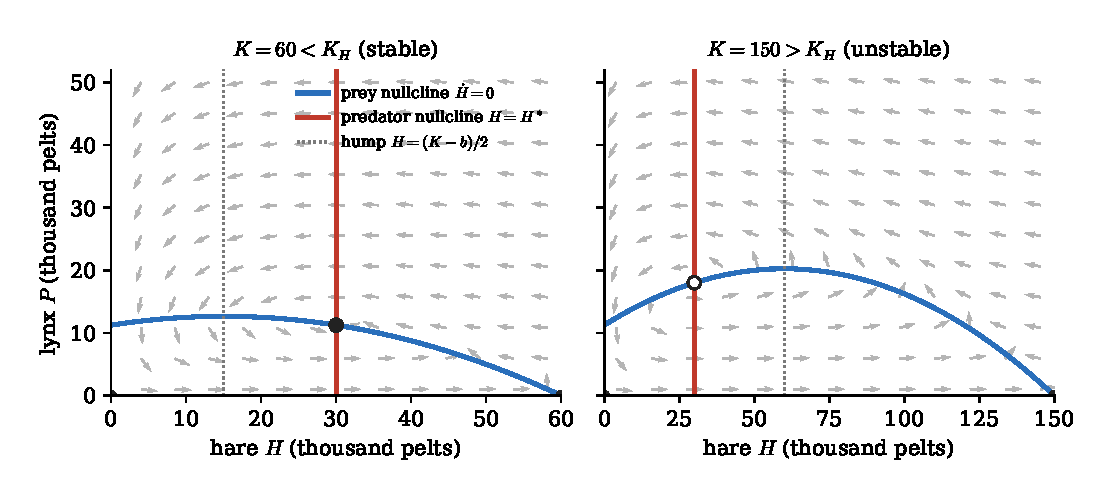
\includegraphics[width=\linewidth]{joel_nullclines}
\caption{Nullclines and direction field for the illustrative parameters
($r=1.5,\ a=4,\ b=30,\ e=0.4,\ m=0.8$; $H^*=30$, $K_H=90$).
Left: $K=60$; the predator nullcline meets the parabola right of its hump and $E^*$ (filled)
is a stable focus. Right: $K=150$; the intersection is left of the hump and $E^*$ (open) is
unstable. Small dots mark $E_0$ and $E_1$.}
\label{fig:nullclines}
\end{figure}

% ---------------------------------------------------------------------
\subsection{Hopf bifurcation with $K$ as the parameter}\label{sec:joel-hopf}

We fix $r,a,b,e,m$ with $ea>m$ and vary $K$ over $(H^*,\infty)$. Note $H^*$ is independent of
$K$, while $P^*$ increases with $K$.

\begin{theorem}[Hopf bifurcation]\label{thm:hopf}
At $K=K_H=b+2H^*$ the coexistence equilibrium undergoes a Hopf bifurcation:
\begin{enumerate}
\item[(i)] $\tau(E^*)=0$ and $\Delta(E^*)=\dfrac{rmb\,(K_H-H^*)}{K_H(b+H^*)}=\dfrac{rmb}{K_H}>0$,
so $J(E^*)$ has eigenvalues $\pm i\omega_0$ with
\[
\omega_0=\sqrt{\frac{rmb}{b+2H^*}},\qquad T_0=\frac{2\pi}{\omega_0};
\]
\item[(ii)] (transversality) the real part of the eigenvalues, $\tau/2$, crosses zero with
nonzero speed:
\[
\frac{d}{dK}\Bigl(\frac{\tau}{2}\Bigr)\Big|_{K=K_H}=\frac{rH^*}{2(b+H^*)(b+2H^*)}>0 .
\]
\end{enumerate}
\end{theorem}

\begin{proof}
(i) Substitute $K=K_H$ into~\eqref{eq:trace} and~\eqref{eq:det}; $K_H-H^*=b+H^*$ simplifies $\Delta$.
(ii) Differentiate~\eqref{eq:trace} in $K$: $\frac{d}{dK}\frac{K-K_H}{K}=\frac{K_H}{K^2}$, which equals
$1/K_H$ at $K=K_H$. All symbolic steps were checked with SymPy (\texttt{scripts/joel\_symbolic\_derivation.py}) and the closed forms are tested against the shared model code (\texttt{tests/test\_stability.py}).
\end{proof}

Conditions (i)--(ii) establish that a pair of complex eigenvalues crosses the imaginary axis.
To conclude that a small periodic orbit is born, and on which side, the Hopf theorem also needs
the first Lyapunov coefficient $\ell_1$ to be nonzero~\cite{kuznetsov2004}: $\ell_1<0$ gives a
\emph{supercritical} bifurcation (a stable cycle for $K>K_H$) and $\ell_1>0$ a subcritical one.

\paragraph{What is analytic and what is numerical.} We separate four statements.
\begin{enumerate}
\item \textbf{Analytic (derived here):} the threshold $K_H$, conditions (i)--(ii), and the
exchange of stability at $E^*$.
\item \textbf{Analytic (derived here): existence of a periodic orbit for $K>K_H$.}
Take any initial condition in the open quadrant. By Lemma~\ref{lem:bounded} its $\omega$-limit
set $\Omega$ is nonempty and compact. $\Omega$ cannot contain $E^*$, which is a repeller.
$\Omega$ cannot be $\{E_1\}$, because the stable manifold of the saddle $E_1$ is the $H$-axis.
If $\Omega$ contained $E_1$ together with other points, it would contain a point of $E_1$'s
stable manifold on the $H$-axis and hence the whole axis orbit through it, which tends backward
to $E_0$; repeating the argument at $E_0$ would put a point of the $P$-axis in $\Omega$, whose
backward orbit is unbounded, contradicting compactness. So $\Omega$ contains no equilibria, and
the Poincar\'e--Bendixson theorem~\cite{strogatz2015} makes $\Omega$ a periodic orbit.
\item \textbf{Cited theorems:} Cheng~\cite{cheng1981} proved the limit cycle is \emph{unique} for
$K>K_H$; since every interior orbit other than $E^*$ tends to a periodic orbit, that unique cycle
attracts them all and is orbitally stable. Hsu~\cite{hsu1978} proved that a locally stable $E^*$
is \emph{globally} stable in the open quadrant whenever the prey nullcline is concave, which our
parabola~\eqref{eq:prey-null} is, so $E^*$ attracts every interior orbit for $H^*<K<K_H$.
We use these results without reproducing their proofs.
\item \textbf{Numerical (for our parameter set only):} evaluating Kuznetsov's formula for
$\ell_1$ at $K=K_H$ gives $\ell_1\approx-4.0\times10^{-4}<0$ (and $-1.3\times10^{-3}$ for a second
set $r=0.7,\ m=0.5,\ b=20$), so the bifurcation is supercritical, consistent with the cited
uniqueness result. Simulations confirm the supercritical signature: the post-transient cycle
half-amplitude in $H$ scales as $(K-K_H)^{1/2}$ (fitted log--log slope $0.507$ for
$K-K_H\in[0.5,8]$), and the period tends to $T_0$.
\end{enumerate}

\noindent None of this says that the \emph{real} hare--lynx data sit on a limit cycle. That
depends on whether fitted parameters satisfy $K>K_H$, and with about two oscillations in
1900--1920 a slowly damped oscillation ($K$ slightly below $K_H$) can fit the same data.
That question belongs to the fitting sections and must be answered there with uncertainty.

\begin{figure}[ht]
\centering
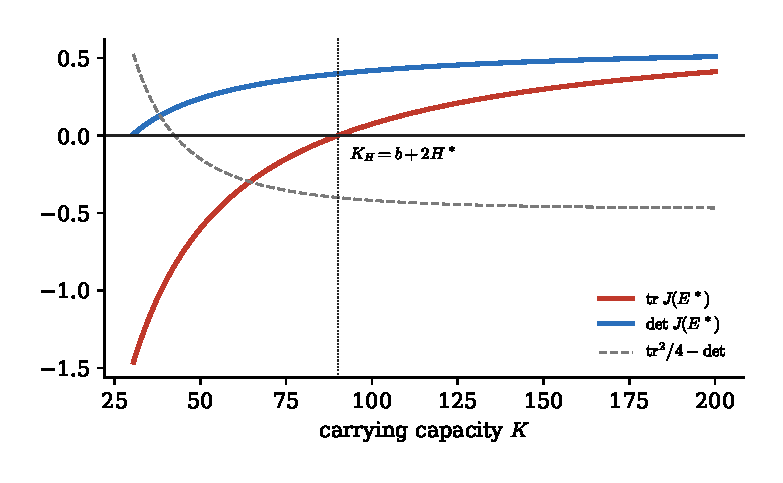
\includegraphics[width=0.7\linewidth]{joel_trace_det}
\caption{Trace and determinant of $J(E^*)$ as functions of $K$ (illustrative parameters).
The determinant stays positive for all feasible $K>H^*=30$, while the trace changes sign at
$K_H=90$. The dashed curve is negative (focus) for $K>42.5$.}
\label{fig:trace-det}
\end{figure}

% ---------------------------------------------------------------------
\subsection{The paradox of enrichment}

Increasing $K$ (enriching the hares' environment) leaves $H^*$ unchanged and only raises $P^*$:
every extra unit of carrying capacity is passed to the predator. Graphically, the prey parabola's
hump $(K-b)/2$ moves right while the predator nullcline stays at $H^*$, so for large enough $K$
the intersection falls left of the hump and the equilibrium destabilises. Past $K_H$ the system
settles on a limit cycle whose amplitude grows with $K$. For our illustrative parameters, at
$K=150$ the hare minimum on the cycle is about $1.1$ thousand, compared with $H^*=30$. In a
finite, stochastic population such deep troughs bring a real risk of extinction. Enrichment
thus \emph{destabilises} the system, the paradox named by Rosenzweig~\cite{rosenzweig1971}.

The mechanism is the saturating Holling type II response. At low $H$ each lynx's consumption
rises almost linearly with prey, which damps fluctuations; near and above $b$ it saturates, so
per-capita predation risk $aP/(b+H)$ \emph{falls} as hares increase. That positive feedback on
prey growth is exactly the term making $J_{11}>0$ left of the hump.

\paragraph{Link to Lotka--Volterra.} In the classical model ($K=\infty$, linear response) the
analogous Jacobian at coexistence has $\tau\equiv0$ for every parameter value, so it sits
permanently on the Hopf boundary. That is why its neutral cycles are structurally unstable: any
small change in the model's form moves it to one side or the other.
Rosenzweig--MacArthur makes the side explicit through the sign of $K-K_H$.

% ---------------------------------------------------------------------
\subsection{Illustrative regimes and numerical validation targets}\label{sec:joel-regimes}

These parameters are \emph{illustrative, not fitted}: $H$ and $P$ in thousands of pelts, $t$ in
years, with $r=1.5,\ a=4,\ b=30,\ e=0.4,\ m=0.8$. Then $ea=1.6=2m$, so $H^*=b=30$, $K_H=90$,
$\omega_0=\sqrt{0.4}\approx0.632$ and $T_0\approx9.94$ years, close to the observed decadal
cycle. Table~\ref{tab:joel-regimes} gives the expected behaviour on each side of the threshold;
the simulation section reproduces these with RK45 (\texttt{rtol}$=10^{-10}$,
\texttt{atol}$=10^{-12}$, 3000-year burn-in, start $(20,5)$).

\begin{table}[ht]
\centering
\small
\caption{Regimes in $K$ (other parameters fixed). Eigenvalues are of $J(E^*)$, except in A where
they are of $J(E_1)$.}
\label{tab:joel-regimes}
\setlength{\tabcolsep}{4pt}
\begin{tabular}{@{}cr l l l@{}}
\toprule
 & $K$ & Linear prediction & Eigenvalues & Long-run behaviour (simulated)\\
\midrule
A & 25  & $E^*$ infeasible ($K<H^*$) & $-1.5,\ -0.073$ & lynx die out; $\to(25,0)$\\
B & 60  & $E^*$ stable focus & $-0.188\pm0.515i$ & $\to(30,\,11.25)$, e-fold $\approx5$ yr\\
C & 85  & just below $K_H$ & $-0.022\pm0.623i$ & $\to(30,\,14.56)$, e-fold $\approx45$ yr\\
D & 90  & Hopf point & $\pm0.632i$ & very slow (algebraic) decay\\
E & 95  & just above $K_H$ & $+0.020\pm0.640i$ & cycle: $H\in[15.8,50.9]$, $P\in[9.8,20.8]$, $T=10.25$\\
F & 150 & well above $K_H$ & $+0.150\pm0.676i$ & cycle: $H\in[1.1,134.3]$, $P\in[1.7,41.2]$, $T=13.91$\\
\bottomrule
\end{tabular}
\end{table}

\noindent Two cautions for the numerics. At D the equilibrium is a weak focus ($\ell_1<0$), so
oscillations decay only like $t^{-1/2}$; after 3000 years the residual amplitude in $H$ is still
about $1.5$, which is expected and is not a sign of a cycle. The cycle at E is already large
because the amplitude coefficient is large ($A_H\approx7.8\sqrt{K-K_H}$), so ``small
amplitude'' only holds within about one unit of $K_H$.

\begin{figure}[ht]
\centering
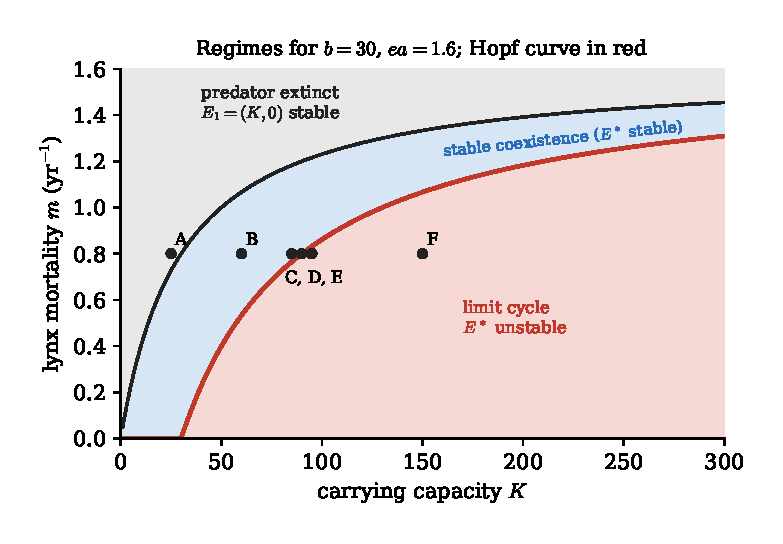
\includegraphics[width=0.7\linewidth]{joel_regions}
\caption{Analytic regimes in the $(K,m)$ plane for $b=30$, $ea=1.6$. Black curve:
$m=eaK/(b+K)$ (predator persistence boundary). Red curve: $m=ea(K-b)/(K+b)$ (Hopf curve).
Dots mark regimes A--F of Table~\ref{tab:joel-regimes}.}
\label{fig:regions}
\end{figure}

% ---------------------------------------------------------------------
\subsection{Sensitivity of the threshold}

Because $K_H=b(ea+m)/(ea-m)$ is explicit, sensitivity can be read off exactly. The elasticities
(percentage change in $K_H$ per percentage change in a parameter) are
\[
\frac{\partial\ln K_H}{\partial\ln b}=1,\qquad
\frac{\partial\ln K_H}{\partial\ln m}=-\frac{\partial\ln K_H}{\partial\ln a}
=-\frac{\partial\ln K_H}{\partial\ln e}=\frac{2\,ea\,m}{(ea)^2-m^2},\qquad
\frac{\partial\ln K_H}{\partial\ln r}=0.
\]
At the illustrative values ($ea=2m$) the middle elasticity is $4/3$: a 10\% rise in lynx
mortality raises the threshold by about 13\%, and so stabilises the system. The elasticity blows
up as $m\to ea$, where the predator is barely viable and $K_H\to\infty$. Weak predators stabilise.

Equivalently, for fixed $K$ the regimes are bands in $m$ (Figure~\ref{fig:regions}):
\[
\underbrace{m<\frac{ea(K-b)}{K+b}}_{\text{limit cycle}}
\qquad
\underbrace{\frac{ea(K-b)}{K+b}<m<\frac{eaK}{K+b}}_{\text{stable coexistence}}
\qquad
\underbrace{m>\frac{eaK}{K+b}}_{\text{lynx extinct}}
\]
A useful single number for any fitted parameter set is the \emph{stability margin}
$\sigma=K/K_H$: $\sigma<1$ means damped oscillations, $\sigma>1$ a limit cycle. Reporting
$\sigma$ (with its spread over fits) is the cleanest way to say whether the data support
sustained cycling.

Two structural facts matter for inference. First, $a$ and $e$ enter $H^*$, $K_H$ and the
stability conditions only through the product $ea$. Second, if lynx are measured only up to an
unknown multiplicative factor $c$ (as pelt counts are), the map $(P,a,e)\mapsto(cP,\,a/c,\,ec)$
leaves~\eqref{eq:rm} unchanged (checked symbolically), so $a$ and $e$ are \emph{not separately
identifiable} from index data. Fitting should fix one of them, or fit $ea$ and a scale, rather
than report both as biological rates.

% ---------------------------------------------------------------------
\subsection{Dimensionless form of the results}

With the scaling $x=H/K$, $y=aP/(rK)$, $s=rt$ (to be reconciled with the frozen scaling in the
model section), \eqref{eq:rm} becomes
\[
x'=x(1-x)-\frac{xy}{\beta+x},\qquad y'=y\Bigl(\frac{\alpha x}{\beta+x}-\delta\Bigr),
\qquad \beta=\frac{b}{K},\ \alpha=\frac{ea}{r},\ \delta=\frac{m}{r}.
\]
Then $x^*=\beta\delta/(\alpha-\delta)$, coexistence requires $\alpha>\delta$ and $x^*<1$, and the
Hopf condition $K=K_H$ reads $\beta(\alpha+\delta)/(\alpha-\delta)=1$, i.e.\ $\beta+2x^*=1$.
Only three combinations of the six parameters control the qualitative dynamics.

% ---------------------------------------------------------------------
\begin{table}[ht]
\centering
\small
\caption{Status of each stability claim in this section.}
\label{tab:joel-evidence}
\begin{tabular}{@{}p{0.52\linewidth}p{0.42\linewidth}@{}}
\toprule
Claim & Evidence \\
\midrule
Equilibria, feasibility, local stability of $E_0,E_1,E^*$ & Derived here; SymPy-checked\\
Hopf threshold $K_H=b+2H^*$, $\Delta>0$, transversality & Derived here; SymPy-checked\\
A periodic orbit exists for every $K>K_H$ & Derived here (Poincar\'e--Bendixson)\\
Cycle is unique and attracting for $K>K_H$ & Cited theorem~\cite{cheng1981}\\
$E^*$ globally stable for $H^*<K<K_H$ & Cited theorem~\cite{hsu1978}\\
Supercritical Hopf ($\ell_1<0$) & Numerical evaluation of analytic formula, two parameter sets\\
$\sqrt{K-K_H}$ amplitude law; periods, amplitudes, lags & Numerical (RK45), illustrative parameters\\
Real hare--lynx data lie on a limit cycle & \emph{Not established here}; requires $\sigma>1$ at fitted values with uncertainty\\
\bottomrule
\end{tabular}
\end{table}
   (standalone build: joel_main.tex)
%  Needs: amsmath, amssymb, amsthm (theorem, proposition, lemma, remark
%         environments), booktabs, graphicx (PDF companions are used under pdflatex)
%  Figures: graphs/joel_{nullclines,trace_det,regions}.{eps,pdf}
%  Regenerate: python scripts/joel_stability_analysis.py
%  Bibliography keys: in report/references.bib
% =====================================================================

\section{Equilibria, Stability and Hopf Bifurcation}\label{sec:joel}

Throughout this section we analyse the dimensional Rosenzweig--MacArthur model
\begin{equation}\label{eq:rm}
\frac{dH}{dt}= f(H,P) = rH\Bigl(1-\frac{H}{K}\Bigr)-\frac{aHP}{b+H},
\qquad
\frac{dP}{dt}= g(H,P) = \frac{eaHP}{b+H}-mP,
\end{equation}
with all six parameters $r,K,a,b,e,m$ strictly positive, as defined in the model section.
Every stability statement below is tied either to a derivation given here, to a
cited theorem, or to a numerical check; Table~\ref{tab:joel-evidence} at the end of the
section records which is which.

% ---------------------------------------------------------------------
\subsection{Well-posedness: invariance and boundedness}

\begin{lemma}\label{lem:bounded}
The closed quadrant $\{H\ge 0,\,P\ge 0\}$, both coordinate axes, and the open quadrant are
invariant under~\eqref{eq:rm}. Every solution starting in the quadrant is bounded, with
\[
\limsup_{t\to\infty} H(t)\le K,
\qquad
\limsup_{t\to\infty}\bigl(eH(t)+P(t)\bigr)\le \frac{eK(r+m)^2}{4rm}.
\]
\end{lemma}

\begin{proof}
Both right-hand sides factor as $H\cdot(\cdot)$ and $P\cdot(\cdot)$, so $H=0$ and $P=0$ are
invariant lines and, by uniqueness of solutions, no orbit can cross them. Since
$\dot H\le rH(1-H/K)$, comparison with the logistic equation gives $\limsup H\le K$.
For $W=eH+P$ the predation terms cancel:
$\dot W = erH(1-H/K)-mP = eH\bigl(r(1-H/K)+m\bigr)-mW$.
The quadratic $H\bigl(r(1-H/K)+m\bigr)$ is maximised at $H=K(r+m)/(2r)$ with value
$K(r+m)^2/(4r)$, so $\dot W\le eK(r+m)^2/(4r)-mW$ and the bound follows.
\end{proof}

Boundedness is what later allows the Poincar\'e--Bendixson theorem to be used.

% ---------------------------------------------------------------------
\subsection{Equilibria and biological feasibility}

Setting $f=g=0$:
\begin{itemize}
\item $P=0$ in $g=0$ leaves $rH(1-H/K)=0$, giving the \emph{origin} $E_0=(0,0)$ and the
\emph{prey-only} equilibrium $E_1=(K,0)$.
\item $P\neq 0$ requires $eaH/(b+H)=m$, i.e.
\begin{equation}\label{eq:Hstar}
H^*=\frac{mb}{ea-m},
\end{equation}
and then $f=0$ with $H=H^*\neq0$ gives
\begin{equation}\label{eq:Pstar}
P^*=\frac{r}{a}\Bigl(1-\frac{H^*}{K}\Bigr)(b+H^*)
=\frac{ebr\bigl(K(ea-m)-bm\bigr)}{K(ea-m)^2}.
\end{equation}
This is the \emph{coexistence} equilibrium $E^*=(H^*,P^*)$.
\end{itemize}

\begin{proposition}[Feasibility]\label{prop:feasible}
$E_0$ and $E_1$ always lie in the closed quadrant. $E^*$ lies in the open quadrant if and only if
\[
ea>m \quad\text{and}\quad H^*<K
\qquad\Longleftrightarrow\qquad
m<\frac{eaK}{b+K}.
\]
\end{proposition}

\begin{proof}
$H^*>0$ iff $ea>m$. Given this, $P^*>0$ iff $1-H^*/K>0$. Rearranging $mb/(ea-m)<K$
gives $m(b+K)<eaK$.
\end{proof}

\noindent Biologically, $ea$ is the predator's maximal per-capita birth rate (attained when prey is
abundant), so $ea>m$ says lynx can outgrow their mortality at all; $H^*<K$ says the hare
level lynx need to break even is actually reachable by the prey on its own. Note that
$H^*$ does not depend on $r$ or $K$: the prey level at coexistence is set entirely by the
predator.

% ---------------------------------------------------------------------
\subsection{Jacobian}

Differentiating~\eqref{eq:rm},
\begin{equation}\label{eq:jac}
J(H,P)=\begin{pmatrix}
r\Bigl(1-\dfrac{2H}{K}\Bigr)-\dfrac{abP}{(b+H)^2} & -\dfrac{aH}{b+H}\\[2ex]
\dfrac{eabP}{(b+H)^2} & \dfrac{eaH}{b+H}-m
\end{pmatrix}.
\end{equation}
For a planar system, with $\tau=\operatorname{tr}J$ and $\Delta=\det J$, an equilibrium is a
saddle if $\Delta<0$; is asymptotically stable if $\Delta>0,\ \tau<0$; and is unstable if
$\Delta>0,\ \tau>0$. It is a focus when $\tau^2<4\Delta$ and a node when $\tau^2>4\Delta$.

% ---------------------------------------------------------------------
\subsection{Local stability of each equilibrium}

\paragraph{Origin.} $J(E_0)=\operatorname{diag}(r,-m)$, with eigenvalues $r>0$ and $-m<0$.
$E_0$ is \emph{always a saddle}: the $P$-axis is its stable manifold (lynx alone die out) and the
$H$-axis its unstable manifold (hares alone grow). Joint extinction is never an attractor.

\paragraph{Prey-only equilibrium.}
\[
J(E_1)=\begin{pmatrix}-r & -\dfrac{aK}{b+K}\\[1.5ex] 0 & \dfrac{eaK}{b+K}-m\end{pmatrix},
\qquad
\lambda_1=-r,\quad \lambda_2=\frac{eaK}{b+K}-m .
\]
$E_1$ is a stable node when $\lambda_2<0$, i.e.\ exactly when $E^*$ is \emph{not} feasible, and a
saddle when $\lambda_2>0$, i.e.\ exactly when $E^*$ is feasible. At $K=H^*$ the two equilibria
coincide and exchange stability (a transcritical bifurcation). $\lambda_2$ is the invasion rate
of a rare lynx population into a hare population at carrying capacity.

\paragraph{Coexistence equilibrium.}
At $E^*$ the predator equation gives $eaH^*/(b+H^*)=m$, so $J_{22}=0$. Using the prey nullcline,
$aP^*/(b+H^*)=r(1-H^*/K)$, to eliminate $P^*$ from $J_{11}$:
\[
J_{11}=r\Bigl(1-\frac{2H^*}{K}\Bigr)-\frac{b}{b+H^*}\,r\Bigl(1-\frac{H^*}{K}\Bigr)
=\frac{rH^*\,(K-b-2H^*)}{K\,(b+H^*)} .
\]
Hence
\begin{align}
\tau(E^*) &= \frac{rH^*}{K(b+H^*)}\,\bigl(K-K_H\bigr),
\qquad K_H := b+2H^* = \frac{b\,(ea+m)}{ea-m}, \label{eq:trace}\\
\Delta(E^*) &= -J_{12}J_{21} = \frac{aH^*}{b+H^*}\cdot\frac{eabP^*}{(b+H^*)^2}
= \frac{rmb\,(K-H^*)}{K(b+H^*)}. \label{eq:det}
\end{align}

\begin{theorem}[Local stability of $E^*$]\label{thm:local}
Suppose $E^*$ is feasible ($H^*<K$). Then $\Delta(E^*)>0$, so $E^*$ is never a saddle, and
\[
E^* \text{ is locally asymptotically stable if } K<K_H,
\qquad
E^* \text{ is unstable (a repeller) if } K>K_H .
\]
\end{theorem}

\begin{proof}
$\Delta>0$ follows from~\eqref{eq:det} since $K>H^*$. The sign of $\tau$ is the sign of
$K-K_H$ by~\eqref{eq:trace}. Apply the trace--determinant classification.
\end{proof}

\begin{remark}
The intrinsic hare growth rate $r$ appears in $\tau$ and $\Delta$ only as a positive prefactor.
It therefore sets how fast trajectories spiral, but has \emph{no effect} on whether $E^*$ is stable.
Near feasibility ($K$ just above $H^*$), $\Delta\to0$ while $\tau<0$, so $E^*$ is a stable node;
as $K$ increases it becomes a stable focus once $\tau^2<4\Delta$ (at $K\approx42.5$ for the
illustrative parameters of \S\ref{sec:joel-regimes}), so convergence is oscillatory well before
the Hopf point.
\end{remark}

\begin{table}[ht]
\centering
\caption{Equilibria of~\eqref{eq:rm} and their local stability.}
\label{tab:joel-equilibria}
\small
\begin{tabular}{@{}l l l p{0.33\linewidth}@{}}
\toprule
Equilibrium & Feasible when & Eigenvalues / invariants & Type \\
\midrule
$E_0=(0,0)$ & always & $r,\ -m$ & saddle \\[0.5ex]
$E_1=(K,0)$ & always & $-r,\ \tfrac{eaK}{b+K}-m$ & stable node if $K<H^*$ or $ea\le m$; saddle if $K>H^*$\\[0.5ex]
$E^*=(H^*,P^*)$ & $ea>m,\ H^*<K$ & $\tau\propto K-K_H,\ \Delta>0$ & stable if $K<K_H$; unstable if $K>K_H$\\
\bottomrule
\end{tabular}
\end{table}

% ---------------------------------------------------------------------
\subsection{Nullclines and the phase plane}

\paragraph{Prey nullclines ($\dot H=0$):} the $P$-axis $H=0$, and the parabola
\begin{equation}\label{eq:prey-null}
P=\phi(H):=\frac{r}{a}\Bigl(1-\frac{H}{K}\Bigr)(b+H),
\end{equation}
which is concave, vanishes at $H=-b$ and $H=K$, cuts the $P$-axis at $rb/a$, and peaks at
\[
H_{\text{peak}}=\frac{K-b}{2},\qquad \phi(H_{\text{peak}})=\frac{r(K+b)^2}{4aK}.
\]
$\dot H>0$ below the parabola and $\dot H<0$ above it (for $H>0$).

\paragraph{Predator nullclines ($\dot P=0$):} the $H$-axis $P=0$, and the vertical line
$H=H^*$. $\dot P>0$ to the right of $H=H^*$ (enough prey) and $\dot P<0$ to the left.

\paragraph{Flow.} The two interior nullclines divide the open quadrant into four regions.
Starting below the parabola to the right of $H^*$, both species increase; crossing the parabola
hares start to fall while lynx still rise; crossing $H=H^*$ both fall; crossing back below the
parabola hares recover while lynx are still falling. The flow therefore circulates
\emph{counter-clockwise} around $E^*$ in the $(H,P)$ plane, and lynx peaks lag hare peaks.
Near the Hopf point the lag is a quarter-period; it grows with $K$ (numerically, $2.5$ to $4.5$
years for regimes D--F below).

\paragraph{Graphical stability criterion.} Since $K_H=b+2H^*$ is equivalent to
$H^*=(K-b)/2=H_{\text{peak}}$, Theorem~\ref{thm:local} says:
\begin{center}
\emph{$E^*$ is stable if the predator nullcline cuts the prey parabola to the right of its hump,
and unstable if it cuts to the left.}
\end{center}
This is the original Rosenzweig--MacArthur graphical criterion~\cite{rosenzweig1963}. It also
gives the sign of $J_{11}$ directly: $J_{11}=a\,H^*\phi'(H^*)/(b+H^*)$, so a rising nullcline
(left of the hump) means local prey self-amplification ($J_{11}>0$). Figure~\ref{fig:nullclines} shows both cases.

\begin{figure}[ht]
\centering
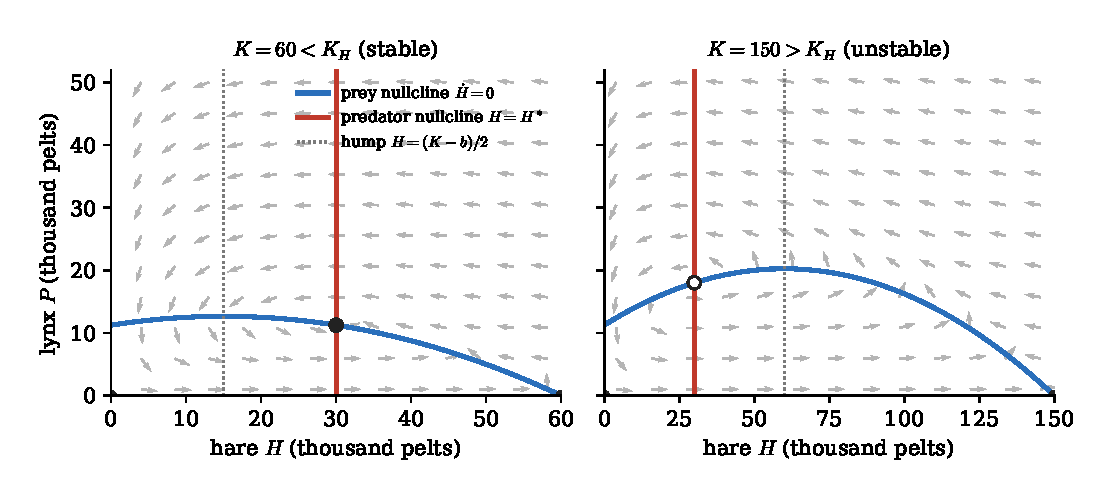
\includegraphics[width=\linewidth]{joel_nullclines}
\caption{Nullclines and direction field for the illustrative parameters
($r=1.5,\ a=4,\ b=30,\ e=0.4,\ m=0.8$; $H^*=30$, $K_H=90$).
Left: $K=60$; the predator nullcline meets the parabola right of its hump and $E^*$ (filled)
is a stable focus. Right: $K=150$; the intersection is left of the hump and $E^*$ (open) is
unstable. Small dots mark $E_0$ and $E_1$.}
\label{fig:nullclines}
\end{figure}

% ---------------------------------------------------------------------
\subsection{Hopf bifurcation with $K$ as the parameter}\label{sec:joel-hopf}

We fix $r,a,b,e,m$ with $ea>m$ and vary $K$ over $(H^*,\infty)$. Note $H^*$ is independent of
$K$, while $P^*$ increases with $K$.

\begin{theorem}[Hopf bifurcation]\label{thm:hopf}
At $K=K_H=b+2H^*$ the coexistence equilibrium undergoes a Hopf bifurcation:
\begin{enumerate}
\item[(i)] $\tau(E^*)=0$ and $\Delta(E^*)=\dfrac{rmb\,(K_H-H^*)}{K_H(b+H^*)}=\dfrac{rmb}{K_H}>0$,
so $J(E^*)$ has eigenvalues $\pm i\omega_0$ with
\[
\omega_0=\sqrt{\frac{rmb}{b+2H^*}},\qquad T_0=\frac{2\pi}{\omega_0};
\]
\item[(ii)] (transversality) the real part of the eigenvalues, $\tau/2$, crosses zero with
nonzero speed:
\[
\frac{d}{dK}\Bigl(\frac{\tau}{2}\Bigr)\Big|_{K=K_H}=\frac{rH^*}{2(b+H^*)(b+2H^*)}>0 .
\]
\end{enumerate}
\end{theorem}

\begin{proof}
(i) Substitute $K=K_H$ into~\eqref{eq:trace} and~\eqref{eq:det}; $K_H-H^*=b+H^*$ simplifies $\Delta$.
(ii) Differentiate~\eqref{eq:trace} in $K$: $\frac{d}{dK}\frac{K-K_H}{K}=\frac{K_H}{K^2}$, which equals
$1/K_H$ at $K=K_H$. All symbolic steps were checked with SymPy (\texttt{scripts/joel\_symbolic\_derivation.py}) and the closed forms are tested against the shared model code (\texttt{tests/test\_stability.py}).
\end{proof}

Conditions (i)--(ii) establish that a pair of complex eigenvalues crosses the imaginary axis.
To conclude that a small periodic orbit is born, and on which side, the Hopf theorem also needs
the first Lyapunov coefficient $\ell_1$ to be nonzero~\cite{kuznetsov2004}: $\ell_1<0$ gives a
\emph{supercritical} bifurcation (a stable cycle for $K>K_H$) and $\ell_1>0$ a subcritical one.

\paragraph{What is analytic and what is numerical.} We separate four statements.
\begin{enumerate}
\item \textbf{Analytic (derived here):} the threshold $K_H$, conditions (i)--(ii), and the
exchange of stability at $E^*$.
\item \textbf{Analytic (derived here): existence of a periodic orbit for $K>K_H$.}
Take any initial condition in the open quadrant. By Lemma~\ref{lem:bounded} its $\omega$-limit
set $\Omega$ is nonempty and compact. $\Omega$ cannot contain $E^*$, which is a repeller.
$\Omega$ cannot be $\{E_1\}$, because the stable manifold of the saddle $E_1$ is the $H$-axis.
If $\Omega$ contained $E_1$ together with other points, it would contain a point of $E_1$'s
stable manifold on the $H$-axis and hence the whole axis orbit through it, which tends backward
to $E_0$; repeating the argument at $E_0$ would put a point of the $P$-axis in $\Omega$, whose
backward orbit is unbounded, contradicting compactness. So $\Omega$ contains no equilibria, and
the Poincar\'e--Bendixson theorem~\cite{strogatz2015} makes $\Omega$ a periodic orbit.
\item \textbf{Cited theorems:} Cheng~\cite{cheng1981} proved the limit cycle is \emph{unique} for
$K>K_H$; since every interior orbit other than $E^*$ tends to a periodic orbit, that unique cycle
attracts them all and is orbitally stable. Hsu~\cite{hsu1978} proved that a locally stable $E^*$
is \emph{globally} stable in the open quadrant whenever the prey nullcline is concave, which our
parabola~\eqref{eq:prey-null} is, so $E^*$ attracts every interior orbit for $H^*<K<K_H$.
We use these results without reproducing their proofs.
\item \textbf{Numerical (for our parameter set only):} evaluating Kuznetsov's formula for
$\ell_1$ at $K=K_H$ gives $\ell_1\approx-4.0\times10^{-4}<0$ (and $-1.3\times10^{-3}$ for a second
set $r=0.7,\ m=0.5,\ b=20$), so the bifurcation is supercritical, consistent with the cited
uniqueness result. Simulations confirm the supercritical signature: the post-transient cycle
half-amplitude in $H$ scales as $(K-K_H)^{1/2}$ (fitted log--log slope $0.507$ for
$K-K_H\in[0.5,8]$), and the period tends to $T_0$.
\end{enumerate}

\noindent None of this says that the \emph{real} hare--lynx data sit on a limit cycle. That
depends on whether fitted parameters satisfy $K>K_H$, and with about two oscillations in
1900--1920 a slowly damped oscillation ($K$ slightly below $K_H$) can fit the same data.
That question belongs to the fitting sections and must be answered there with uncertainty.

\begin{figure}[ht]
\centering
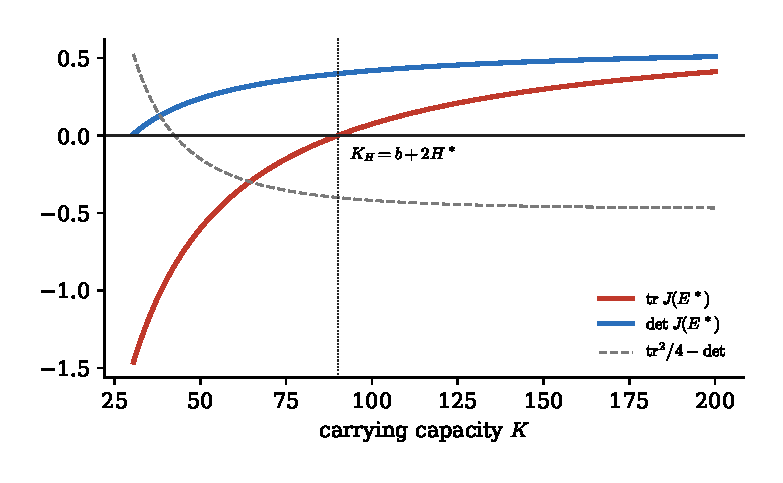
\includegraphics[width=0.7\linewidth]{joel_trace_det}
\caption{Trace and determinant of $J(E^*)$ as functions of $K$ (illustrative parameters).
The determinant stays positive for all feasible $K>H^*=30$, while the trace changes sign at
$K_H=90$. The dashed curve is negative (focus) for $K>42.5$.}
\label{fig:trace-det}
\end{figure}

% ---------------------------------------------------------------------
\subsection{The paradox of enrichment}

Increasing $K$ (enriching the hares' environment) leaves $H^*$ unchanged and only raises $P^*$:
every extra unit of carrying capacity is passed to the predator. Graphically, the prey parabola's
hump $(K-b)/2$ moves right while the predator nullcline stays at $H^*$, so for large enough $K$
the intersection falls left of the hump and the equilibrium destabilises. Past $K_H$ the system
settles on a limit cycle whose amplitude grows with $K$. For our illustrative parameters, at
$K=150$ the hare minimum on the cycle is about $1.1$ thousand, compared with $H^*=30$. In a
finite, stochastic population such deep troughs bring a real risk of extinction. Enrichment
thus \emph{destabilises} the system, the paradox named by Rosenzweig~\cite{rosenzweig1971}.

The mechanism is the saturating Holling type II response. At low $H$ each lynx's consumption
rises almost linearly with prey, which damps fluctuations; near and above $b$ it saturates, so
per-capita predation risk $aP/(b+H)$ \emph{falls} as hares increase. That positive feedback on
prey growth is exactly the term making $J_{11}>0$ left of the hump.

\paragraph{Link to Lotka--Volterra.} In the classical model ($K=\infty$, linear response) the
analogous Jacobian at coexistence has $\tau\equiv0$ for every parameter value, so it sits
permanently on the Hopf boundary. That is why its neutral cycles are structurally unstable: any
small change in the model's form moves it to one side or the other.
Rosenzweig--MacArthur makes the side explicit through the sign of $K-K_H$.

% ---------------------------------------------------------------------
\subsection{Illustrative regimes and numerical validation targets}\label{sec:joel-regimes}

These parameters are \emph{illustrative, not fitted}: $H$ and $P$ in thousands of pelts, $t$ in
years, with $r=1.5,\ a=4,\ b=30,\ e=0.4,\ m=0.8$. Then $ea=1.6=2m$, so $H^*=b=30$, $K_H=90$,
$\omega_0=\sqrt{0.4}\approx0.632$ and $T_0\approx9.94$ years, close to the observed decadal
cycle. Table~\ref{tab:joel-regimes} gives the expected behaviour on each side of the threshold;
the simulation section reproduces these with RK45 (\texttt{rtol}$=10^{-10}$,
\texttt{atol}$=10^{-12}$, 3000-year burn-in, start $(20,5)$).

\begin{table}[ht]
\centering
\small
\caption{Regimes in $K$ (other parameters fixed). Eigenvalues are of $J(E^*)$, except in A where
they are of $J(E_1)$.}
\label{tab:joel-regimes}
\setlength{\tabcolsep}{4pt}
\begin{tabular}{@{}cr l l l@{}}
\toprule
 & $K$ & Linear prediction & Eigenvalues & Long-run behaviour (simulated)\\
\midrule
A & 25  & $E^*$ infeasible ($K<H^*$) & $-1.5,\ -0.073$ & lynx die out; $\to(25,0)$\\
B & 60  & $E^*$ stable focus & $-0.188\pm0.515i$ & $\to(30,\,11.25)$, e-fold $\approx5$ yr\\
C & 85  & just below $K_H$ & $-0.022\pm0.623i$ & $\to(30,\,14.56)$, e-fold $\approx45$ yr\\
D & 90  & Hopf point & $\pm0.632i$ & very slow (algebraic) decay\\
E & 95  & just above $K_H$ & $+0.020\pm0.640i$ & cycle: $H\in[15.8,50.9]$, $P\in[9.8,20.8]$, $T=10.25$\\
F & 150 & well above $K_H$ & $+0.150\pm0.676i$ & cycle: $H\in[1.1,134.3]$, $P\in[1.7,41.2]$, $T=13.91$\\
\bottomrule
\end{tabular}
\end{table}

\noindent Two cautions for the numerics. At D the equilibrium is a weak focus ($\ell_1<0$), so
oscillations decay only like $t^{-1/2}$; after 3000 years the residual amplitude in $H$ is still
about $1.5$, which is expected and is not a sign of a cycle. The cycle at E is already large
because the amplitude coefficient is large ($A_H\approx7.8\sqrt{K-K_H}$), so ``small
amplitude'' only holds within about one unit of $K_H$.

\begin{figure}[ht]
\centering
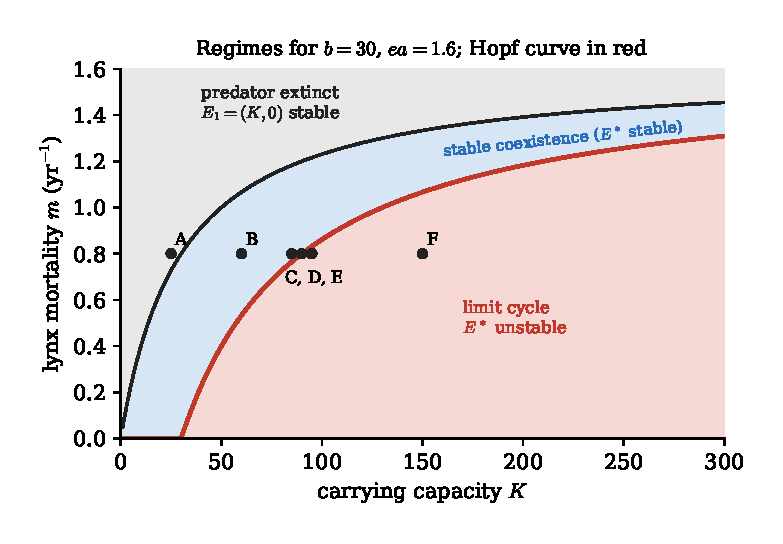
\includegraphics[width=0.7\linewidth]{joel_regions}
\caption{Analytic regimes in the $(K,m)$ plane for $b=30$, $ea=1.6$. Black curve:
$m=eaK/(b+K)$ (predator persistence boundary). Red curve: $m=ea(K-b)/(K+b)$ (Hopf curve).
Dots mark regimes A--F of Table~\ref{tab:joel-regimes}.}
\label{fig:regions}
\end{figure}

% ---------------------------------------------------------------------
\subsection{Sensitivity of the threshold}

Because $K_H=b(ea+m)/(ea-m)$ is explicit, sensitivity can be read off exactly. The elasticities
(percentage change in $K_H$ per percentage change in a parameter) are
\[
\frac{\partial\ln K_H}{\partial\ln b}=1,\qquad
\frac{\partial\ln K_H}{\partial\ln m}=-\frac{\partial\ln K_H}{\partial\ln a}
=-\frac{\partial\ln K_H}{\partial\ln e}=\frac{2\,ea\,m}{(ea)^2-m^2},\qquad
\frac{\partial\ln K_H}{\partial\ln r}=0.
\]
At the illustrative values ($ea=2m$) the middle elasticity is $4/3$: a 10\% rise in lynx
mortality raises the threshold by about 13\%, and so stabilises the system. The elasticity blows
up as $m\to ea$, where the predator is barely viable and $K_H\to\infty$. Weak predators stabilise.

Equivalently, for fixed $K$ the regimes are bands in $m$ (Figure~\ref{fig:regions}):
\[
\underbrace{m<\frac{ea(K-b)}{K+b}}_{\text{limit cycle}}
\qquad
\underbrace{\frac{ea(K-b)}{K+b}<m<\frac{eaK}{K+b}}_{\text{stable coexistence}}
\qquad
\underbrace{m>\frac{eaK}{K+b}}_{\text{lynx extinct}}
\]
A useful single number for any fitted parameter set is the \emph{stability margin}
$\sigma=K/K_H$: $\sigma<1$ means damped oscillations, $\sigma>1$ a limit cycle. Reporting
$\sigma$ (with its spread over fits) is the cleanest way to say whether the data support
sustained cycling.

Two structural facts matter for inference. First, $a$ and $e$ enter $H^*$, $K_H$ and the
stability conditions only through the product $ea$. Second, if lynx are measured only up to an
unknown multiplicative factor $c$ (as pelt counts are), the map $(P,a,e)\mapsto(cP,\,a/c,\,ec)$
leaves~\eqref{eq:rm} unchanged (checked symbolically), so $a$ and $e$ are \emph{not separately
identifiable} from index data. Fitting should fix one of them, or fit $ea$ and a scale, rather
than report both as biological rates.

% ---------------------------------------------------------------------
\subsection{Dimensionless form of the results}

With the scaling $x=H/K$, $y=aP/(rK)$, $s=rt$ (to be reconciled with the frozen scaling in the
model section), \eqref{eq:rm} becomes
\[
x'=x(1-x)-\frac{xy}{\beta+x},\qquad y'=y\Bigl(\frac{\alpha x}{\beta+x}-\delta\Bigr),
\qquad \beta=\frac{b}{K},\ \alpha=\frac{ea}{r},\ \delta=\frac{m}{r}.
\]
Then $x^*=\beta\delta/(\alpha-\delta)$, coexistence requires $\alpha>\delta$ and $x^*<1$, and the
Hopf condition $K=K_H$ reads $\beta(\alpha+\delta)/(\alpha-\delta)=1$, i.e.\ $\beta+2x^*=1$.
Only three combinations of the six parameters control the qualitative dynamics.

% ---------------------------------------------------------------------
\begin{table}[ht]
\centering
\small
\caption{Status of each stability claim in this section.}
\label{tab:joel-evidence}
\begin{tabular}{@{}p{0.52\linewidth}p{0.42\linewidth}@{}}
\toprule
Claim & Evidence \\
\midrule
Equilibria, feasibility, local stability of $E_0,E_1,E^*$ & Derived here; SymPy-checked\\
Hopf threshold $K_H=b+2H^*$, $\Delta>0$, transversality & Derived here; SymPy-checked\\
A periodic orbit exists for every $K>K_H$ & Derived here (Poincar\'e--Bendixson)\\
Cycle is unique and attracting for $K>K_H$ & Cited theorem~\cite{cheng1981}\\
$E^*$ globally stable for $H^*<K<K_H$ & Cited theorem~\cite{hsu1978}\\
Supercritical Hopf ($\ell_1<0$) & Numerical evaluation of analytic formula, two parameter sets\\
$\sqrt{K-K_H}$ amplitude law; periods, amplitudes, lags & Numerical (RK45), illustrative parameters\\
Real hare--lynx data lie on a limit cycle & \emph{Not established here}; requires $\sigma>1$ at fitted values with uncertainty\\
\bottomrule
\end{tabular}
\end{table}
   (standalone build: joel_main.tex)
%  Needs: amsmath, amssymb, amsthm (theorem, proposition, lemma, remark
%         environments), booktabs, graphicx (PDF companions are used under pdflatex)
%  Figures: graphs/joel_{nullclines,trace_det,regions}.{eps,pdf}
%  Regenerate: python scripts/joel_stability_analysis.py
%  Bibliography keys: in report/references.bib
% =====================================================================

\section{Equilibria, Stability and Hopf Bifurcation}\label{sec:joel}

Throughout this section we analyse the dimensional Rosenzweig--MacArthur model
\begin{equation}\label{eq:rm}
\frac{dH}{dt}= f(H,P) = rH\Bigl(1-\frac{H}{K}\Bigr)-\frac{aHP}{b+H},
\qquad
\frac{dP}{dt}= g(H,P) = \frac{eaHP}{b+H}-mP,
\end{equation}
with all six parameters $r,K,a,b,e,m$ strictly positive, as defined in the model section.
Every stability statement below is tied either to a derivation given here, to a
cited theorem, or to a numerical check; Table~\ref{tab:joel-evidence} at the end of the
section records which is which.

% ---------------------------------------------------------------------
\subsection{Well-posedness: invariance and boundedness}

\begin{lemma}\label{lem:bounded}
The closed quadrant $\{H\ge 0,\,P\ge 0\}$, both coordinate axes, and the open quadrant are
invariant under~\eqref{eq:rm}. Every solution starting in the quadrant is bounded, with
\[
\limsup_{t\to\infty} H(t)\le K,
\qquad
\limsup_{t\to\infty}\bigl(eH(t)+P(t)\bigr)\le \frac{eK(r+m)^2}{4rm}.
\]
\end{lemma}

\begin{proof}
Both right-hand sides factor as $H\cdot(\cdot)$ and $P\cdot(\cdot)$, so $H=0$ and $P=0$ are
invariant lines and, by uniqueness of solutions, no orbit can cross them. Since
$\dot H\le rH(1-H/K)$, comparison with the logistic equation gives $\limsup H\le K$.
For $W=eH+P$ the predation terms cancel:
$\dot W = erH(1-H/K)-mP = eH\bigl(r(1-H/K)+m\bigr)-mW$.
The quadratic $H\bigl(r(1-H/K)+m\bigr)$ is maximised at $H=K(r+m)/(2r)$ with value
$K(r+m)^2/(4r)$, so $\dot W\le eK(r+m)^2/(4r)-mW$ and the bound follows.
\end{proof}

Boundedness is what later allows the Poincar\'e--Bendixson theorem to be used.

% ---------------------------------------------------------------------
\subsection{Equilibria and biological feasibility}

Setting $f=g=0$:
\begin{itemize}
\item $P=0$ in $g=0$ leaves $rH(1-H/K)=0$, giving the \emph{origin} $E_0=(0,0)$ and the
\emph{prey-only} equilibrium $E_1=(K,0)$.
\item $P\neq 0$ requires $eaH/(b+H)=m$, i.e.
\begin{equation}\label{eq:Hstar}
H^*=\frac{mb}{ea-m},
\end{equation}
and then $f=0$ with $H=H^*\neq0$ gives
\begin{equation}\label{eq:Pstar}
P^*=\frac{r}{a}\Bigl(1-\frac{H^*}{K}\Bigr)(b+H^*)
=\frac{ebr\bigl(K(ea-m)-bm\bigr)}{K(ea-m)^2}.
\end{equation}
This is the \emph{coexistence} equilibrium $E^*=(H^*,P^*)$.
\end{itemize}

\begin{proposition}[Feasibility]\label{prop:feasible}
$E_0$ and $E_1$ always lie in the closed quadrant. $E^*$ lies in the open quadrant if and only if
\[
ea>m \quad\text{and}\quad H^*<K
\qquad\Longleftrightarrow\qquad
m<\frac{eaK}{b+K}.
\]
\end{proposition}

\begin{proof}
$H^*>0$ iff $ea>m$. Given this, $P^*>0$ iff $1-H^*/K>0$. Rearranging $mb/(ea-m)<K$
gives $m(b+K)<eaK$.
\end{proof}

\noindent Biologically, $ea$ is the predator's maximal per-capita birth rate (attained when prey is
abundant), so $ea>m$ says lynx can outgrow their mortality at all; $H^*<K$ says the hare
level lynx need to break even is actually reachable by the prey on its own. Note that
$H^*$ does not depend on $r$ or $K$: the prey level at coexistence is set entirely by the
predator.

% ---------------------------------------------------------------------
\subsection{Jacobian}

Differentiating~\eqref{eq:rm},
\begin{equation}\label{eq:jac}
J(H,P)=\begin{pmatrix}
r\Bigl(1-\dfrac{2H}{K}\Bigr)-\dfrac{abP}{(b+H)^2} & -\dfrac{aH}{b+H}\\[2ex]
\dfrac{eabP}{(b+H)^2} & \dfrac{eaH}{b+H}-m
\end{pmatrix}.
\end{equation}
For a planar system, with $\tau=\operatorname{tr}J$ and $\Delta=\det J$, an equilibrium is a
saddle if $\Delta<0$; is asymptotically stable if $\Delta>0,\ \tau<0$; and is unstable if
$\Delta>0,\ \tau>0$. It is a focus when $\tau^2<4\Delta$ and a node when $\tau^2>4\Delta$.

% ---------------------------------------------------------------------
\subsection{Local stability of each equilibrium}

\paragraph{Origin.} $J(E_0)=\operatorname{diag}(r,-m)$, with eigenvalues $r>0$ and $-m<0$.
$E_0$ is \emph{always a saddle}: the $P$-axis is its stable manifold (lynx alone die out) and the
$H$-axis its unstable manifold (hares alone grow). Joint extinction is never an attractor.

\paragraph{Prey-only equilibrium.}
\[
J(E_1)=\begin{pmatrix}-r & -\dfrac{aK}{b+K}\\[1.5ex] 0 & \dfrac{eaK}{b+K}-m\end{pmatrix},
\qquad
\lambda_1=-r,\quad \lambda_2=\frac{eaK}{b+K}-m .
\]
$E_1$ is a stable node when $\lambda_2<0$, i.e.\ exactly when $E^*$ is \emph{not} feasible, and a
saddle when $\lambda_2>0$, i.e.\ exactly when $E^*$ is feasible. At $K=H^*$ the two equilibria
coincide and exchange stability (a transcritical bifurcation). $\lambda_2$ is the invasion rate
of a rare lynx population into a hare population at carrying capacity.

\paragraph{Coexistence equilibrium.}
At $E^*$ the predator equation gives $eaH^*/(b+H^*)=m$, so $J_{22}=0$. Using the prey nullcline,
$aP^*/(b+H^*)=r(1-H^*/K)$, to eliminate $P^*$ from $J_{11}$:
\[
J_{11}=r\Bigl(1-\frac{2H^*}{K}\Bigr)-\frac{b}{b+H^*}\,r\Bigl(1-\frac{H^*}{K}\Bigr)
=\frac{rH^*\,(K-b-2H^*)}{K\,(b+H^*)} .
\]
Hence
\begin{align}
\tau(E^*) &= \frac{rH^*}{K(b+H^*)}\,\bigl(K-K_H\bigr),
\qquad K_H := b+2H^* = \frac{b\,(ea+m)}{ea-m}, \label{eq:trace}\\
\Delta(E^*) &= -J_{12}J_{21} = \frac{aH^*}{b+H^*}\cdot\frac{eabP^*}{(b+H^*)^2}
= \frac{rmb\,(K-H^*)}{K(b+H^*)}. \label{eq:det}
\end{align}

\begin{theorem}[Local stability of $E^*$]\label{thm:local}
Suppose $E^*$ is feasible ($H^*<K$). Then $\Delta(E^*)>0$, so $E^*$ is never a saddle, and
\[
E^* \text{ is locally asymptotically stable if } K<K_H,
\qquad
E^* \text{ is unstable (a repeller) if } K>K_H .
\]
\end{theorem}

\begin{proof}
$\Delta>0$ follows from~\eqref{eq:det} since $K>H^*$. The sign of $\tau$ is the sign of
$K-K_H$ by~\eqref{eq:trace}. Apply the trace--determinant classification.
\end{proof}

\begin{remark}
The intrinsic hare growth rate $r$ appears in $\tau$ and $\Delta$ only as a positive prefactor.
It therefore sets how fast trajectories spiral, but has \emph{no effect} on whether $E^*$ is stable.
Near feasibility ($K$ just above $H^*$), $\Delta\to0$ while $\tau<0$, so $E^*$ is a stable node;
as $K$ increases it becomes a stable focus once $\tau^2<4\Delta$ (at $K\approx42.5$ for the
illustrative parameters of \S\ref{sec:joel-regimes}), so convergence is oscillatory well before
the Hopf point.
\end{remark}

\begin{table}[ht]
\centering
\caption{Equilibria of~\eqref{eq:rm} and their local stability.}
\label{tab:joel-equilibria}
\small
\begin{tabular}{@{}l l l p{0.33\linewidth}@{}}
\toprule
Equilibrium & Feasible when & Eigenvalues / invariants & Type \\
\midrule
$E_0=(0,0)$ & always & $r,\ -m$ & saddle \\[0.5ex]
$E_1=(K,0)$ & always & $-r,\ \tfrac{eaK}{b+K}-m$ & stable node if $K<H^*$ or $ea\le m$; saddle if $K>H^*$\\[0.5ex]
$E^*=(H^*,P^*)$ & $ea>m,\ H^*<K$ & $\tau\propto K-K_H,\ \Delta>0$ & stable if $K<K_H$; unstable if $K>K_H$\\
\bottomrule
\end{tabular}
\end{table}

% ---------------------------------------------------------------------
\subsection{Nullclines and the phase plane}

\paragraph{Prey nullclines ($\dot H=0$):} the $P$-axis $H=0$, and the parabola
\begin{equation}\label{eq:prey-null}
P=\phi(H):=\frac{r}{a}\Bigl(1-\frac{H}{K}\Bigr)(b+H),
\end{equation}
which is concave, vanishes at $H=-b$ and $H=K$, cuts the $P$-axis at $rb/a$, and peaks at
\[
H_{\text{peak}}=\frac{K-b}{2},\qquad \phi(H_{\text{peak}})=\frac{r(K+b)^2}{4aK}.
\]
$\dot H>0$ below the parabola and $\dot H<0$ above it (for $H>0$).

\paragraph{Predator nullclines ($\dot P=0$):} the $H$-axis $P=0$, and the vertical line
$H=H^*$. $\dot P>0$ to the right of $H=H^*$ (enough prey) and $\dot P<0$ to the left.

\paragraph{Flow.} The two interior nullclines divide the open quadrant into four regions.
Starting below the parabola to the right of $H^*$, both species increase; crossing the parabola
hares start to fall while lynx still rise; crossing $H=H^*$ both fall; crossing back below the
parabola hares recover while lynx are still falling. The flow therefore circulates
\emph{counter-clockwise} around $E^*$ in the $(H,P)$ plane, and lynx peaks lag hare peaks.
Near the Hopf point the lag is a quarter-period; it grows with $K$ (numerically, $2.5$ to $4.5$
years for regimes D--F below).

\paragraph{Graphical stability criterion.} Since $K_H=b+2H^*$ is equivalent to
$H^*=(K-b)/2=H_{\text{peak}}$, Theorem~\ref{thm:local} says:
\begin{center}
\emph{$E^*$ is stable if the predator nullcline cuts the prey parabola to the right of its hump,
and unstable if it cuts to the left.}
\end{center}
This is the original Rosenzweig--MacArthur graphical criterion~\cite{rosenzweig1963}. It also
gives the sign of $J_{11}$ directly: $J_{11}=a\,H^*\phi'(H^*)/(b+H^*)$, so a rising nullcline
(left of the hump) means local prey self-amplification ($J_{11}>0$). Figure~\ref{fig:nullclines} shows both cases.

\begin{figure}[ht]
\centering
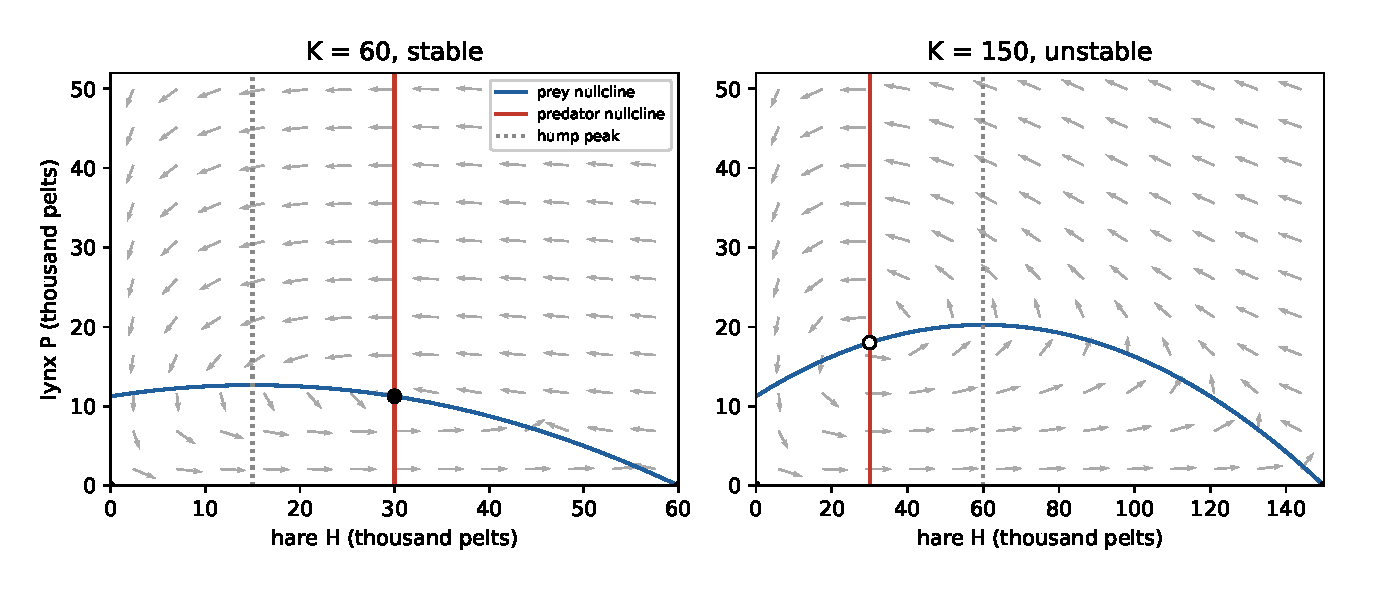
\includegraphics[width=\linewidth]{group_nullclines}
\caption{Nullclines and direction field for the illustrative parameters
($r=1.5,\ a=4,\ b=30,\ e=0.4,\ m=0.8$; $H^*=30$, $K_H=90$).
Left: $K=60$; the predator nullcline meets the parabola right of its hump and $E^*$ (filled)
is a stable focus. Right: $K=150$; the intersection is left of the hump and $E^*$ (open) is
unstable. Small dots mark $E_0$ and $E_1$.}
\label{fig:nullclines}
\end{figure}

% ---------------------------------------------------------------------
\subsection{Hopf bifurcation with $K$ as the parameter}\label{sec:joel-hopf}

We fix $r,a,b,e,m$ with $ea>m$ and vary $K$ over $(H^*,\infty)$. Note $H^*$ is independent of
$K$, while $P^*$ increases with $K$.

\begin{theorem}[Hopf bifurcation]\label{thm:hopf}
At $K=K_H=b+2H^*$ the coexistence equilibrium undergoes a Hopf bifurcation:
\begin{enumerate}
\item[(i)] $\tau(E^*)=0$ and $\Delta(E^*)=\dfrac{rmb\,(K_H-H^*)}{K_H(b+H^*)}=\dfrac{rmb}{K_H}>0$,
so $J(E^*)$ has eigenvalues $\pm i\omega_0$ with
\[
\omega_0=\sqrt{\frac{rmb}{b+2H^*}},\qquad T_0=\frac{2\pi}{\omega_0};
\]
\item[(ii)] (transversality) the real part of the eigenvalues, $\tau/2$, crosses zero with
nonzero speed:
\[
\frac{d}{dK}\Bigl(\frac{\tau}{2}\Bigr)\Big|_{K=K_H}=\frac{rH^*}{2(b+H^*)(b+2H^*)}>0 .
\]
\end{enumerate}
\end{theorem}

\begin{proof}
(i) Substitute $K=K_H$ into~\eqref{eq:trace} and~\eqref{eq:det}; $K_H-H^*=b+H^*$ simplifies $\Delta$.
(ii) Differentiate~\eqref{eq:trace} in $K$: $\frac{d}{dK}\frac{K-K_H}{K}=\frac{K_H}{K^2}$, which equals
$1/K_H$ at $K=K_H$. All symbolic steps were checked with SymPy (\texttt{scripts/joel\_symbolic\_derivation.py}) and the closed forms are tested against the shared model code (\texttt{tests/test\_stability.py}).
\end{proof}

Conditions (i)--(ii) establish that a pair of complex eigenvalues crosses the imaginary axis.
To conclude that a small periodic orbit is born, and on which side, the Hopf theorem also needs
the first Lyapunov coefficient $\ell_1$ to be nonzero~\cite{kuznetsov2004}: $\ell_1<0$ gives a
\emph{supercritical} bifurcation (a stable cycle for $K>K_H$) and $\ell_1>0$ a subcritical one.

\paragraph{What is analytic and what is numerical.} We separate four statements.
\begin{enumerate}
\item \textbf{Analytic (derived here):} the threshold $K_H$, conditions (i)--(ii), and the
exchange of stability at $E^*$.
\item \textbf{Analytic (derived here): existence of a periodic orbit for $K>K_H$.}
Take any initial condition in the open quadrant other than $E^*$. By Lemma~\ref{lem:bounded} its $\omega$-limit
set $\Omega$ is nonempty and compact. $\Omega$ cannot contain $E^*$, which is a repeller.
$\Omega$ cannot be $\{E_1\}$, because the stable manifold of the saddle $E_1$ is the $H$-axis.
If $\Omega$ contained $E_1$ together with other points, it would contain a point of $E_1$'s
stable manifold on the $H$-axis and hence the whole axis orbit through it, which tends backward
to $E_0$; repeating the argument at $E_0$ would put a point of the $P$-axis in $\Omega$, whose
backward orbit is unbounded, contradicting compactness. So $\Omega$ contains no equilibria, and
the Poincar\'e--Bendixson theorem~\cite{strogatz2015} makes $\Omega$ a periodic orbit.
\item \textbf{Cited theorems:} Cheng~\cite{cheng1981} proved the limit cycle is \emph{unique} for
$K>K_H$; since every interior orbit other than $E^*$ tends to a periodic orbit, that unique cycle
attracts them all and is orbitally stable. Hsu~\cite{hsu1978} proved that a locally stable $E^*$
is \emph{globally} stable in the open quadrant whenever the prey nullcline is concave, which our
parabola~\eqref{eq:prey-null} is, so $E^*$ attracts every interior orbit for $H^*<K<K_H$.
We use these results without reproducing their proofs.
\item \textbf{Numerical (for our parameter set only):} evaluating Kuznetsov's formula for
$\ell_1$ at $K=K_H$ gives $\ell_1\approx-4.0\times10^{-4}<0$ (and $-1.3\times10^{-3}$ for a second
set $r=0.7,\ m=0.5,\ b=20$), so the bifurcation is supercritical, consistent with the cited
uniqueness result. Simulations confirm the supercritical signature: the post-transient cycle
half-amplitude in $H$ scales as $(K-K_H)^{1/2}$ (fitted log--log slope $0.507$ for
$K-K_H\in[0.5,8]$), and the period tends to $T_0$.
\end{enumerate}

\noindent None of this says that the \emph{real} hare--lynx data sit on a limit cycle. That
depends on whether fitted parameters satisfy $K>K_H$, and with about two oscillations in
1900--1920 a slowly damped oscillation ($K$ slightly below $K_H$) can fit the same data.
That question belongs to the fitting sections and must be answered there with uncertainty.

\begin{figure}[ht]
\centering
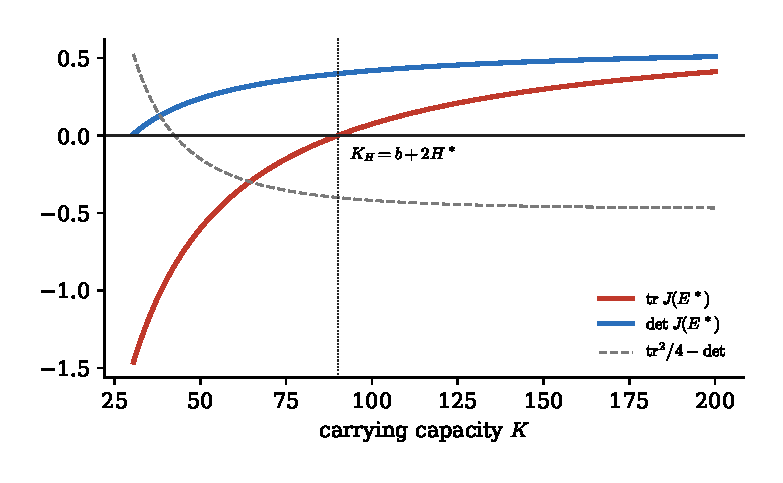
\includegraphics[width=0.7\linewidth]{joel_trace_det}
\caption{Trace and determinant of $J(E^*)$ as functions of $K$ (illustrative parameters).
The determinant stays positive for all feasible $K>H^*=30$, while the trace changes sign at
$K_H=90$. The dashed curve is negative (focus) for $K>42.5$.}
\label{fig:trace-det}
\end{figure}

% ---------------------------------------------------------------------
\subsection{The paradox of enrichment}

Increasing $K$ (enriching the hares' environment) leaves $H^*$ unchanged and only raises $P^*$:
every extra unit of carrying capacity is passed to the predator. Graphically, the prey parabola's
hump $(K-b)/2$ moves right while the predator nullcline stays at $H^*$, so for large enough $K$
the intersection falls left of the hump and the equilibrium destabilises. Past $K_H$ the system
settles on a limit cycle whose amplitude grows with $K$. For our illustrative parameters, at
$K=150$ the hare minimum on the cycle is about $1.1$ thousand, compared with $H^*=30$. In a
finite, stochastic population such deep troughs bring a real risk of extinction. Enrichment
thus \emph{destabilises} the system, the paradox named by Rosenzweig~\cite{rosenzweig1971}.

The mechanism is the saturating Holling type II response. At low $H$ each lynx's consumption
rises almost linearly with prey, which damps fluctuations; near and above $b$ it saturates, so
per-capita predation risk $aP/(b+H)$ \emph{falls} as hares increase. That positive feedback on
prey growth is exactly the term making $J_{11}>0$ left of the hump.

\paragraph{Link to Lotka--Volterra.} In the classical model ($K=\infty$, linear response) the
analogous Jacobian at coexistence has $\tau\equiv0$ for every parameter value, so it sits
permanently on the Hopf boundary. That is why its neutral cycles are structurally unstable: any
small change in the model's form moves it to one side or the other.
Rosenzweig--MacArthur makes the side explicit through the sign of $K-K_H$.

% ---------------------------------------------------------------------
\subsection{Illustrative regimes and numerical validation targets}\label{sec:joel-regimes}

These parameters are \emph{illustrative, not fitted}: $H$ and $P$ in thousands of pelts, $t$ in
years, with $r=1.5,\ a=4,\ b=30,\ e=0.4,\ m=0.8$. Then $ea=1.6=2m$, so $H^*=b=30$, $K_H=90$,
$\omega_0=\sqrt{0.4}\approx0.632$ and $T_0\approx9.94$ years, close to the observed decadal
cycle. Table~\ref{tab:joel-regimes} gives the expected behaviour on each side of the threshold;
the simulation section reproduces these with RK45 (\texttt{rtol}$=10^{-10}$,
\texttt{atol}$=10^{-12}$, 3000-year burn-in, start $(20,5)$).

\begin{table}[ht]
\centering
\small
\caption{Regimes in $K$ (other parameters fixed). Eigenvalues are of $J(E^*)$, except in A where
they are of $J(E_1)$.}
\label{tab:joel-regimes}
\setlength{\tabcolsep}{4pt}
\begin{tabular}{@{}cr l l l@{}}
\toprule
 & $K$ & Linear prediction & Eigenvalues & Long-run behaviour (simulated)\\
\midrule
A & 25  & $E^*$ infeasible ($K<H^*$) & $-1.5,\ -0.073$ & lynx die out; $\to(25,0)$\\
B & 60  & $E^*$ stable focus & $-0.188\pm0.515i$ & $\to(30,\,11.25)$, e-fold $\approx5$ yr\\
C & 85  & just below $K_H$ & $-0.022\pm0.623i$ & $\to(30,\,14.56)$, e-fold $\approx45$ yr\\
D & 90  & Hopf point & $\pm0.632i$ & very slow (algebraic) decay\\
E & 95  & just above $K_H$ & $+0.020\pm0.640i$ & cycle: $H\in[15.8,50.9]$, $P\in[9.8,20.8]$, $T=10.25$\\
F & 150 & well above $K_H$ & $+0.150\pm0.676i$ & cycle: $H\in[1.1,134.3]$, $P\in[1.7,41.2]$, $T=13.91$\\
\bottomrule
\end{tabular}
\end{table}

\noindent Two cautions for the numerics. At D the equilibrium is a weak focus ($\ell_1<0$), so
oscillations decay only like $t^{-1/2}$; after 3000 years the residual amplitude in $H$ is still
about $1.5$, which is expected and is not a sign of a cycle. The cycle at E is already large
because the amplitude coefficient is large ($A_H\approx7.8\sqrt{K-K_H}$), so ``small
amplitude'' only holds within about one unit of $K_H$.

\begin{figure}[ht]
\centering
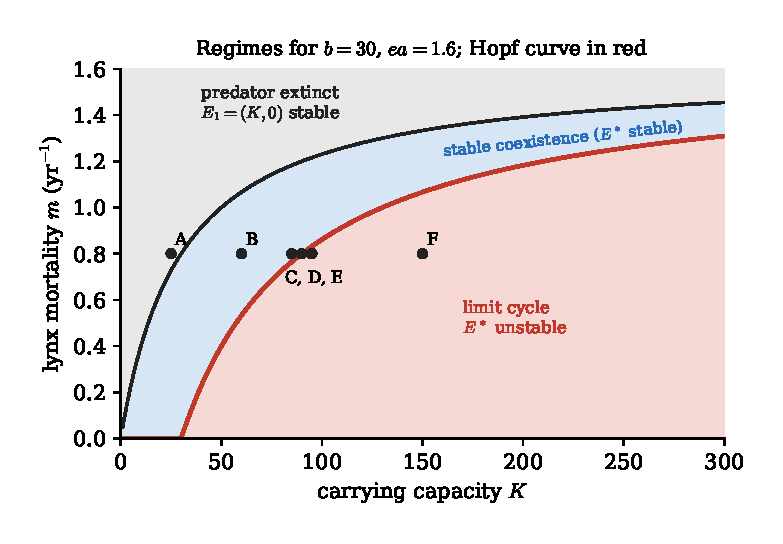
\includegraphics[width=0.7\linewidth]{joel_regions}
\caption{Analytic regimes in the $(K,m)$ plane for $b=30$, $ea=1.6$. Black curve:
$m=eaK/(b+K)$ (predator persistence boundary). Red curve: $m=ea(K-b)/(K+b)$ (Hopf curve).
Dots mark regimes A--F of Table~\ref{tab:joel-regimes}.}
\label{fig:regions}
\end{figure}

% ---------------------------------------------------------------------
\subsection{Sensitivity of the threshold}

Because $K_H=b(ea+m)/(ea-m)$ is explicit, sensitivity can be read off exactly. The elasticities
(percentage change in $K_H$ per percentage change in a parameter) are
\[
\frac{\partial\ln K_H}{\partial\ln b}=1,\qquad
\frac{\partial\ln K_H}{\partial\ln m}=-\frac{\partial\ln K_H}{\partial\ln a}
=-\frac{\partial\ln K_H}{\partial\ln e}=\frac{2\,ea\,m}{(ea)^2-m^2},\qquad
\frac{\partial\ln K_H}{\partial\ln r}=0.
\]
At the illustrative values ($ea=2m$) the middle elasticity is $4/3$: a 10\% rise in lynx
mortality raises the threshold by about 13\%, and so stabilises the system. The elasticity blows
up as $m\to ea$, where the predator is barely viable and $K_H\to\infty$. Weak predators stabilise.

Equivalently, for fixed $K$ the regimes are bands in $m$ (Figure~\ref{fig:regions}):
\[
\underbrace{m<\frac{ea(K-b)}{K+b}}_{\text{limit cycle}}
\qquad
\underbrace{\frac{ea(K-b)}{K+b}<m<\frac{eaK}{K+b}}_{\text{stable coexistence}}
\qquad
\underbrace{m>\frac{eaK}{K+b}}_{\text{lynx extinct}}
\]
A useful single number for any fitted parameter set is the \emph{stability margin}
$\sigma=K/K_H$, when coexistence is feasible: $\sigma<1$ gives a locally stable equilibrium (node or focus), while $\sigma>1$ gives an unstable equilibrium and the model's attracting cycle. Reporting
$\sigma$ (with its spread over fits) is the cleanest way to say whether the data support
sustained cycling.

For inference, $a$ and $e$ enter $H^*$ and $K_H$ through $ea$.
If an additional unknown predator observation scale is fitted, the transformation
$(P,a,e)\mapsto(cP,a/c,ec)$ introduces a scale ambiguity. In this historical iteration,
the observed pelt-state units are fixed and no scale factor is fitted, so this
transformation changes the observed predator values and does not by itself prove
non-identifiability of the effective coefficients. All six are fitted. Their practical
uncertainty is assessed using training diagnostics and the declared sensitivity runs,
and $a,e$ are not interpreted as uniquely recovered absolute biological rates.

% ---------------------------------------------------------------------
\subsection{Dimensionless form of the results}

With the scaling $x=H/K$, $y=aP/(rK)$, $s=rt$ (to be reconciled with the frozen scaling in the
model section), \eqref{eq:rm} becomes
\[
x'=x(1-x)-\frac{xy}{\beta+x},\qquad y'=y\Bigl(\frac{\alpha x}{\beta+x}-\delta\Bigr),
\qquad \beta=\frac{b}{K},\ \alpha=\frac{ea}{r},\ \delta=\frac{m}{r}.
\]
Then $x^*=\beta\delta/(\alpha-\delta)$, coexistence requires $\alpha>\delta$ and $x^*<1$, and the
Hopf condition $K=K_H$ reads $\beta(\alpha+\delta)/(\alpha-\delta)=1$, i.e.\ $\beta+2x^*=1$.
Only three combinations of the six parameters control the qualitative dynamics.

% ---------------------------------------------------------------------
\begin{table}[ht]
\centering
\small
\caption{Status of each stability claim in this section.}
\label{tab:joel-evidence}
\begin{tabular}{@{}p{0.52\linewidth}p{0.42\linewidth}@{}}
\toprule
Claim & Evidence \\
\midrule
Equilibria, feasibility, local stability of $E_0,E_1,E^*$ & Derived here; SymPy-checked\\
Hopf threshold $K_H=b+2H^*$, $\Delta>0$, transversality & Derived here; SymPy-checked\\
A periodic orbit exists for every $K>K_H$ & Derived here (Poincar\'e--Bendixson)\\
Cycle is unique and attracting for $K>K_H$ & Cited theorem~\cite{cheng1981}\\
$E^*$ globally stable for $H^*<K<K_H$ & Cited theorem~\cite{hsu1978}\\
Supercritical Hopf ($\ell_1<0$) & Numerical evaluation of analytic formula, two parameter sets\\
$\sqrt{K-K_H}$ amplitude law; periods, amplitudes, lags & Numerical (RK45), illustrative parameters\\
Real hare--lynx data lie on a limit cycle & \emph{Not established here}; requires $\sigma>1$ at fitted values with uncertainty\\
\bottomrule
\end{tabular}
\end{table}
\clearpage
% =====================================================================
%  Section owner: Rishi -- Numerical simulations and visualisation
%  Drop-in file:  % =====================================================================
%  Section owner: Rishi -- Numerical simulations and visualisation
%  Drop-in file:  % =====================================================================
%  Section owner: Rishi -- Numerical simulations and visualisation
%  Drop-in file:  \input{rishi_simulation_section}   (standalone build: rishi_main.tex)
%  Needs: amsmath, amssymb, booktabs, graphicx (PDF companions are used under pdflatex)
%  Figures: graphs/rishi_*.{eps,pdf}
%  Regenerate: python scripts/rishi_simulations.py   (numbers: results/simulations/)
%              python scripts/rishi_historical_placement.py   (results/simulations/historical/)
%  Code: src/lynx_hare/simulation.py, src/lynx_hare/simulation_plots.py,
%        notebooks/rishi_simulations.ipynb
% =====================================================================

\section{Numerical Simulations}\label{sec:rishi}

Section~\ref{sec:joel} locates the Hopf threshold $K_H=b+2H^*$ analytically. Linearisation is,
however, a local statement about the equilibrium at a single parameter value. This section tests
those predictions numerically and measures what linear analysis cannot give: the long-run
behaviour away from $E^*$, the size and period of the cycle, and the shape of the bifurcation.
Every trajectory is computed with the group's shared right-hand side of~\eqref{eq:rm}.

\subsection{Method}

\paragraph{Parameters.} We use the illustrative, unfitted values of Section~\ref{sec:joel}:
$r=1.5$, $a=4$, $b=30$, $e=0.4$, $m=0.8$ ($H,P$ in thousands of pelts, $t$ in years), for which
$H^*=30$, $K_H=90$ and $T_0=2\pi/\omega_0\approx 9.94$ years. The carrying capacity $K$ is varied.

\paragraph{Solver.} Equations~\eqref{eq:rm} are integrated with the adaptive Dormand--Prince
Runge--Kutta pair (RK45) in \texttt{scipy.integrate.solve\_ivp}~\cite{dormand1980,scipysolve}.
At each step a fourth- and a fifth-order estimate are formed from the same seven slope
evaluations; their difference estimates the local error, and the step is rejected and reduced
whenever this exceeds $\texttt{rtol}\,|y|+\texttt{atol}$. The project uses two settings of this
solver for two different jobs. Fitting and the 1900--1920 forecasts of the historical sections use
\texttt{model.solve} with $\texttt{rtol}=10^{-8}$, $\texttt{atol}=10^{-10}$ and a maximum step of
$0.1$ years, identical for both fitting methods. The long-run simulations in this section run for
thousands of years, so they use tighter tolerances, $\texttt{rtol}=10^{-10}$ and
$\texttt{atol}=10^{-12}$, without a step cap. Both call the same shared right-hand side. The
illustrative runs start from $(H_0,P_0)=(20,5)$; all values are in
\texttt{configs/simulations.json}.

\paragraph{Long-run behaviour.} To describe the attractor we integrate for a burn-in period
$T_{\mathrm{burn}}$, discard it, and record the next 300--400 years. On the recorded window we
report the range of $H$ and $P$; if $H$ still oscillates, the period is the mean interval between
successive hare maxima and the lag is the mean delay from a hare maximum to the next lynx
maximum. We take $T_{\mathrm{burn}}=3000$ years, increased to $20{,}000$ years when
$|K-K_H|<1$, where the equilibrium is a weak focus and transients decay very slowly.

\subsection{Solver accuracy}

The classical Lotka--Volterra system $\dot H=\alpha H-\beta HP$, $\dot P=\delta HP-\gamma P$
conserves $V=\delta H-\gamma\ln H+\beta P-\alpha\ln P$, so any drift in $V$ along a computed
orbit is numerical error. Over 100 time units RK45 keeps $|V(t)-V(0)|$ below $4\times10^{-10}$,
whereas explicit Euler with step $h=0.01$ drifts by $0.15$ and its orbit spirals outward
(Figure~\ref{fig:rishi_solver}), creating oscillatory growth the model does not have. For
Rosenzweig--MacArthur at $K=150$, tightening both tolerances a hundredfold changes the
solution by a relative $8\times10^{-10}$, and all states remain positive, as Lemma~\ref{lem:bounded}
requires.

\begin{figure}[htbp]
  \centering
  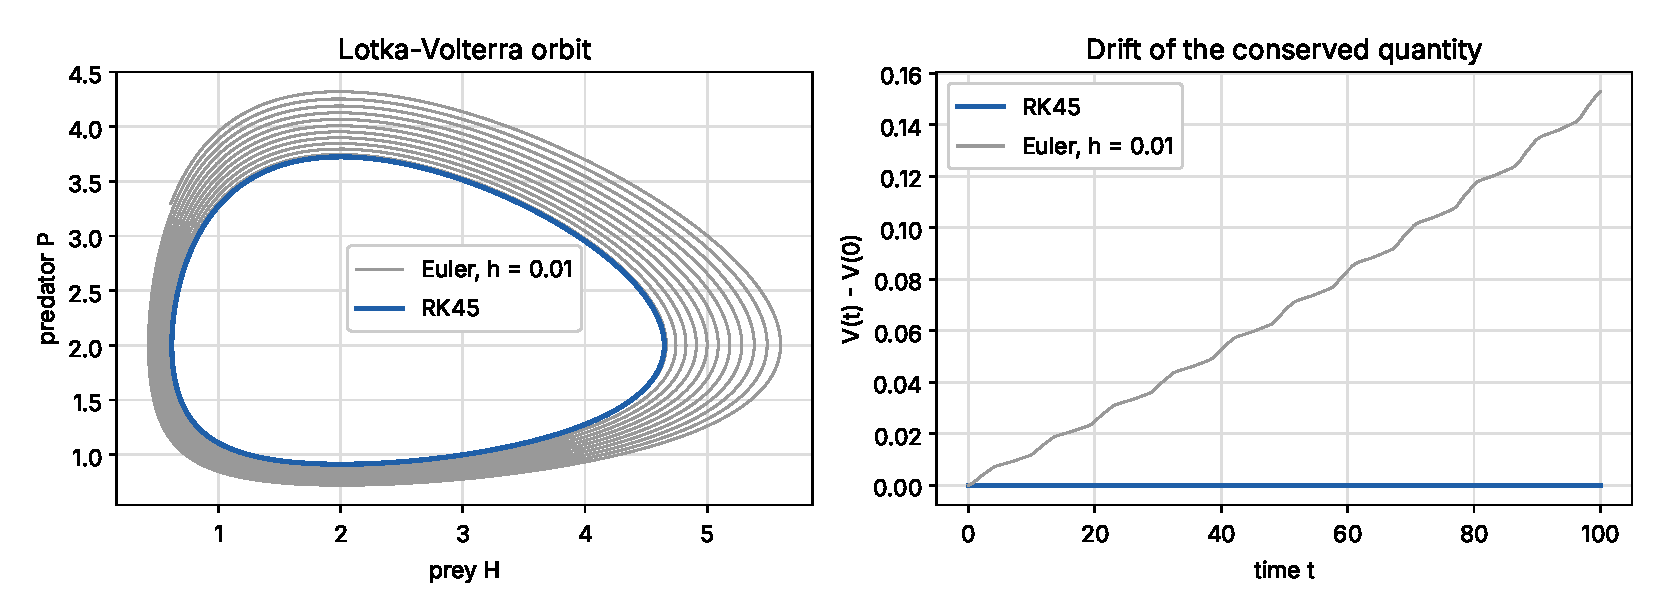
\includegraphics[width=0.9\linewidth]{rishi_solver_validation}
  \caption{Solver check on Lotka--Volterra. RK45 preserves the conserved quantity $V$ and
  closes the orbit; Euler ($h=0.01$) drifts and spirals outward. Only an accurate solver can
  distinguish a genuine limit cycle from a numerical artefact.}
  \label{fig:rishi_solver}
\end{figure}

\subsection{Reproduction of the analytic regimes}

Table~\ref{tab:rishi_regimes} reproduces each validation target of Section~\ref{sec:joel}
(3000-year burn-in throughout). Regime~D lies exactly on $K_H$: the residual oscillation there is
a slowly decaying transient (decay is only algebraic at a weak focus), not a cycle.

\begin{table}[htbp]
  \centering
  \caption{Simulated long-run behaviour for the regimes of Section~\ref{sec:joel}. Ranges are
  over 400 years after the burn-in; period and lynx lag are in years.}
  \label{tab:rishi_regimes}
  \begin{tabular}{clccccc}
    \toprule
    & $K$ & Eigenvalues & $H$ range & $P$ range & Period & Lag \\
    \midrule
    A & 25  & $-1.5,\ -0.073$ ($E_1$) & $25.0$         & $0$              & -- & -- \\
    B & 60  & $-0.188\pm0.515i$ & $30.0$         & $11.25$          & -- & -- \\
    C & 85  & $-0.022\pm0.623i$ & $30.0$         & $14.56$          & -- & -- \\
    D & 90  & $\pm0.632i$       & $[28.5,31.6]$  & $[14.51,15.49]$  & 9.94  & 2.50 \\
    E & 95  & $+0.020\pm0.640i$ & $[15.8,50.9]$  & $[9.81,20.75]$   & 10.25 & 2.81 \\
    F & 150 & $+0.150\pm0.676i$ & $[1.1,134.3]$  & $[1.69,41.16]$   & 13.91 & 4.52 \\
    \bottomrule
  \end{tabular}
\end{table}

Figure~\ref{fig:rishi_regimes} shows four of these regimes. Below the threshold (B, C) the
predator nullcline meets the prey hump to the right of its peak and trajectories spiral into
$E^*$; at $K=85$ the trace is only $-0.044$, so the decay takes centuries. Above the threshold
(E, F) the intersection lies left of the peak, $E^*$ repels, and the orbit settles onto a
sustained cycle that circulates counter-clockwise, with lynx peaks lagging hare peaks.

\begin{figure}[htbp]
  \centering
  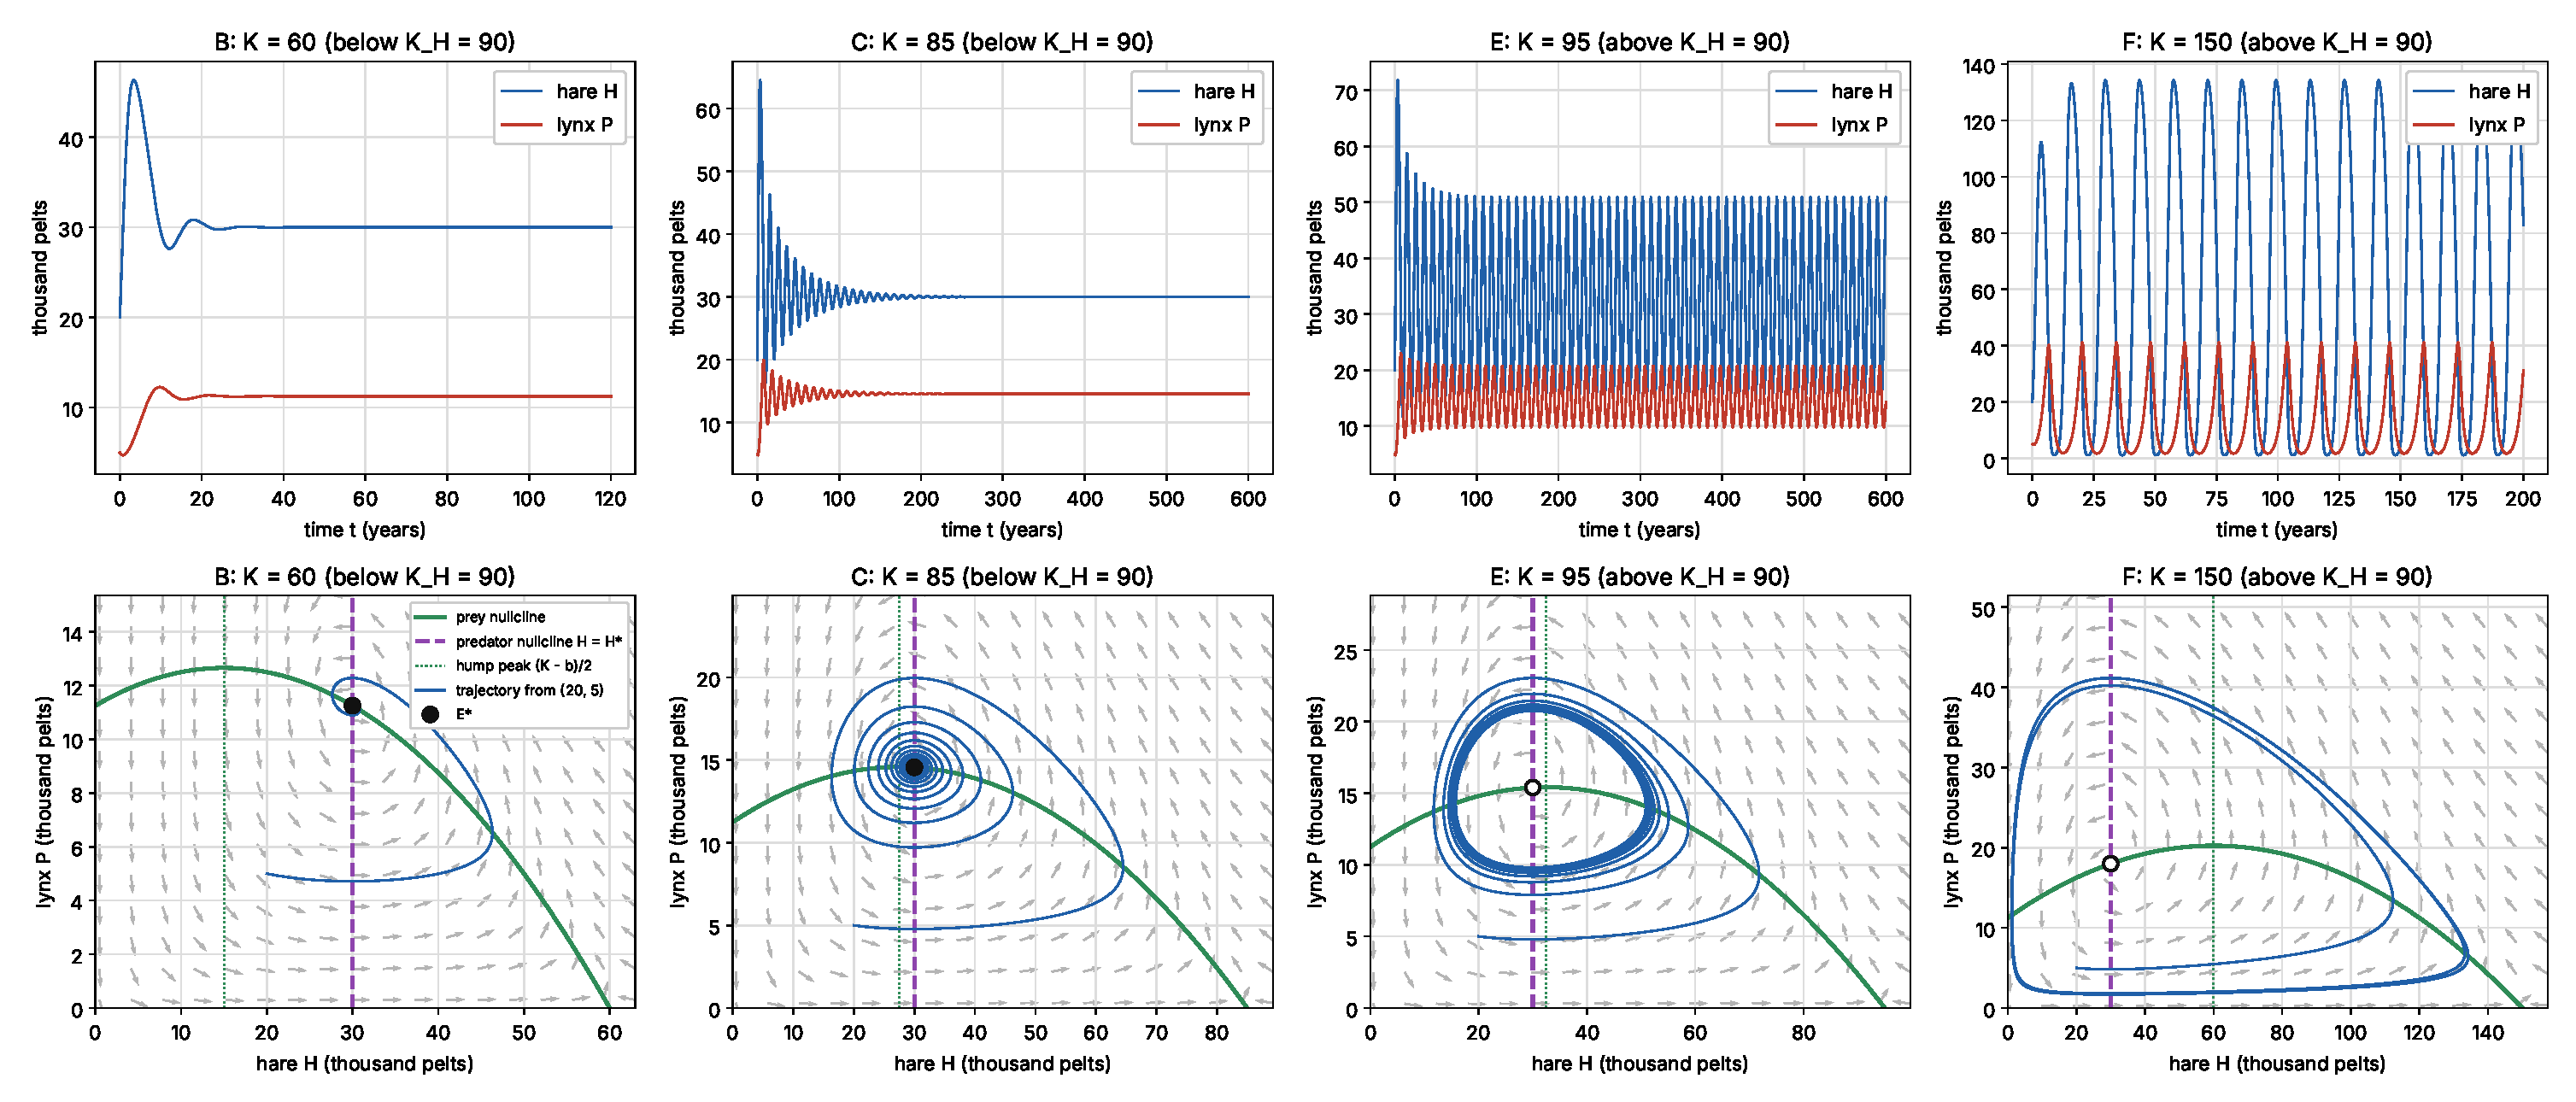
\includegraphics[width=\linewidth]{rishi_regimes}
  \caption{Time series (top) and phase portraits (bottom) from $(20,5)$ for $K=60,85$ (below
  $K_H=90$) and $K=95,150$ (above). Green: prey nullcline; dashed purple: predator nullcline
  $H=H^*$; dotted: hump peak $(K-b)/2$. Filled/open circle: stable/unstable $E^*$. Oscillations
  decay below $K_H$ and persist above it.}
  \label{fig:rishi_regimes}
\end{figure}

\subsection{The limit cycle attracts}

For Lotka--Volterra every initial condition lies on its own closed orbit. At $K=150$ we start one
trajectory beside the unstable equilibrium and one far outside the cycle
(Figure~\ref{fig:rishi_cycle}). The first spirals outward, the second inward, and their successive
hare maxima converge to the same value, $134.277$. The cycle is therefore orbitally stable,
in agreement with the uniqueness result cited in Section~\ref{sec:joel}~\cite{cheng1981}.

\begin{figure}[htbp]
  \centering
  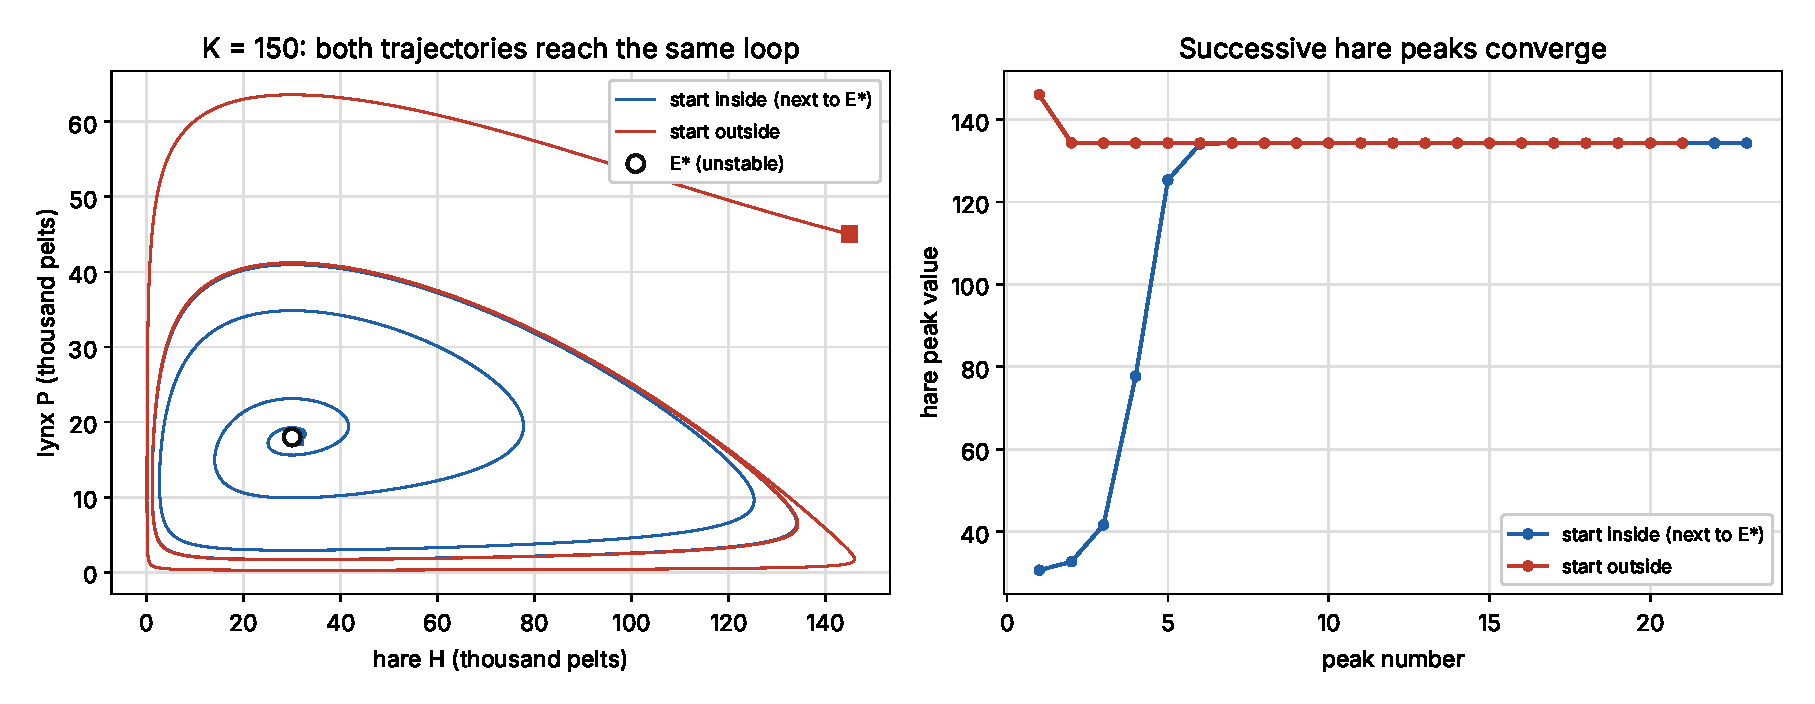
\includegraphics[width=0.9\linewidth]{rishi_limit_cycle}
  \caption{At $K=150$, trajectories started inside and outside the cycle converge onto the same
  closed orbit (left); their successive hare maxima approach a common value (right).}
  \label{fig:rishi_cycle}
\end{figure}

\subsection{Bifurcation in $K$}

Root-finding on the numerically evaluated trace of $J(E^*)$ places the sign change at
$K=90.0000000000$, in agreement with $K_H=b+2H^*$ and Figure~\ref{fig:trace-det}; there the
eigenvalues are $\pm0.632i=\pm i\omega_0$, and they become complex (node to focus) at $K\approx42.6$.

The numerical bifurcation diagram (Figure~\ref{fig:rishi_bif}) records the post-transient maximum
and minimum for 113 values of $K$ between 32 and 200. For $K<89$ the two coincide (largest
spread $5\times10^{-5}$): the solution settles on $E^*$. At $K_H$ the branches separate continuously
from the equilibrium and the cycle grows with $K$. Just above the threshold its half-amplitude
follows $A\approx7.8\sqrt{K-K_H}$, with fitted log--log slope $0.507$ for $0.5\le K-K_H\le8$
(Figure~\ref{fig:rishi_amp}), and the period approaches $T_0=9.93$ years ($9.97$ years at
$K-K_H=0.5$). This square-root growth from zero amplitude is the signature of a supercritical
Hopf bifurcation, consistent with the negative first Lyapunov coefficient of
Section~\ref{sec:joel}. As $K$ increases further the cycle minima approach zero: at $K=200$ the
hare minimum is $0.12$ thousand pelts, the paradox of enrichment~\cite{rosenzweig1971}.

\begin{figure}[htbp]
  \centering
  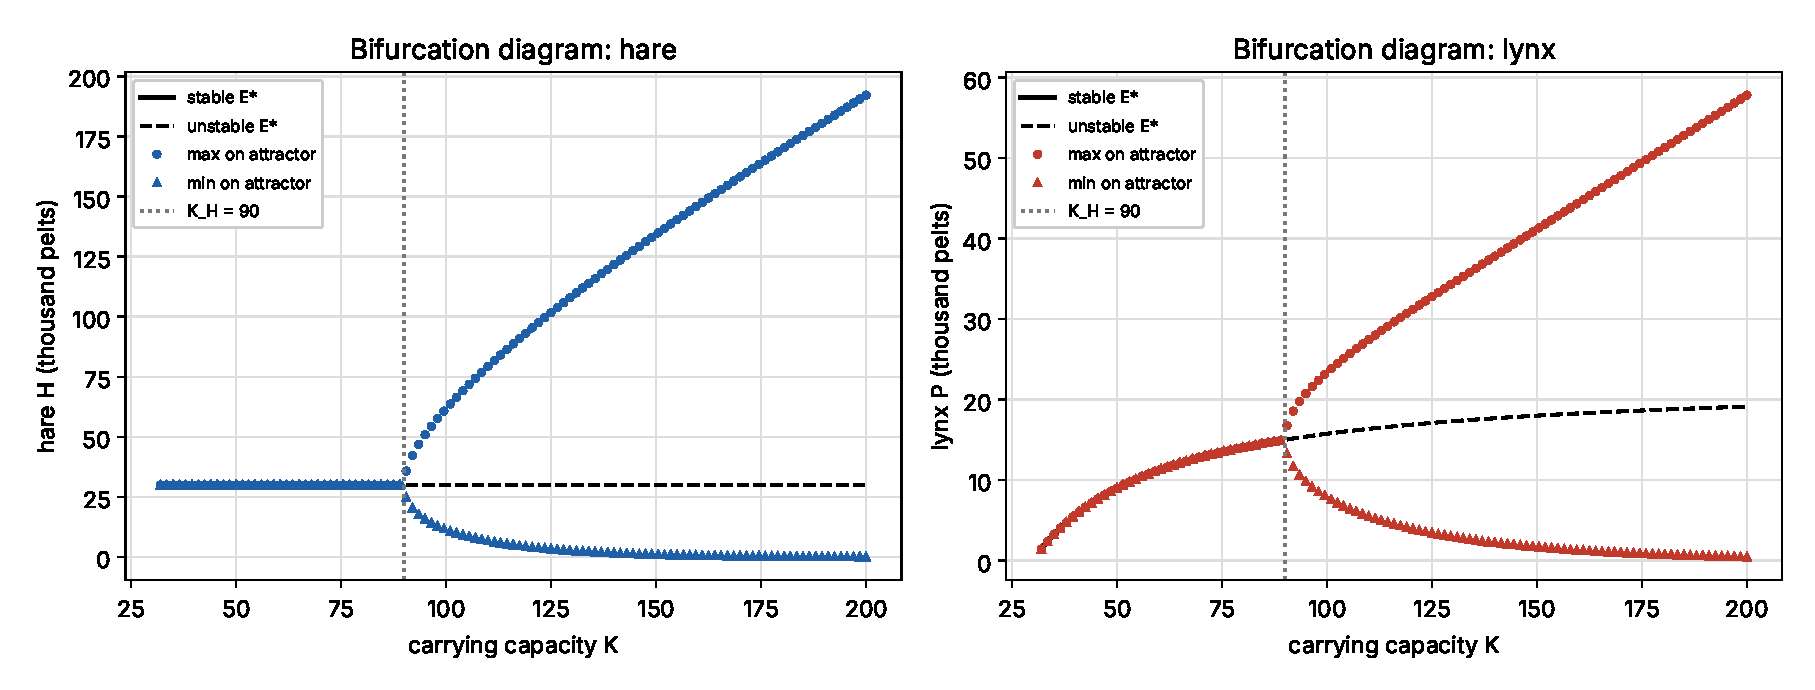
\includegraphics[width=0.9\linewidth]{rishi_bifurcation}
  \caption{Numerical bifurcation diagram: maximum and minimum of $H$ (left) and $P$ (right) after
  the burn-in, against $K$. Solid/dashed black: stable/unstable $E^*$. A cycle is born at
  $K_H=90$ with zero amplitude and its minima approach zero as $K$ grows.}
  \label{fig:rishi_bif}
\end{figure}

\begin{figure}[htbp]
  \centering
  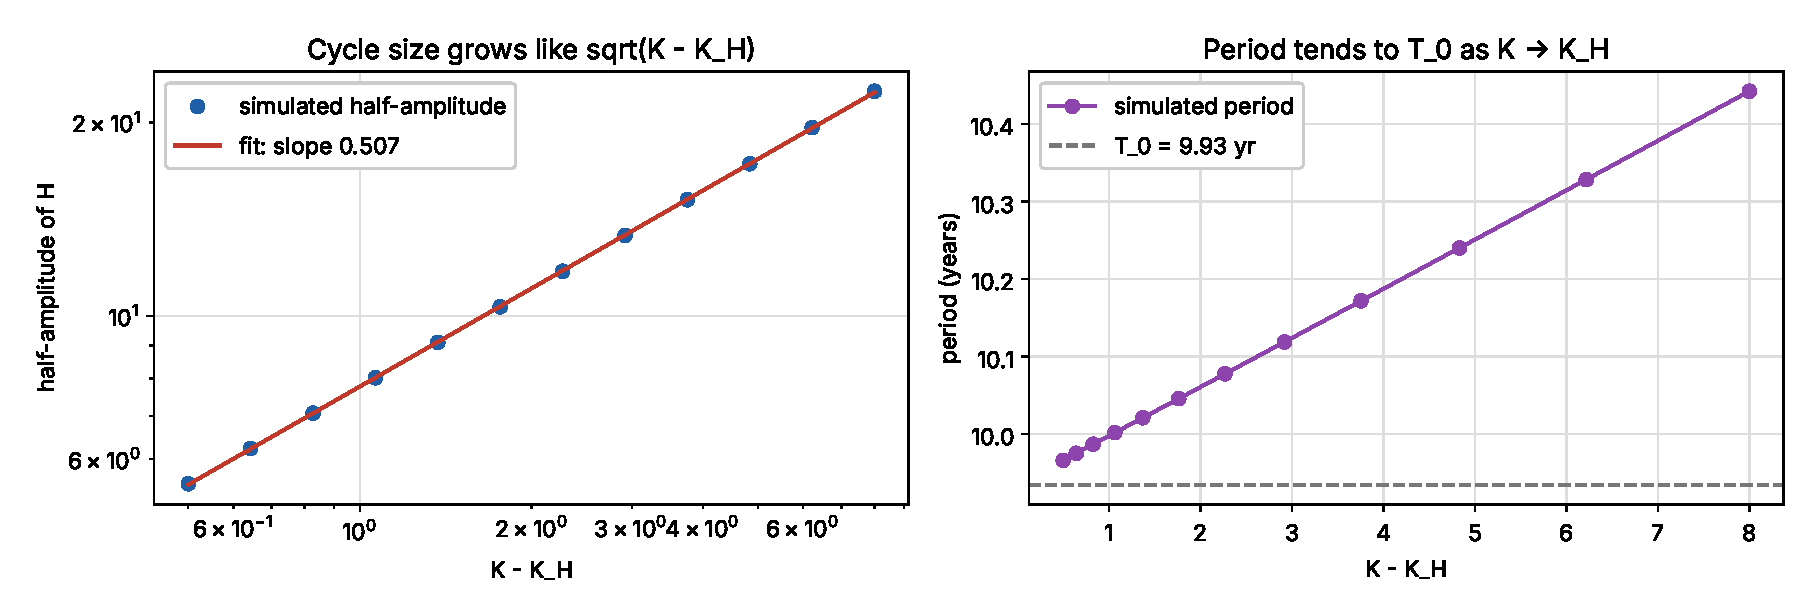
\includegraphics[width=0.9\linewidth]{rishi_amplitude_period}
  \caption{Left: half-amplitude of $H$ against $K-K_H$ on log--log axes, with slope $0.507$
  (supercritical prediction $1/2$). Right: cycle period, tending to $T_0=2\pi/\omega_0$.}
  \label{fig:rishi_amp}
\end{figure}

\subsection{Scope}

These simulations use illustrative, unfitted parameters and provide numerical evidence for one
parameter set, not proofs. Near $K_H$ the results depend on the burn-in length, which is why it
is lengthened there. Whether the historical hare--lynx series lies above or below the threshold
depends on $\sigma=K/K_H$ at the fitted parameters and is addressed in the fitting sections.
   (standalone build: rishi_main.tex)
%  Needs: amsmath, amssymb, booktabs, graphicx (PDF companions are used under pdflatex)
%  Figures: graphs/rishi_*.{eps,pdf}
%  Regenerate: python scripts/rishi_simulations.py   (numbers: results/simulations/)
%              python scripts/rishi_historical_placement.py   (results/simulations/historical/)
%  Code: src/lynx_hare/simulation.py, src/lynx_hare/simulation_plots.py,
%        notebooks/rishi_simulations.ipynb
% =====================================================================

\section{Numerical Simulations}\label{sec:rishi}

Section~\ref{sec:joel} locates the Hopf threshold $K_H=b+2H^*$ analytically. Linearisation is,
however, a local statement about the equilibrium at a single parameter value. This section tests
those predictions numerically and measures what linear analysis cannot give: the long-run
behaviour away from $E^*$, the size and period of the cycle, and the shape of the bifurcation.
Every trajectory is computed with the group's shared right-hand side of~\eqref{eq:rm}.

\subsection{Method}

\paragraph{Parameters.} We use the illustrative, unfitted values of Section~\ref{sec:joel}:
$r=1.5$, $a=4$, $b=30$, $e=0.4$, $m=0.8$ ($H,P$ in thousands of pelts, $t$ in years), for which
$H^*=30$, $K_H=90$ and $T_0=2\pi/\omega_0\approx 9.94$ years. The carrying capacity $K$ is varied.

\paragraph{Solver.} Equations~\eqref{eq:rm} are integrated with the adaptive Dormand--Prince
Runge--Kutta pair (RK45) in \texttt{scipy.integrate.solve\_ivp}~\cite{dormand1980,scipysolve}.
At each step a fourth- and a fifth-order estimate are formed from the same seven slope
evaluations; their difference estimates the local error, and the step is rejected and reduced
whenever this exceeds $\texttt{rtol}\,|y|+\texttt{atol}$. The project uses two settings of this
solver for two different jobs. Fitting and the 1900--1920 forecasts of the historical sections use
\texttt{model.solve} with $\texttt{rtol}=10^{-8}$, $\texttt{atol}=10^{-10}$ and a maximum step of
$0.1$ years, identical for both fitting methods. The long-run simulations in this section run for
thousands of years, so they use tighter tolerances, $\texttt{rtol}=10^{-10}$ and
$\texttt{atol}=10^{-12}$, without a step cap. Both call the same shared right-hand side. The
illustrative runs start from $(H_0,P_0)=(20,5)$; all values are in
\texttt{configs/simulations.json}.

\paragraph{Long-run behaviour.} To describe the attractor we integrate for a burn-in period
$T_{\mathrm{burn}}$, discard it, and record the next 300--400 years. On the recorded window we
report the range of $H$ and $P$; if $H$ still oscillates, the period is the mean interval between
successive hare maxima and the lag is the mean delay from a hare maximum to the next lynx
maximum. We take $T_{\mathrm{burn}}=3000$ years, increased to $20{,}000$ years when
$|K-K_H|<1$, where the equilibrium is a weak focus and transients decay very slowly.

\subsection{Solver accuracy}

The classical Lotka--Volterra system $\dot H=\alpha H-\beta HP$, $\dot P=\delta HP-\gamma P$
conserves $V=\delta H-\gamma\ln H+\beta P-\alpha\ln P$, so any drift in $V$ along a computed
orbit is numerical error. Over 100 time units RK45 keeps $|V(t)-V(0)|$ below $4\times10^{-10}$,
whereas explicit Euler with step $h=0.01$ drifts by $0.15$ and its orbit spirals outward
(Figure~\ref{fig:rishi_solver}), creating oscillatory growth the model does not have. For
Rosenzweig--MacArthur at $K=150$, tightening both tolerances a hundredfold changes the
solution by a relative $8\times10^{-10}$, and all states remain positive, as Lemma~\ref{lem:bounded}
requires.

\begin{figure}[htbp]
  \centering
  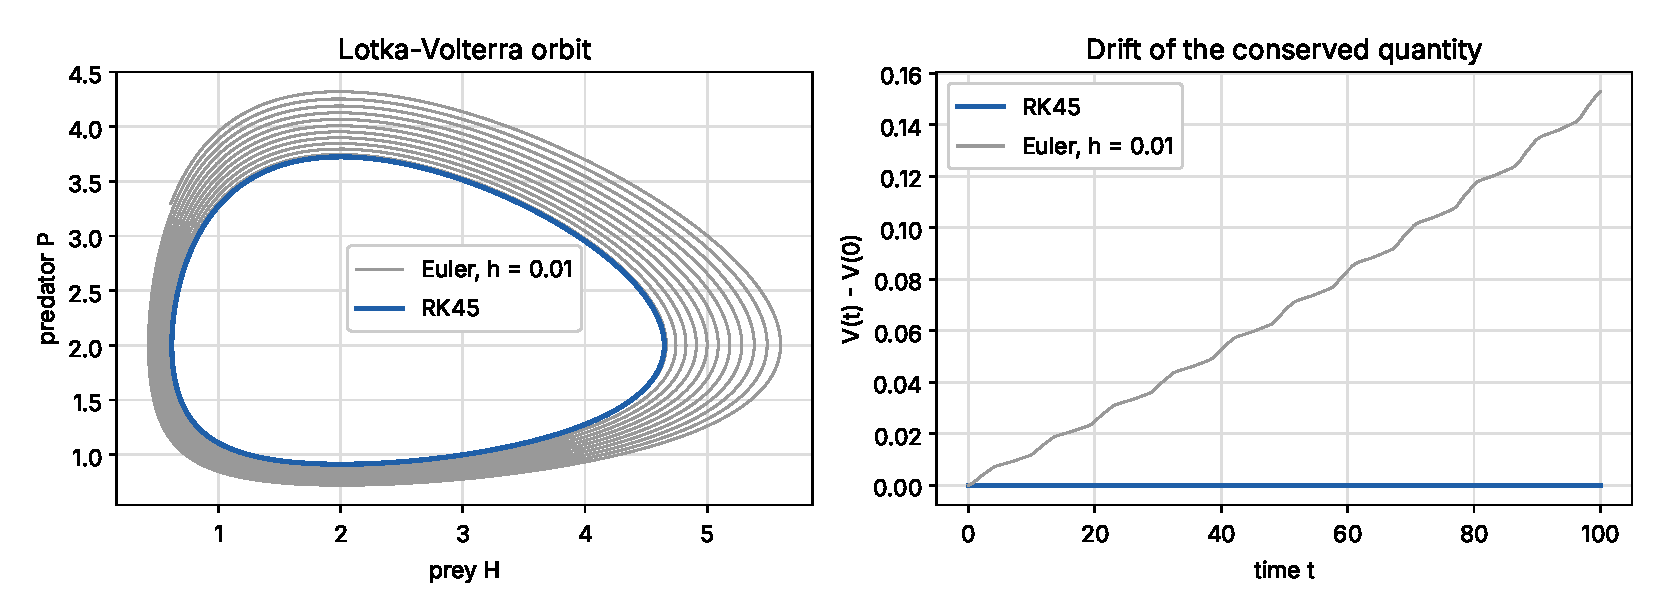
\includegraphics[width=0.9\linewidth]{rishi_solver_validation}
  \caption{Solver check on Lotka--Volterra. RK45 preserves the conserved quantity $V$ and
  closes the orbit; Euler ($h=0.01$) drifts and spirals outward. Only an accurate solver can
  distinguish a genuine limit cycle from a numerical artefact.}
  \label{fig:rishi_solver}
\end{figure}

\subsection{Reproduction of the analytic regimes}

Table~\ref{tab:rishi_regimes} reproduces each validation target of Section~\ref{sec:joel}
(3000-year burn-in throughout). Regime~D lies exactly on $K_H$: the residual oscillation there is
a slowly decaying transient (decay is only algebraic at a weak focus), not a cycle.

\begin{table}[htbp]
  \centering
  \caption{Simulated long-run behaviour for the regimes of Section~\ref{sec:joel}. Ranges are
  over 400 years after the burn-in; period and lynx lag are in years.}
  \label{tab:rishi_regimes}
  \begin{tabular}{clccccc}
    \toprule
    & $K$ & Eigenvalues & $H$ range & $P$ range & Period & Lag \\
    \midrule
    A & 25  & $-1.5,\ -0.073$ ($E_1$) & $25.0$         & $0$              & -- & -- \\
    B & 60  & $-0.188\pm0.515i$ & $30.0$         & $11.25$          & -- & -- \\
    C & 85  & $-0.022\pm0.623i$ & $30.0$         & $14.56$          & -- & -- \\
    D & 90  & $\pm0.632i$       & $[28.5,31.6]$  & $[14.51,15.49]$  & 9.94  & 2.50 \\
    E & 95  & $+0.020\pm0.640i$ & $[15.8,50.9]$  & $[9.81,20.75]$   & 10.25 & 2.81 \\
    F & 150 & $+0.150\pm0.676i$ & $[1.1,134.3]$  & $[1.69,41.16]$   & 13.91 & 4.52 \\
    \bottomrule
  \end{tabular}
\end{table}

Figure~\ref{fig:rishi_regimes} shows four of these regimes. Below the threshold (B, C) the
predator nullcline meets the prey hump to the right of its peak and trajectories spiral into
$E^*$; at $K=85$ the trace is only $-0.044$, so the decay takes centuries. Above the threshold
(E, F) the intersection lies left of the peak, $E^*$ repels, and the orbit settles onto a
sustained cycle that circulates counter-clockwise, with lynx peaks lagging hare peaks.

\begin{figure}[htbp]
  \centering
  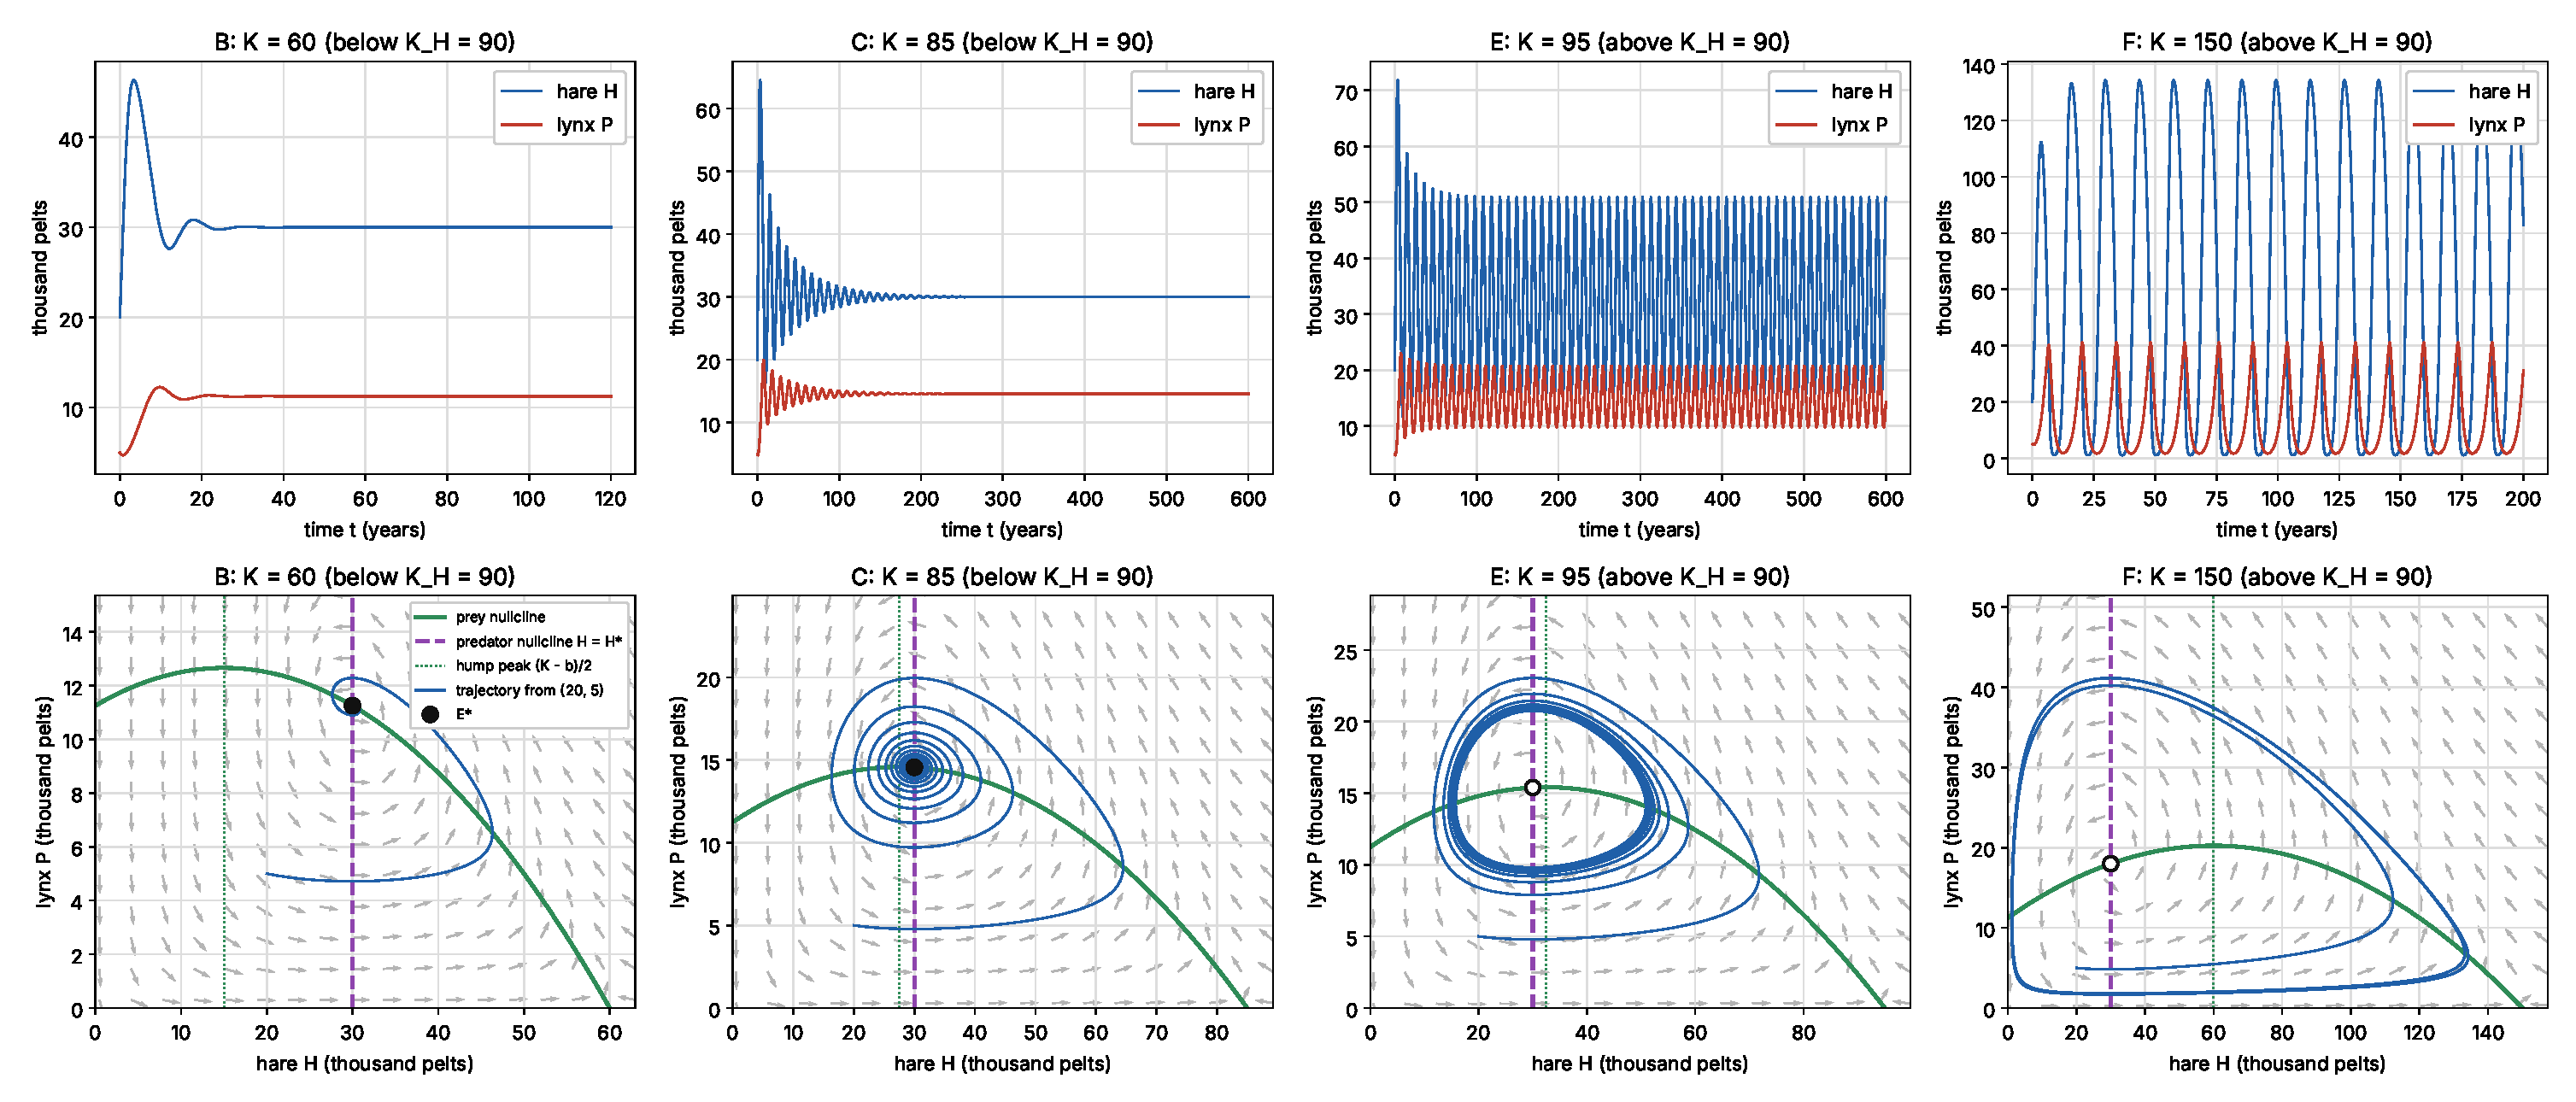
\includegraphics[width=\linewidth]{rishi_regimes}
  \caption{Time series (top) and phase portraits (bottom) from $(20,5)$ for $K=60,85$ (below
  $K_H=90$) and $K=95,150$ (above). Green: prey nullcline; dashed purple: predator nullcline
  $H=H^*$; dotted: hump peak $(K-b)/2$. Filled/open circle: stable/unstable $E^*$. Oscillations
  decay below $K_H$ and persist above it.}
  \label{fig:rishi_regimes}
\end{figure}

\subsection{The limit cycle attracts}

For Lotka--Volterra every initial condition lies on its own closed orbit. At $K=150$ we start one
trajectory beside the unstable equilibrium and one far outside the cycle
(Figure~\ref{fig:rishi_cycle}). The first spirals outward, the second inward, and their successive
hare maxima converge to the same value, $134.277$. The cycle is therefore orbitally stable,
in agreement with the uniqueness result cited in Section~\ref{sec:joel}~\cite{cheng1981}.

\begin{figure}[htbp]
  \centering
  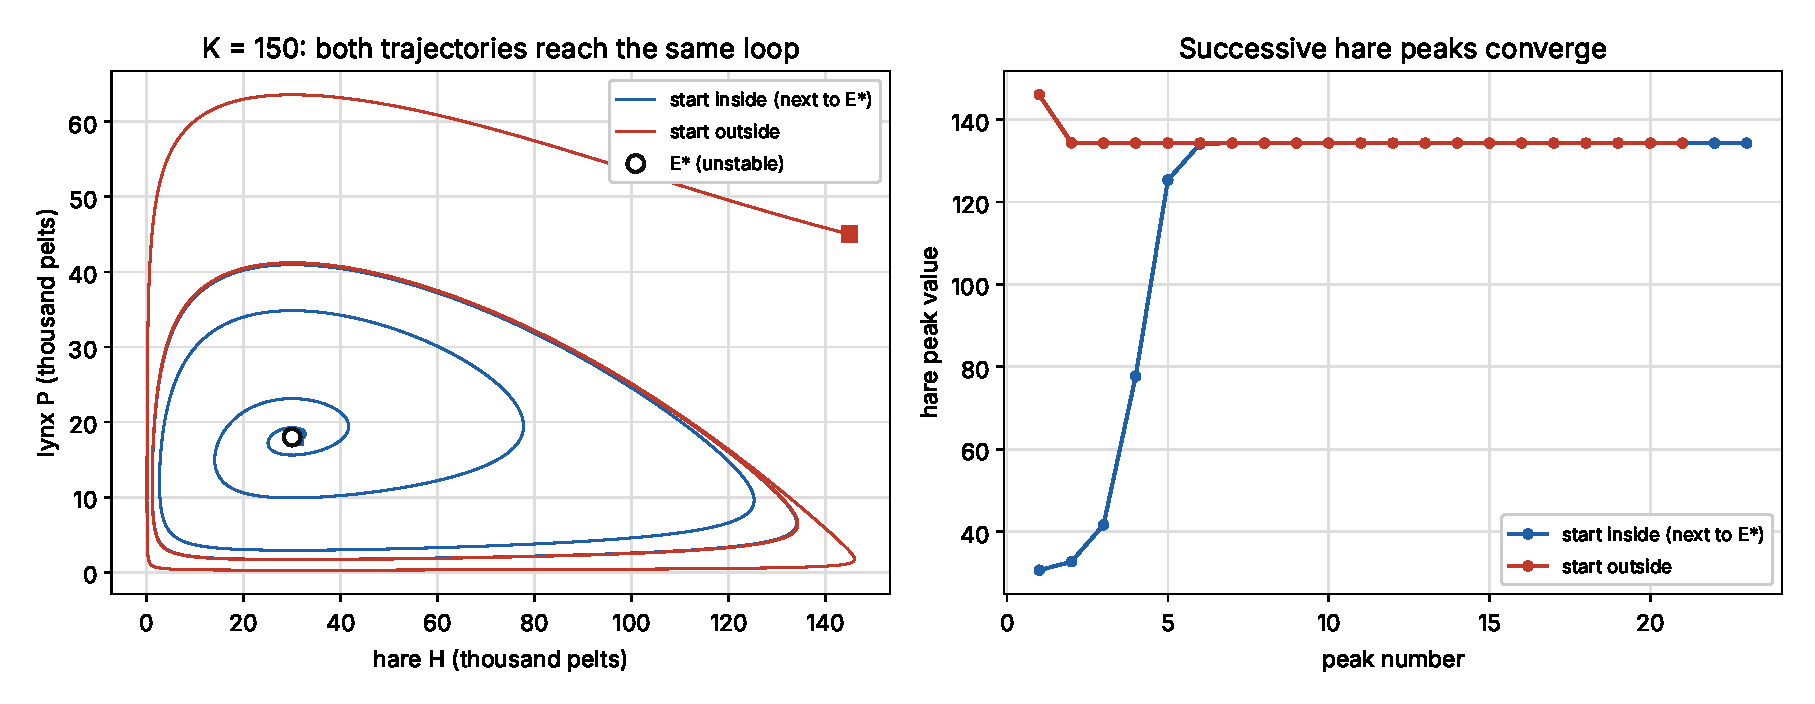
\includegraphics[width=0.9\linewidth]{rishi_limit_cycle}
  \caption{At $K=150$, trajectories started inside and outside the cycle converge onto the same
  closed orbit (left); their successive hare maxima approach a common value (right).}
  \label{fig:rishi_cycle}
\end{figure}

\subsection{Bifurcation in $K$}

Root-finding on the numerically evaluated trace of $J(E^*)$ places the sign change at
$K=90.0000000000$, in agreement with $K_H=b+2H^*$ and Figure~\ref{fig:trace-det}; there the
eigenvalues are $\pm0.632i=\pm i\omega_0$, and they become complex (node to focus) at $K\approx42.6$.

The numerical bifurcation diagram (Figure~\ref{fig:rishi_bif}) records the post-transient maximum
and minimum for 113 values of $K$ between 32 and 200. For $K<89$ the two coincide (largest
spread $5\times10^{-5}$): the solution settles on $E^*$. At $K_H$ the branches separate continuously
from the equilibrium and the cycle grows with $K$. Just above the threshold its half-amplitude
follows $A\approx7.8\sqrt{K-K_H}$, with fitted log--log slope $0.507$ for $0.5\le K-K_H\le8$
(Figure~\ref{fig:rishi_amp}), and the period approaches $T_0=9.93$ years ($9.97$ years at
$K-K_H=0.5$). This square-root growth from zero amplitude is the signature of a supercritical
Hopf bifurcation, consistent with the negative first Lyapunov coefficient of
Section~\ref{sec:joel}. As $K$ increases further the cycle minima approach zero: at $K=200$ the
hare minimum is $0.12$ thousand pelts, the paradox of enrichment~\cite{rosenzweig1971}.

\begin{figure}[htbp]
  \centering
  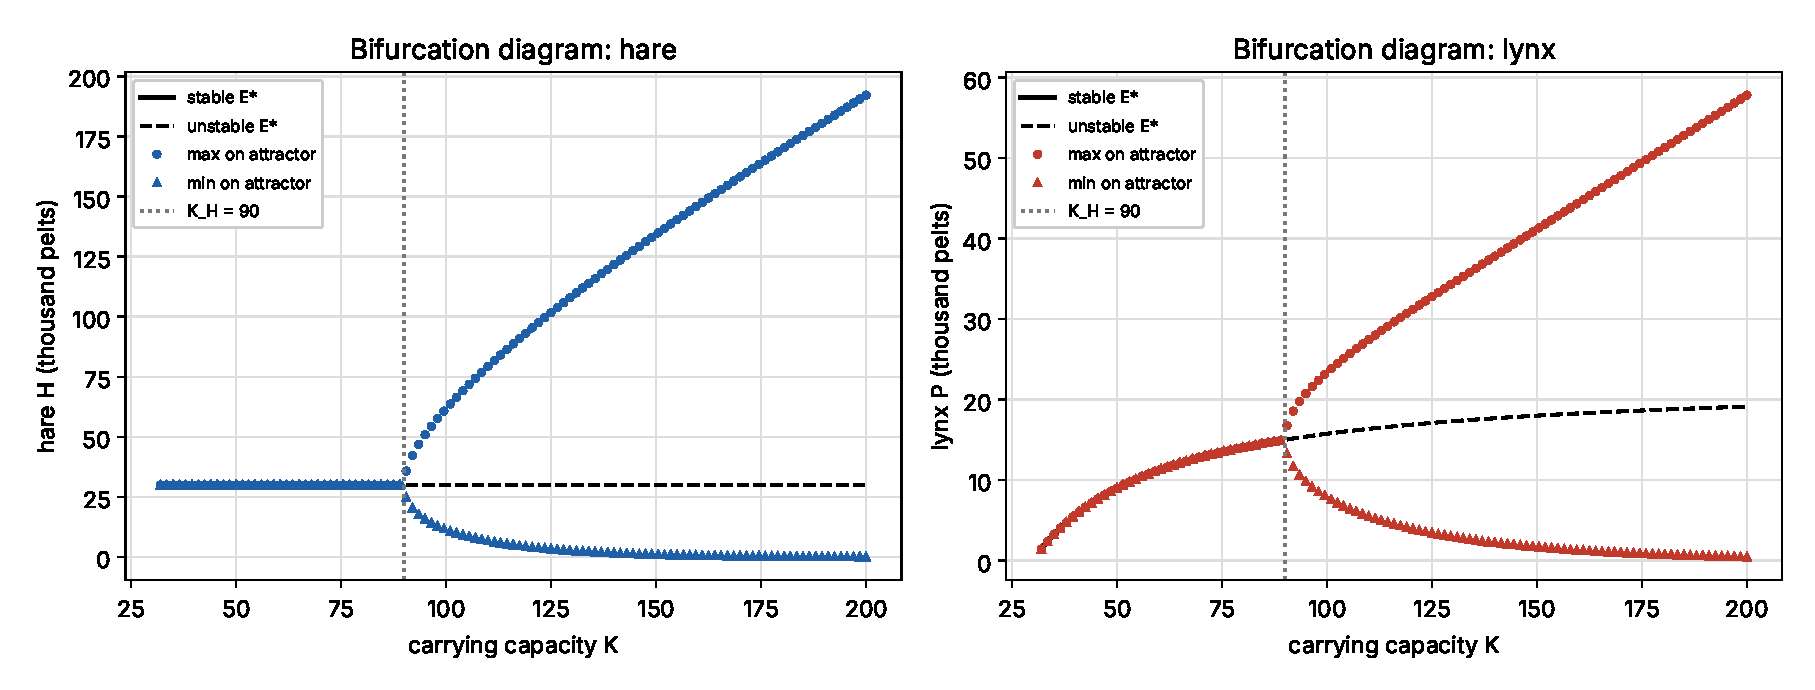
\includegraphics[width=0.9\linewidth]{rishi_bifurcation}
  \caption{Numerical bifurcation diagram: maximum and minimum of $H$ (left) and $P$ (right) after
  the burn-in, against $K$. Solid/dashed black: stable/unstable $E^*$. A cycle is born at
  $K_H=90$ with zero amplitude and its minima approach zero as $K$ grows.}
  \label{fig:rishi_bif}
\end{figure}

\begin{figure}[htbp]
  \centering
  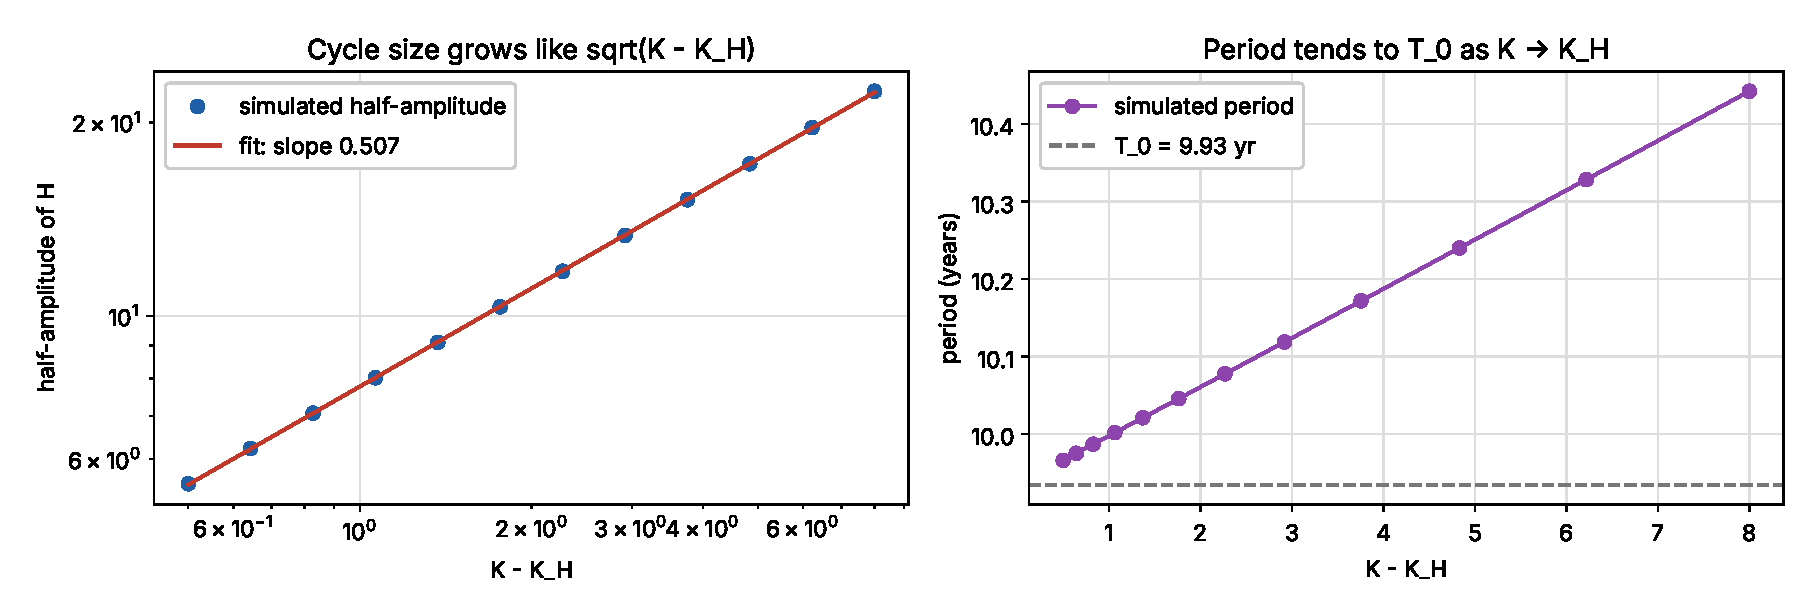
\includegraphics[width=0.9\linewidth]{rishi_amplitude_period}
  \caption{Left: half-amplitude of $H$ against $K-K_H$ on log--log axes, with slope $0.507$
  (supercritical prediction $1/2$). Right: cycle period, tending to $T_0=2\pi/\omega_0$.}
  \label{fig:rishi_amp}
\end{figure}

\subsection{Scope}

These simulations use illustrative, unfitted parameters and provide numerical evidence for one
parameter set, not proofs. Near $K_H$ the results depend on the burn-in length, which is why it
is lengthened there. Whether the historical hare--lynx series lies above or below the threshold
depends on $\sigma=K/K_H$ at the fitted parameters and is addressed in the fitting sections.
   (standalone build: rishi_main.tex)
%  Needs: amsmath, amssymb, booktabs, graphicx (PDF companions are used under pdflatex)
%  Figures: graphs/rishi_*.{eps,pdf}
%  Regenerate: python scripts/rishi_simulations.py   (numbers: results/simulations/)
%              python scripts/rishi_historical_placement.py   (results/simulations/historical/)
%  Code: src/lynx_hare/simulation.py, src/lynx_hare/simulation_plots.py,
%        notebooks/rishi_simulations.ipynb
% =====================================================================

\section{Numerical Simulations}\label{sec:rishi}

Section~\ref{sec:joel} locates the Hopf threshold $K_H=b+2H^*$ analytically. Linearisation is,
however, a local statement about the equilibrium at a single parameter value. This section tests
those predictions numerically and measures what linear analysis cannot give: the long-run
behaviour away from $E^*$, the size and period of the cycle, and the shape of the bifurcation.
Every trajectory is computed with the group's shared right-hand side of~\eqref{eq:rm}.

\subsection{Method}

\paragraph{Parameters.} We use the illustrative, unfitted values of Section~\ref{sec:joel}:
$r=1.5$, $a=4$, $b=30$, $e=0.4$, $m=0.8$ ($H,P$ in thousands of pelts, $t$ in years), for which
$H^*=30$, $K_H=90$ and $T_0=2\pi/\omega_0\approx 9.94$ years. The carrying capacity $K$ is varied.

\paragraph{Solver.} Equations~\eqref{eq:rm} are integrated with the adaptive Dormand--Prince
Runge--Kutta pair (RK45) in \texttt{scipy.integrate.solve\_ivp}~\cite{dormand1980,scipysolve}.
At each step a fourth- and a fifth-order estimate are formed from the same seven slope
evaluations; their difference estimates the local error, and the step is rejected and reduced
whenever this exceeds $\texttt{rtol}\,|y|+\texttt{atol}$. The project uses two settings of this
solver for two different jobs. Fitting and the 1900--1920 forecasts of the historical sections use
\texttt{model.solve} with $\texttt{rtol}=10^{-8}$, $\texttt{atol}=10^{-10}$ and a maximum step of
$0.1$ years, identical for both fitting methods. The long-run simulations in this section run for
thousands of years, so they use tighter tolerances, $\texttt{rtol}=10^{-10}$ and
$\texttt{atol}=10^{-12}$, without a step cap. Both call the same shared right-hand side. The
illustrative runs start from $(H_0,P_0)=(20,5)$; all values are in
\texttt{configs/simulations.json}.

\paragraph{Long-run behaviour.} To describe the attractor we integrate for a burn-in period
$T_{\mathrm{burn}}$, discard it, and record the next 300--400 years. On the recorded window we
report the range of $H$ and $P$; if $H$ still oscillates, the period is the mean interval between
successive hare maxima and the lag is the mean delay from a hare maximum to the next lynx
maximum. We take $T_{\mathrm{burn}}=3000$ years, increased to $20{,}000$ years when
$|K-K_H|<1$, where the equilibrium is a weak focus and transients decay very slowly.

\subsection{Solver accuracy}

The classical Lotka--Volterra system $\dot H=\alpha H-\beta HP$, $\dot P=\delta HP-\gamma P$
conserves $V=\delta H-\gamma\ln H+\beta P-\alpha\ln P$, so any drift in $V$ along a computed
orbit is numerical error. Over 100 time units RK45 keeps $|V(t)-V(0)|$ below $4\times10^{-10}$,
whereas explicit Euler with step $h=0.01$ drifts by $0.15$ and its orbit spirals outward
(Figure~\ref{fig:rishi_solver}), creating oscillatory growth the model does not have. For
Rosenzweig--MacArthur at $K=150$, tightening both tolerances a hundredfold changes the
solution by a relative $8\times10^{-10}$, and all states remain positive, as Lemma~\ref{lem:bounded}
requires.

\begin{figure}[htbp]
  \centering
  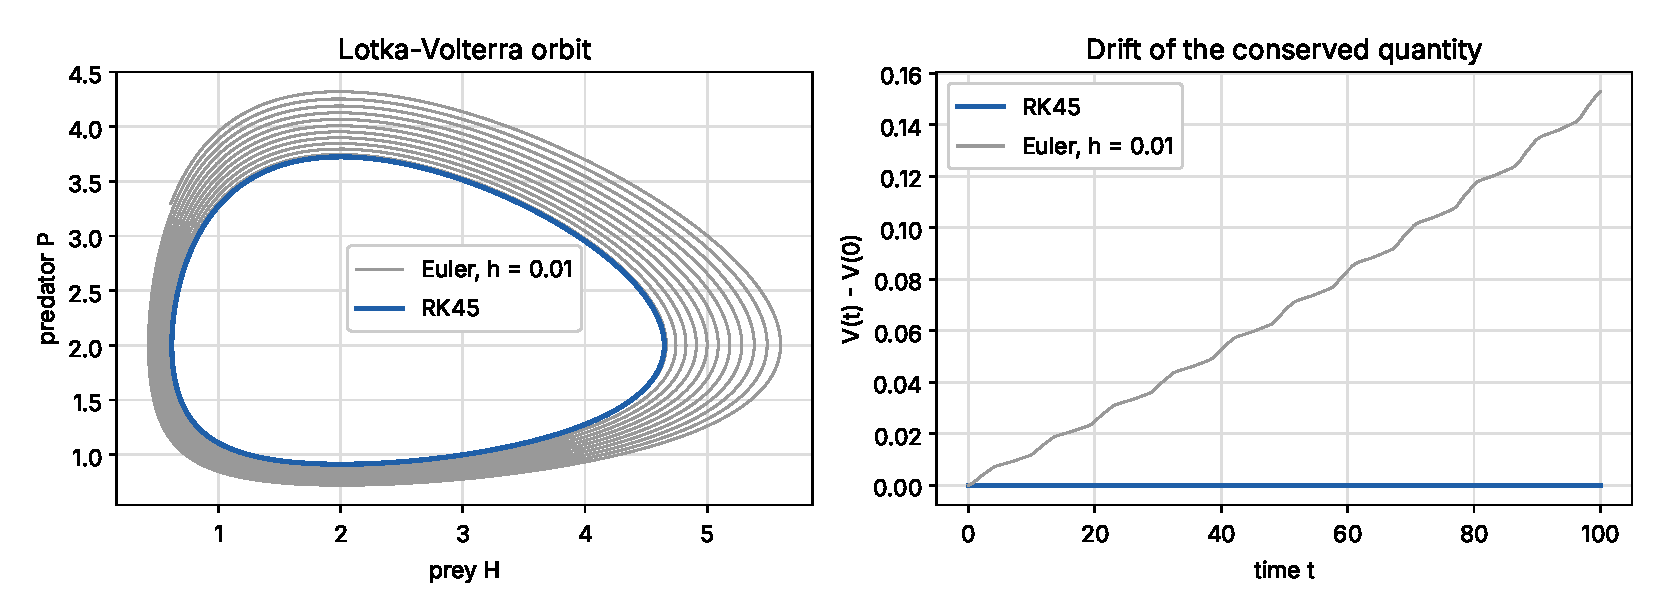
\includegraphics[width=0.9\linewidth]{rishi_solver_validation}
  \caption{Solver check on Lotka--Volterra. RK45 preserves the conserved quantity $V$ and
  closes the orbit; Euler ($h=0.01$) drifts and spirals outward. Only an accurate solver can
  distinguish a genuine limit cycle from a numerical artefact.}
  \label{fig:rishi_solver}
\end{figure}

\subsection{Reproduction of the analytic regimes}

Table~\ref{tab:rishi_regimes} reproduces each validation target of Section~\ref{sec:joel}
(3000-year burn-in throughout). Regime~D lies exactly on $K_H$: the residual oscillation there is
a slowly decaying transient (decay is only algebraic at a weak focus), not a cycle.

\begin{table}[htbp]
  \centering
  \caption{Simulated long-run behaviour for the regimes of Section~\ref{sec:joel}. Ranges are
  over 400 years after the burn-in; period and lynx lag are in years.}
  \label{tab:rishi_regimes}
  \begin{tabular}{clccccc}
    \toprule
    & $K$ & Eigenvalues & $H$ range & $P$ range & Period & Lag \\
    \midrule
    A & 25  & $-1.5,\ -0.073$ ($E_1$) & $25.0$         & $0$              & -- & -- \\
    B & 60  & $-0.188\pm0.515i$ & $30.0$         & $11.25$          & -- & -- \\
    C & 85  & $-0.022\pm0.623i$ & $30.0$         & $14.56$          & -- & -- \\
    D & 90  & $\pm0.632i$       & $[28.5,31.6]$  & $[14.51,15.49]$  & 9.94  & 2.50 \\
    E & 95  & $+0.020\pm0.640i$ & $[15.8,50.9]$  & $[9.81,20.75]$   & 10.25 & 2.81 \\
    F & 150 & $+0.150\pm0.676i$ & $[1.1,134.3]$  & $[1.69,41.16]$   & 13.91 & 4.52 \\
    \bottomrule
  \end{tabular}
\end{table}

Figure~\ref{fig:rishi_regimes} shows four of these regimes. Below the threshold (B, C) the
predator nullcline meets the prey hump to the right of its peak and trajectories spiral into
$E^*$; at $K=85$ the trace is only $-0.044$, so the decay takes centuries. Above the threshold
(E, F) the intersection lies left of the peak, $E^*$ repels, and the orbit settles onto a
sustained cycle that circulates counter-clockwise, with lynx peaks lagging hare peaks.

\begin{figure}[htbp]
  \centering
  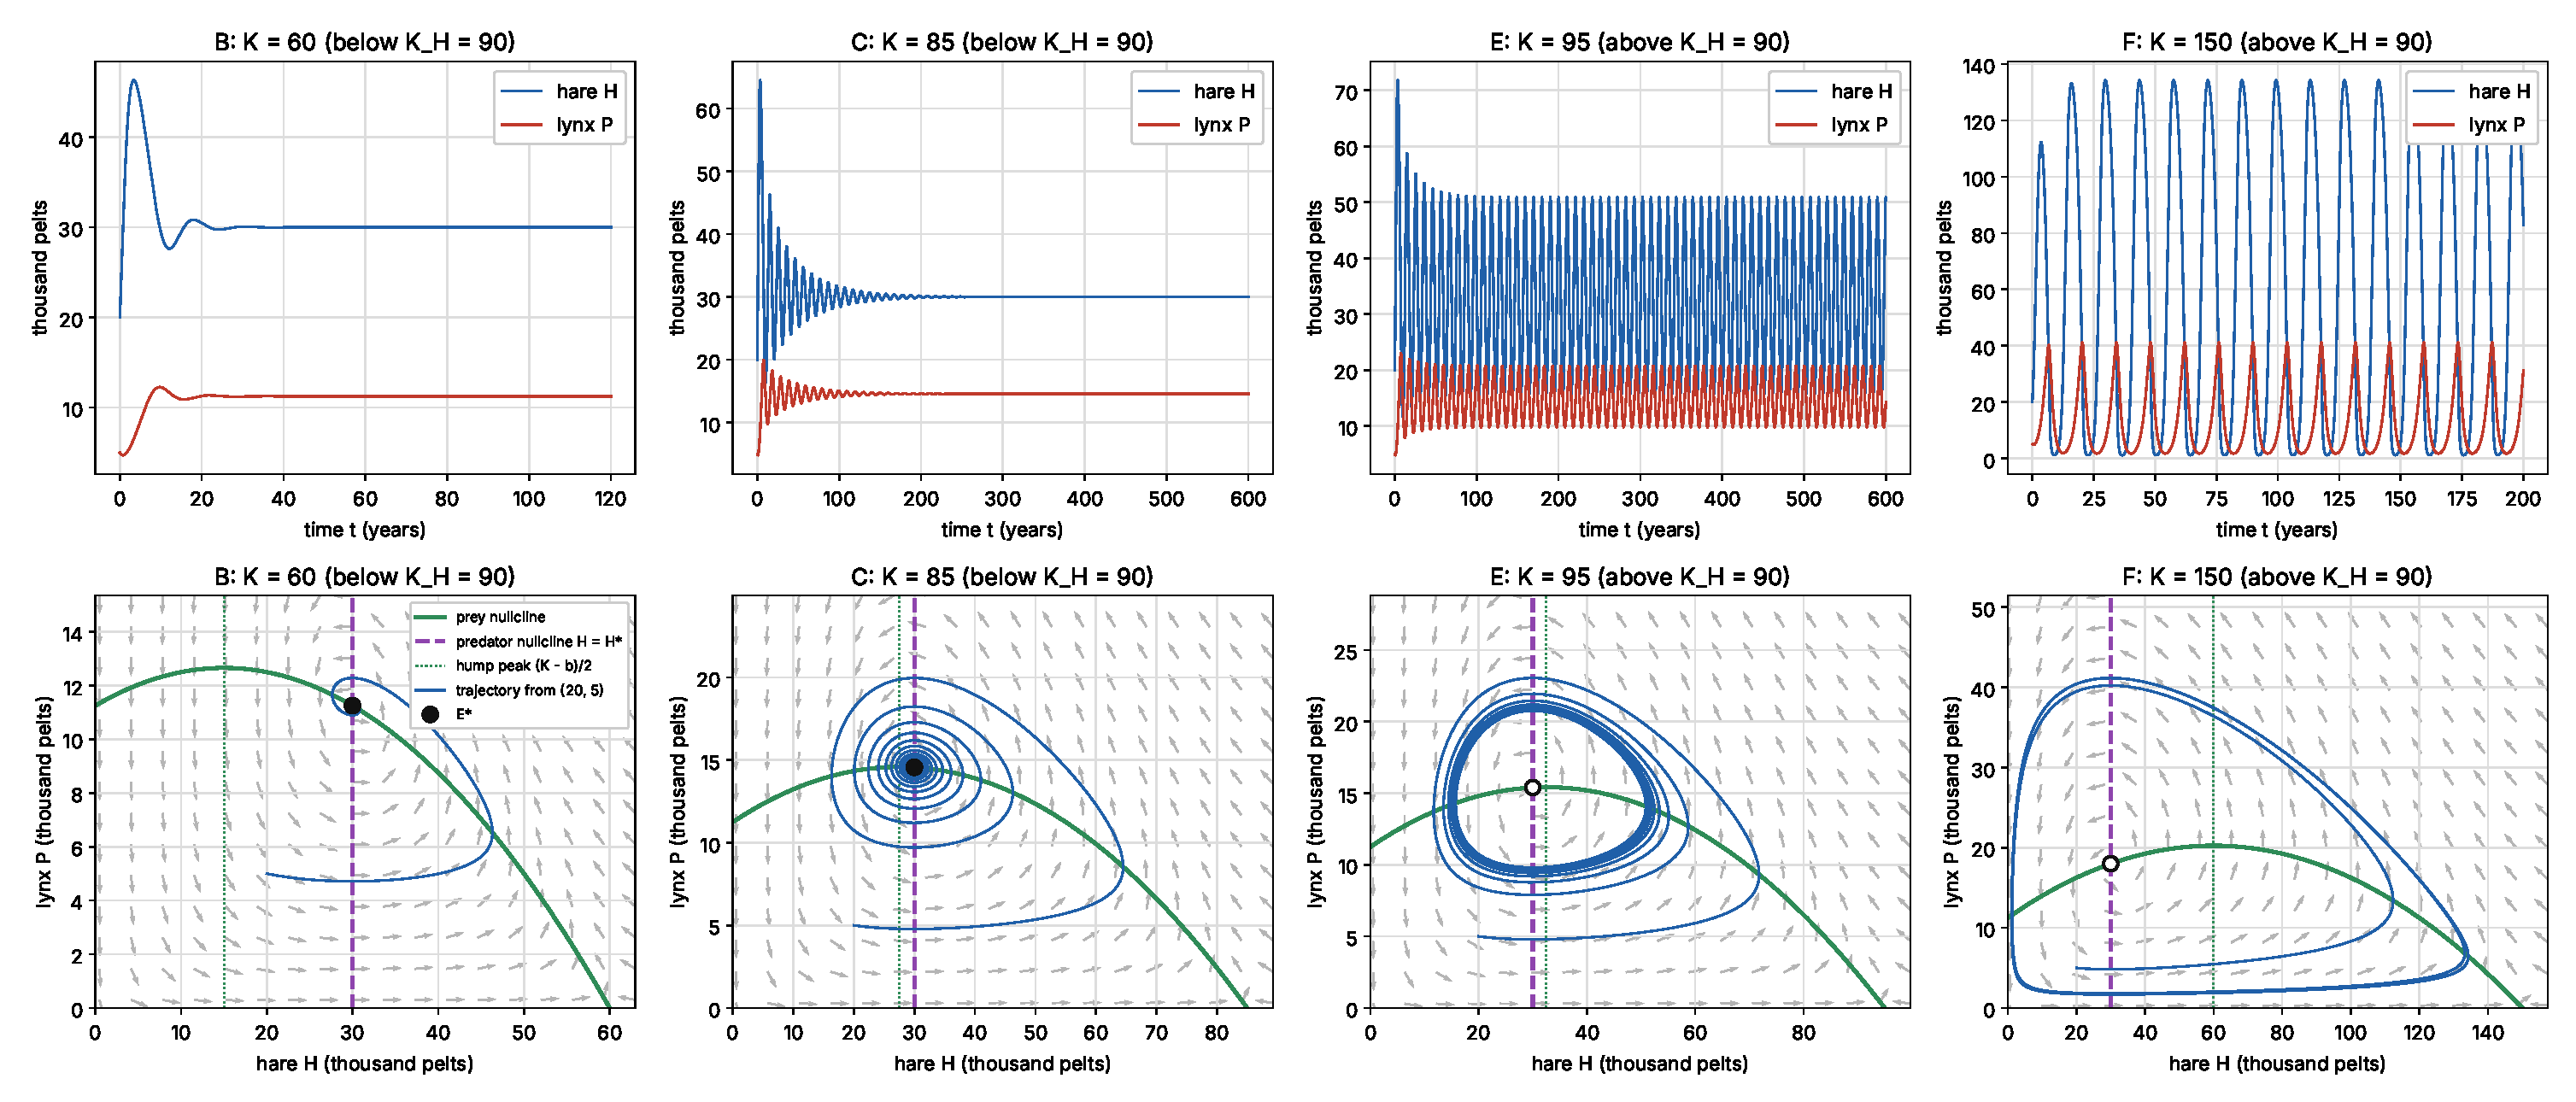
\includegraphics[width=\linewidth]{rishi_regimes}
  \caption{Time series (top) and phase portraits (bottom) from $(20,5)$ for $K=60,85$ (below
  $K_H=90$) and $K=95,150$ (above). Green: prey nullcline; dashed purple: predator nullcline
  $H=H^*$; dotted: hump peak $(K-b)/2$. Filled/open circle: stable/unstable $E^*$. Oscillations
  decay below $K_H$ and persist above it.}
  \label{fig:rishi_regimes}
\end{figure}

\subsection{The limit cycle attracts}

For Lotka--Volterra every initial condition lies on its own closed orbit. At $K=150$ we start one
trajectory beside the unstable equilibrium and one far outside the cycle
(Figure~\ref{fig:rishi_cycle}). The first spirals outward, the second inward, and their successive
hare maxima converge to the same value, $134.277$. The cycle is therefore orbitally stable,
in agreement with the uniqueness result cited in Section~\ref{sec:joel}~\cite{cheng1981}.

\begin{figure}[htbp]
  \centering
  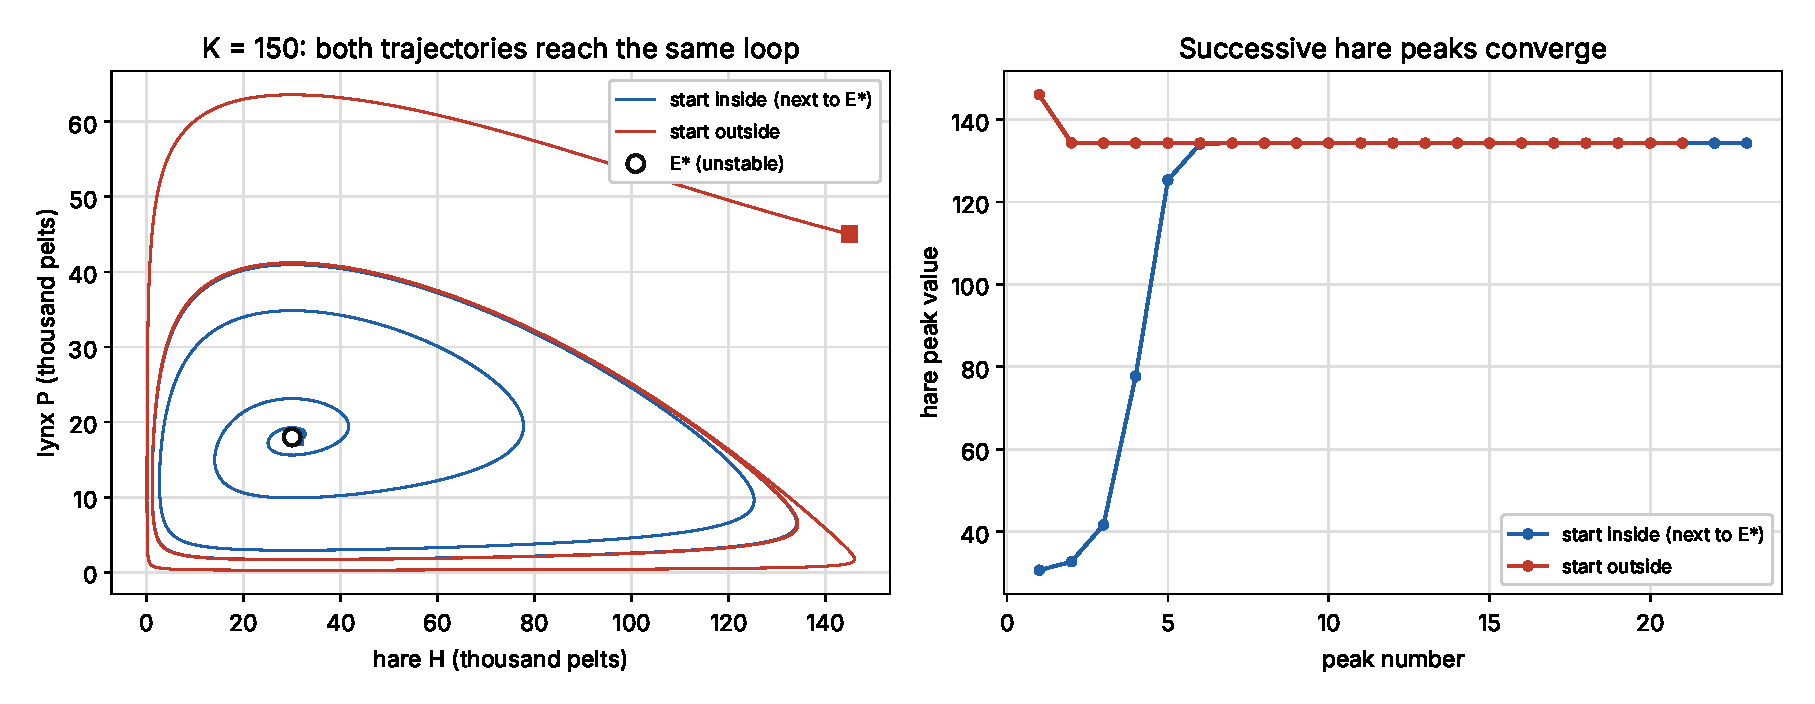
\includegraphics[width=0.9\linewidth]{rishi_limit_cycle}
  \caption{At $K=150$, trajectories started inside and outside the cycle converge onto the same
  closed orbit (left); their successive hare maxima approach a common value (right).}
  \label{fig:rishi_cycle}
\end{figure}

\subsection{Bifurcation in $K$}

Root-finding on the numerically evaluated trace of $J(E^*)$ places the sign change at
$K=90.0000000000$, in agreement with $K_H=b+2H^*$ and Figure~\ref{fig:trace-det}; there the
eigenvalues are $\pm0.632i=\pm i\omega_0$, and they become complex (node to focus) at $K\approx42.6$.

The numerical bifurcation diagram (Figure~\ref{fig:rishi_bif}) records the post-transient maximum
and minimum for 113 values of $K$ between 32 and 200. For $K<89$ the two coincide (largest
spread $5\times10^{-5}$): the solution settles on $E^*$. At $K_H$ the branches separate continuously
from the equilibrium and the cycle grows with $K$. Just above the threshold its half-amplitude
follows $A\approx7.8\sqrt{K-K_H}$, with fitted log--log slope $0.507$ for $0.5\le K-K_H\le8$
(Figure~\ref{fig:rishi_amp}), and the period approaches $T_0=9.93$ years ($9.97$ years at
$K-K_H=0.5$). This square-root growth from zero amplitude is the signature of a supercritical
Hopf bifurcation, consistent with the negative first Lyapunov coefficient of
Section~\ref{sec:joel}. As $K$ increases further the cycle minima approach zero: at $K=200$ the
hare minimum is $0.12$ thousand pelts, the paradox of enrichment~\cite{rosenzweig1971}.

\begin{figure}[htbp]
  \centering
  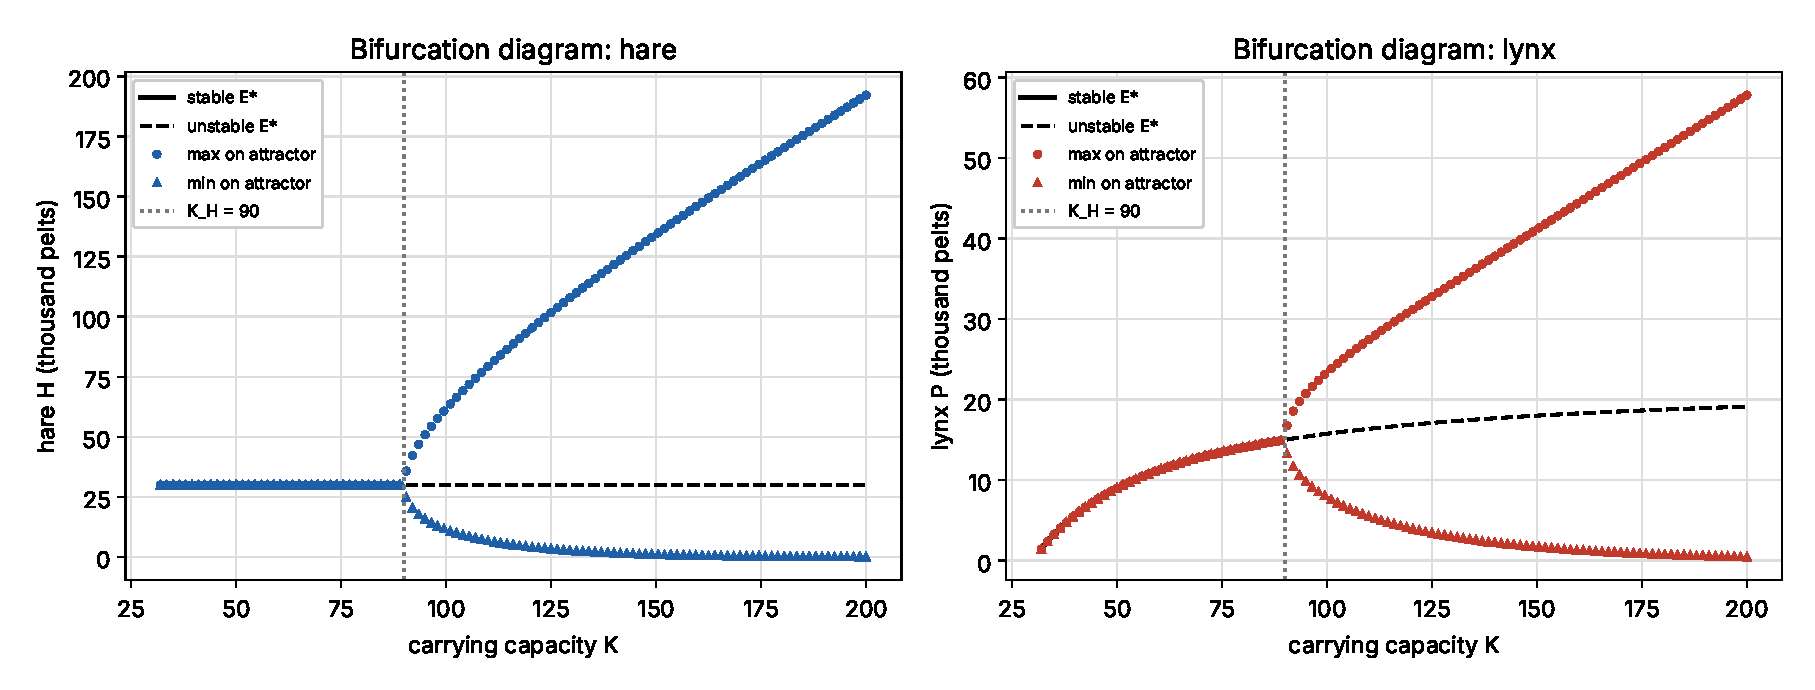
\includegraphics[width=0.9\linewidth]{rishi_bifurcation}
  \caption{Numerical bifurcation diagram: maximum and minimum of $H$ (left) and $P$ (right) after
  the burn-in, against $K$. Solid/dashed black: stable/unstable $E^*$. A cycle is born at
  $K_H=90$ with zero amplitude and its minima approach zero as $K$ grows.}
  \label{fig:rishi_bif}
\end{figure}

\begin{figure}[htbp]
  \centering
  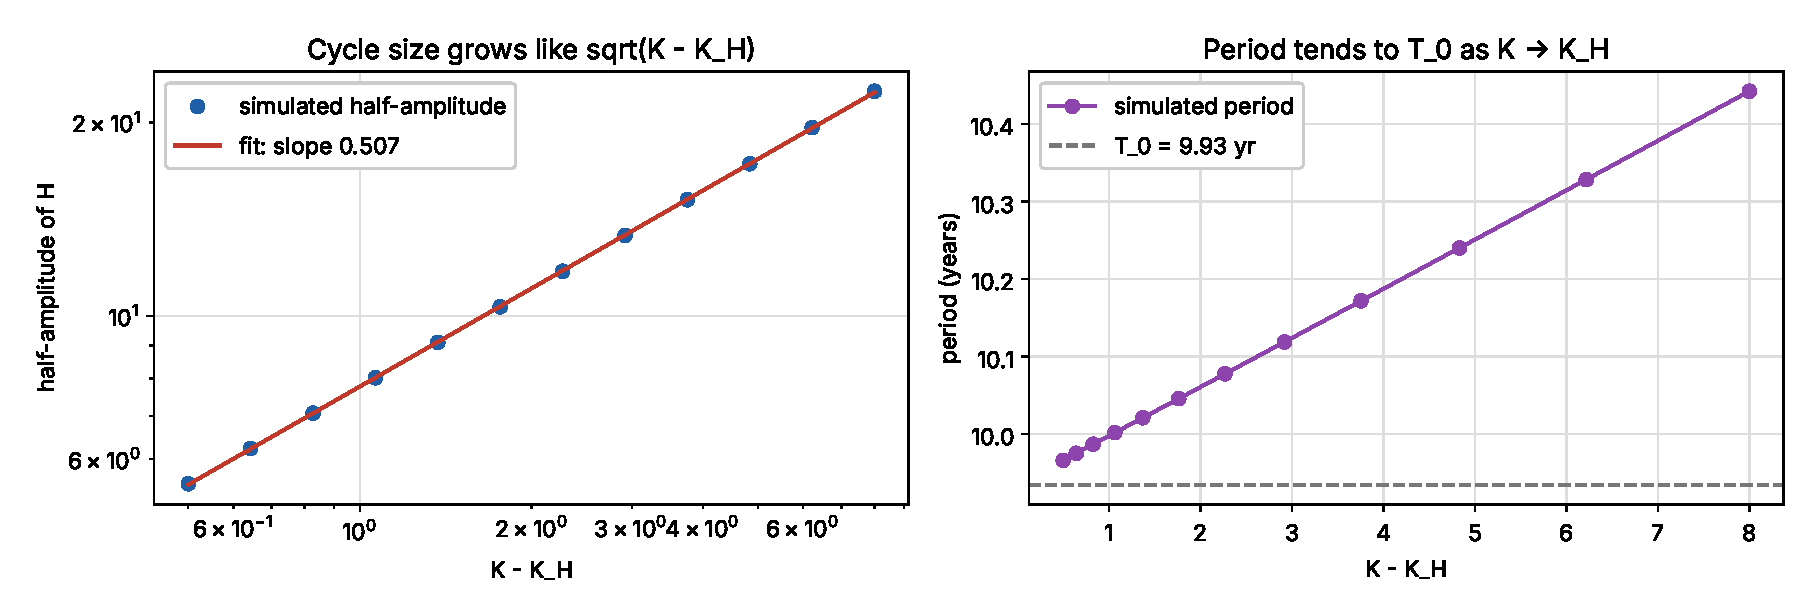
\includegraphics[width=0.9\linewidth]{rishi_amplitude_period}
  \caption{Left: half-amplitude of $H$ against $K-K_H$ on log--log axes, with slope $0.507$
  (supercritical prediction $1/2$). Right: cycle period, tending to $T_0=2\pi/\omega_0$.}
  \label{fig:rishi_amp}
\end{figure}

\subsection{Scope}

These simulations use illustrative, unfitted parameters and provide numerical evidence for one
parameter set, not proofs. Near $K_H$ the results depend on the burn-in length, which is why it
is lengthened there. Whether the historical hare--lynx series lies above or below the threshold
depends on $\sigma=K/K_H$ at the fitted parameters and is addressed in the fitting sections.
\clearpage
\section{Historical inverse PINN study}
This is Yash's contribution, using the historical pelt series supplied by Advay. It
extends the separately preserved synthetic recovery experiment; it is not a complete
combined group report. The Stan compilation contains annual Hudson's Bay Company
hare and lynx pelt returns \cite{carpenter2018}. We train on 1900--1915 (16 pairs) and
evaluate once on frozen forecasts for 1916--1920 (five pairs). Counts are thousands of
pelts, treated as abundance indices rather than censuses. Annual totals are approximated
as point samples. No observation scale factor is fitted. Alternative source compilations
disagree; all results here are conditional on the Stan series.

\subsection{Model and protocol}
With $t=\mathrm{Year}-1900$, the shared dimensional model is
\begin{align*}
\dot H&=rH(1-H/K)-aHP/(b+H), & \dot P&=eaHP/(b+H)-mP.
\end{align*}
All six positive coefficients are inferred. Bounds below are exploratory numerical
choices, not measured biological ranges. No coexistence constraint is imposed and $e$
is not constrained below one because these are effective coefficients in pelt units.
The starting vector is $(r,K,a,b,e,m)=(0.8,150,2,30,0.6,0.6)$. Yash chose this protocol
with assistance; agreement by the other members is not claimed. The local least-squares
benchmark uses the identical config, data split, scaling and solver.
\begin{center}\begin{tabular}{lrr}\toprule
Coefficient & Bounds & Selected primary estimate\\\midrule
$r$ & 0.05--3 & 0.60546 \\
$K$ & 20--500 & 497.6 \\
$a$ & 0.05--10 & 9.2605 \\
$b$ & 0.5--300 & 299.98 \\
$e$ & 0.02--5 & 1.0966 \\
$m$ & 0.05--3 & 0.99388 \\
\bottomrule\end{tabular}\end{center}

\subsection{Network, loss and optimization}
The inverse PINN \cite{raissi2019} uses three hidden layers of 48 tanh units, float64,
softplus-positive normalized outputs, and sigmoid-bounded coefficients. Species scales
are training maxima $(s_H,s_P)=(77.4,59.4)$; network time is $2t/15-1$.
For $u_\theta=(H_\theta/s_H,P_\theta/s_P)$, automatic differentiation evaluates
$R_\theta=\partial_tu_\theta-f(u_\theta\odot s;p)/s$. The loss is
\[
L=\operatorname{mean}(u_\theta-y/s)^2+
10\operatorname{mean}R_\theta^2+
10\operatorname{mean}(u_\theta(0)-y_0/s)^2.
\]
The initial observation is $y_0=(30,4)$. There are 161 collocation times in $[0,15]$.
Optimization uses 500 data/IC warmup steps, up to 5000 joint Adam steps at learning rate
0.002 (gradient norm clipped at 10), then up to 600 L-BFGS iterations with strong-Wolfe
line search. Training loss is logged every 100 Adam steps; plateau stopping uses
15 checks and minimum improvement $10^{-8}$. The best recorded weighted training
objective determines the saved state. Seeds are 17, 29 and 43, with one CPU thread and
deterministic Torch operations. Each variant selects its own lowest-loss seed; objectives
from different observation models are not used to select the primary analysis.
\begin{figure}[htbp]\centering
\ReportGraphEPS[width=\linewidth]{yash_historical_fit.eps}
\caption{Training observations, learned network and re-integrated ODE. A small local
physics residual does not guarantee identical long-horizon ODE and network trajectories.}
\end{figure}

\subsection{Frozen forecasts and matched benchmark}
The selected primary seed is 17. Forecasts use the learned coefficients in the shared
RK45 solver with rtol $10^{-8}$, atol $10^{-10}$ and maximum step 0.1 year. Integration
starts from $(30,4)$ in 1900 and proceeds through 1920, with no restart from a test state.
The neural network is never extrapolated for forecasting. Its starting-state discrepancy
is $(0.10060,-0.00723)$ thousand pelts; the ODE still starts at the exact observation.
The primary ODE training normalized MSE is 0.00981. The matched primary least-squares
fit uses six starts (RNG seed 91), bounded \texttt{least\_squares}, up to 500 function
evaluations and ftol=xtol=gtol=$10^{-10}$. Each start and its convergence status is retained.
This is an independent benchmark computed for this contribution; Advay's own historical
baseline is not represented as completed. PINN and least squares differ in soft versus
exact IC enforcement and in the PINN's added physics penalty.
\begin{figure}[htbp]\centering
\ReportGraphEPS[width=\linewidth]{yash_historical_forecast.eps}
\caption{Frozen forecasts. Thin pale lines are the three primary PINN seeds, not confidence
bands. Shading marks held-out years; observations were used for scoring only after all
forecast and seed choices were frozen.}
\end{figure}
\begin{center}\small\begin{tabular}{lrrrr}\toprule
& \multicolumn{2}{c}{RMSE} & \multicolumn{2}{c}{MAE}\\
Method & Hare & Lynx & Hare & Lynx\\\midrule
PINN fitted IC & 3.687 & 4.697 & 3.057 & 4.530 \\
PINN log errors & 18.351 & 10.026 & 14.289 & 8.972 \\
PINN primary & 2.847 & 4.317 & 2.590 & 4.046 \\
PINN wider bounds & 2.976 & 4.053 & 2.721 & 3.779 \\
PINN physics 100 & 4.519 & 3.978 & 4.107 & 3.496 \\
LS primary & 3.072 & 3.043 & 2.586 & 2.559 \\
LS log errors & 6.874 & 1.596 & 6.626 & 1.381 \\
LS fitted IC & 2.246 & 3.236 & 2.083 & 2.713 \\
\bottomrule\end{tabular}\end{center}
All scores are thousands of pelts on the same five held-out years. The primary PINN has
slightly lower hare RMSE than primary least squares, but higher lynx RMSE. Hare MAE is
essentially tied. These results do not establish an overall PINN advantage.
\begin{figure}[htbp]\centering
\ReportGraphEPS[width=0.95\linewidth]{yash_historical_loss.eps}
\caption{Selected primary training loss components. L-BFGS abscissae count closure
evaluations after Adam; they are not directly comparable computational steps.}
\end{figure}

\subsection{Sensitivity and practical identifiability}
All sensitivities were specified before any test scoring and are reported regardless
of outcome. The main three seeds were repeated with log observation residuals, and
separately with trainable initial states in $[0.5,1.5]$ times the 1900 observations. The
first data point stays in the data loss. The fitted-IC PINN's ODE starts at approximately
$(34.7477,3.7841)$; the network and ODE initial states are separately recorded. The benchmark
repeats both observation/IC sensitivities with six starts each. Log residuals worsen hare
forecast error for both methods, especially the PINN. None of these scores changes the
predeclared primary choice.

To check arbitrary box limits, each lower bound was halved and each upper bound doubled,
and the main PINN was repeated for all three seeds. A further seed-17 run increased physics
weight from 10 to 100. In total there are 13 PINN runs and 18 least-squares starts.
The wider-box fits move $K$ from about 498 to about 986 and $b$ from about 300 to about 600,
close to the expanded limits; $a$ also shifts substantially. Similar results across seeds
therefore do not demonstrate uniquely recovered biological parameters. The wider-box
forecast changes are smaller than these coefficient shifts.
\begin{figure}[htbp]\centering
\ReportGraphEPS[width=\linewidth]{yash_historical_bounds.eps}
\caption{Primary versus wider-box parameter estimates over three seeds. Several effective
coefficients track the numerical bounds; narrow seed spread is not parameter certainty.}
\end{figure}
\begin{figure}[htbp]\centering
\ReportGraphEPS[width=\linewidth]{yash_historical_sensitivity.eps}
\caption{All selected PINN variants. The log-error fit shows appreciable model/ODE forecast
sensitivity. Variants were retained rather than chosen using held-out errors.}
\end{figure}

\clearpage
The local trajectory sensitivity matrix uses central differences with respect to log
parameters (step $10^{-4}$), normalized using the declared observation loss. Its selected
primary condition number is approximately 317.5. This is a local diagnostic, not
a proof of structural identifiability or a confidence interval. For feasible coexistence,
$H^*=mb/(ea-m)$, $K_H=b+2H^*$ and $\sigma=K/K_H$; the selected primary fit gives
$\sigma=1.363$. This fitted ODE lies on the cycling side of Joel's threshold, conditional
on the model and protocol. It does not prove that the historical ecological system has
a stable limit cycle. All seeds' values and feasibility flags are exported to the team.

\subsection{Reproducibility and limitations}
\path{configs/historical.json} records every primary choice; the two sensitivity
configs record the expanded box and physics weight. Run manifests hash sources, config,
training data, forecasts and diagnostics. A forecast-freeze record is written before the
test observations are read. \path{scripts/run_historical_pinn.py} accepts only the
training table; \path{scripts/score_historical.py} handles final scoring. Existing
synthetic recovery results are preserved as a separate controlled validation.

Six effective coefficients are fitted from roughly two noisy cycles; boundary hits,
source disagreement, annual season totals, unknown catchability and the small test window
limit interpretation. PINN physics is a soft constraint, and the log-loss variant exposes
an appreciable network/ODE discrepancy. Seed spread is optimization sensitivity only.
Forecast skill on five points cannot establish general superiority, causal mechanisms
or absolute animal populations. This report and notebook concern Yash's component;
the final group report and submission still require integration.

\paragraph{PINN optimization gap.}
Advay independently evaluated the training observation objective on the frozen
PINN-derived ODE trajectories. Their costs are 1.859, 3.396 and 1.866 times the
least-squares minima for main, log-error and fitted-initial-state variants. These
are observation costs, not the PINN's weighted neural training loss. The PINN optimizes
a soft-physics network objective, and reintegration can accumulate phase error; it
does not attain the least-squares optimum here. These diagnostics motivate the
reported limitations and do not trigger post-test retuning.
\clearpage% Advay: data, least-squares baseline, held-out evaluation and limitations.
% Drop-in file:  % Advay: data, least-squares baseline, held-out evaluation and limitations.
% Drop-in file:  % Advay: data, least-squares baseline, held-out evaluation and limitations.
% Drop-in file:  \input{advay_data_validation_section}   (standalone build: advay_main.tex)
% Figures: graphs/advay_*.{eps,pdf}; table: tables/advay_heldout_metrics.tex.
\section{Data, Least-Squares Baseline and Validation}\label{sec:advay}

This section states what the historical observations are, how they were prepared, how the
model was fitted to them by nonlinear least squares, and how well the fitted model forecasts
years it never saw. Every analysis choice that could be influenced by the held-out years was
written down and committed to the project repository before those years were opened.

\subsection{Data source and meaning}\label{sec:advay-data}

We use annual counts of snowshoe hare and Canadian lynx pelts traded by the Hudson's Bay
Company, 1900--1920, in thousands of pelts, as distributed with the Stan case study
\cite{carpenter2018}. Carpenter traces the numbers through Howard's lecture notes
\cite{howard2009} to a biology textbook; the original source is the Company's fur returns,
discussed by Hewitt \cite{hewitt1921}. The values are used unchanged
(\texttt{data/historical/pelts\_1900\_1920.csv}); the file's provenance, checksums and every
transformation (removing comment lines, reordering columns) are recorded alongside it.

These are \emph{trade counts}, not censuses. Trapping effort, fur prices, the number of
reporting posts and animal behaviour all affect them; Hewitt notes that hungry lynx are
easier to trap when hares are scarce. A second widely used compilation, the tsibbledata
\texttt{pelt} series \cite{tsibbledata_pelt}, differs noticeably over the same years
(Figure~\ref{fig:advay-sources}): the correlation between the two is 0.81 for lynx but only
0.32 for hare, and individual hare values differ by more than our forecast errors. We use
the Stan series because the project protocol names it, and treat the disagreement as a source
of uncertainty that no model in this report can remove.

\begin{figure}[ht]
\centering
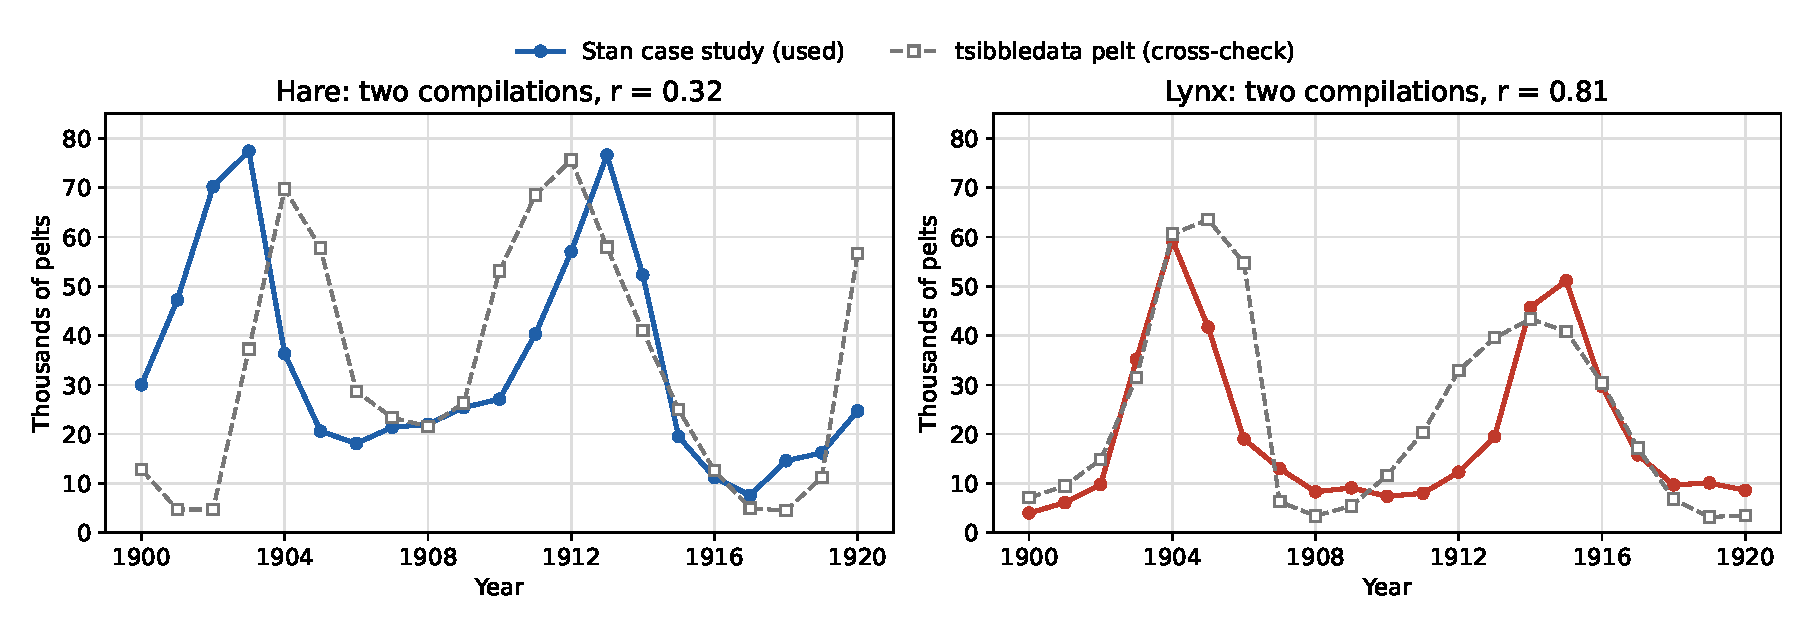
\includegraphics[width=\textwidth]{advay_source_comparison}
\caption{The Stan case-study series used here (solid) and the tsibbledata \texttt{pelt}
compilation (dashed) for 1900--1920. Both show two cycles, but yearly values differ,
especially for hare.}\label{fig:advay-sources}
\end{figure}

\paragraph{Observation model.} Following the agreed convention (assumption O1), pelt counts
are taken to be proportional to animal numbers with unknown constant factors, and the model
states are defined directly in pelt units:
\[
Y_{H,i}=H(t_i)+\varepsilon_{H,i},\qquad Y_{P,i}=P(t_i)+\varepsilon_{P,i},\qquad t_i=\mathrm{Year}_i-1900,
\]
with each annual total treated as a sample of the state at $t_i$. No observation scale factor
is fitted. Under O1, $r$, $m$ and the dimensionless groups of the model section are unchanged
by the unknown factors; $K$, $b$, $a$ and $e$ are \emph{effective} coefficients in pelt
units and are not interpreted as absolute biological quantities.

\subsection{Preparation and exploratory checks}\label{sec:advay-checks}

The 21 rows are consecutive, with no missing values, no zeros and no duplicates. The data
were split once into a training file (1900--1915, 16 rows) and a test file (1916--1920,
5 rows), with checksums recorded; all fitting code reads only the training file. Every
statistic below uses the training years only.

\begin{itemize}
\item \textbf{Cycles and lag.} Hare peaks in 1903 and 1913 (a ten-year spacing); lynx peaks
in 1904 and at the 1915 boundary. The correlation of $H(t)$ with $P(t+k)$ is largest at
$k=2$ years ($r=0.94$; $0.76$ at $k=1$). In the hare--lynx plane the data trace
counter-clockwise loops, as predator--prey models predict (Figure~\ref{fig:advay-raw}).
\item \textbf{Outliers.} None: robust $z$-scores of year-to-year log growth stay below 3
(largest 2.94, the 1903--1904 hare crash).
\item \textbf{Scale.} Training ranges are 18.1--77.4 (hare) and 4.0--59.4 (lynx). Hare counts
are about twice lynx counts, so residuals are divided by each species' training maximum
$(s_H,s_P)=(77.4,59.4)$ to weight the species equally. No log transform is used in the main
analysis; a log-residual fit is a declared sensitivity check.
\item \textbf{Split position.} Training ends exactly at the 1915 lynx peak, so the test years
are the following crash and the start of recovery: a turning point the fit never sees in
that cycle.
\end{itemize}

\begin{figure}[ht]
\centering
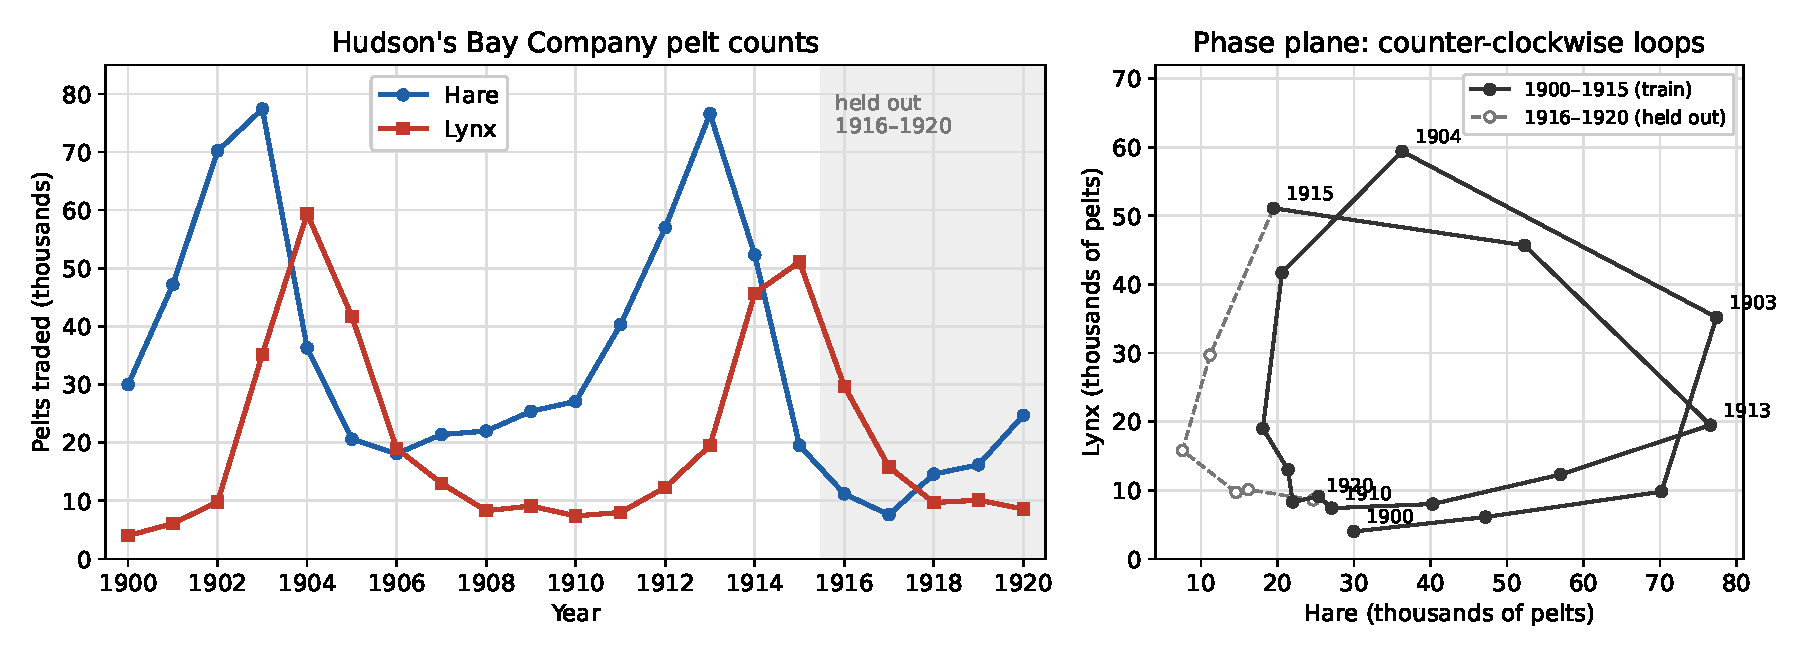
\includegraphics[width=\textwidth]{advay_raw_series}
\caption{Left: annual pelt counts, 1900--1920; the shaded band is held out. Right: the same
data in the hare--lynx plane (training solid, held-out dashed).}\label{fig:advay-raw}
\end{figure}

\subsection{Least-squares baseline}\label{sec:advay-ls}

\paragraph{Problem.} With $\theta=(r,K,a,b,e,m)$ and the shared RK45 solver (relative
tolerance $10^{-8}$, absolute $10^{-10}$, maximum step $0.1$ years), let $\hat H(t;\theta)$,
$\hat P(t;\theta)$ solve the model from the observed 1900 state $(30.0,4.0)$. The main
estimate minimises
\[
C(\theta)=\tfrac12\sum_{i=1900}^{1915}\Big[\big(\tfrac{\hat H(t_i;\theta)-Y_{H,i}}{s_H}\big)^2+
\big(\tfrac{\hat P(t_i;\theta)-Y_{P,i}}{s_P}\big)^2\Big]
\]
over the shared box bounds $r,m\in[0.05,3]$, $K\in[20,500]$, $a\in[0.05,10]$,
$b\in[0.5,300]$, $e\in[0.02,5]$. Two declared sensitivity variants change one assumption
each: \emph{log errors} replaces the scaled residuals by $\log\hat Y-\log Y$, and
\emph{fitted 1900 state} adds $(H_0,P_0)$ as unknowns within $[0.5,1.5]$ times the observed
values.

\paragraph{Method.} The bounded trust-region reflective algorithm (SciPy
\texttt{least\_squares}) is run in log-parameter space $x=\log\theta$, because the bounds
span up to a 600-fold range. Finite-difference steps of $10^{-4}$ in $x$ stay well above the
solver tolerance. The objective is multimodal, so each variant uses 80 starts: the shared
initial guess, 39 Latin-hypercube points uniform in $\log\theta$ and 39 uniform in $\theta$.
The fit with the lowest training cost is selected.

\paragraph{Protocol record.} The settings were committed before the first run. That run
(40 log-space starts) missed the best \emph{fitted 1900 state} fit, which an independent
benchmark had found at training cost $0.063$ against our $0.70$; evaluating our objective at
the benchmark's parameters gave $0.063$, so the code agreed and the start design was at
fault (the optimum sits near the upper bounds, which log-uniform starts rarely visit). The
uniform-scale starts were added as a declared amendment, judged on training cost alone and
before any test score of the baseline was computed. Both runs are kept.

\begin{table}[ht]
\centering
\begin{tabular}{lrrrrrrrl}
\toprule
Variant & $C$ & $r$ & $K$ & $a$ & $b$ & $e$ & $m$ & $\sigma=K/K_H$\\
\midrule
Main & 0.0845 & 0.647 & 382 & 10.0$^*$ & 300$^*$ & 0.967 & 0.857 & 1.07 (cycle)\\
Log errors & 0.903 & 0.520 & 197 & 7.17 & 300$^*$ & 1.80 & 1.15 & 0.55 (damped)\\
Fitted 1900 state & 0.0634 & 0.520 & 362 & 8.15 & 300$^*$ & 1.32 & 1.05 & 0.99 (damped)\\
\bottomrule
\end{tabular}
\caption{Least-squares estimates. $^*$ at the upper bound. Units: $r,m$ per year; $K,b$
thousands of hare pelts; $a,e$ effective pelt-unit coefficients. The fitted 1900 state in the
last variant is $(37.1,3.64)$.}\label{tab:advay-ls}
\end{table}

\paragraph{Results.} Table~\ref{tab:advay-ls} and Figure~\ref{fig:advay-fit} give the selected
fits. Three findings matter for interpretation.
\begin{enumerate}
\item \emph{The optimum is computationally well defined.} In every variant all starts within
1\% of the best cost (18, 42 and 16 of 80) found the same parameters to four significant
figures, and a separately written least-squares code by another team member reaches the same
optimum (training costs within $2\times10^{-7}$, forecasts within 0.002 thousand pelts).
\item \emph{The saturation of predation is not identified.} $b$ sits on its upper bound in
every variant. With $b$ about four times the largest hare count, $aH/(b+H)\approx(a/b)H$ over
the data: predation is nearly linear in hare abundance. In the linearised fit the
correlation between $\log a$ and $\log b$ is 0.998 and the approximate standard errors of
$\log K$, $\log a$, $\log b$ exceed 1 (a factor of three or more), whereas $r$, $e$, $m$ are
determined to about 10--40\%. Only the ratio $a/b\approx0.024$--$0.033$ is well determined.
Because the optimum lies on the boundary, its location depends on the chosen box.
\item \emph{Limit cycle or damped oscillation is not decided.} Using the Hopf threshold
$K_H=b(ea+m)/(ea-m)$ from the stability analysis, $\sigma$ is 1.07 for the main fit (just past the threshold),
0.99 with a fitted 1900 state (just below) and 0.55 with log errors. All three reproduce the
observed timing equally well (hare peaks fitted at 1902.5--1902.8 and 1912.6--1913.0, lynx
1.6 years later, period about ten years). Two cycles of data cannot distinguish a stable
limit cycle from a slowly damped oscillation (Figure~\ref{fig:advay-sigma}).
\end{enumerate}

\begin{figure}[ht]
\centering
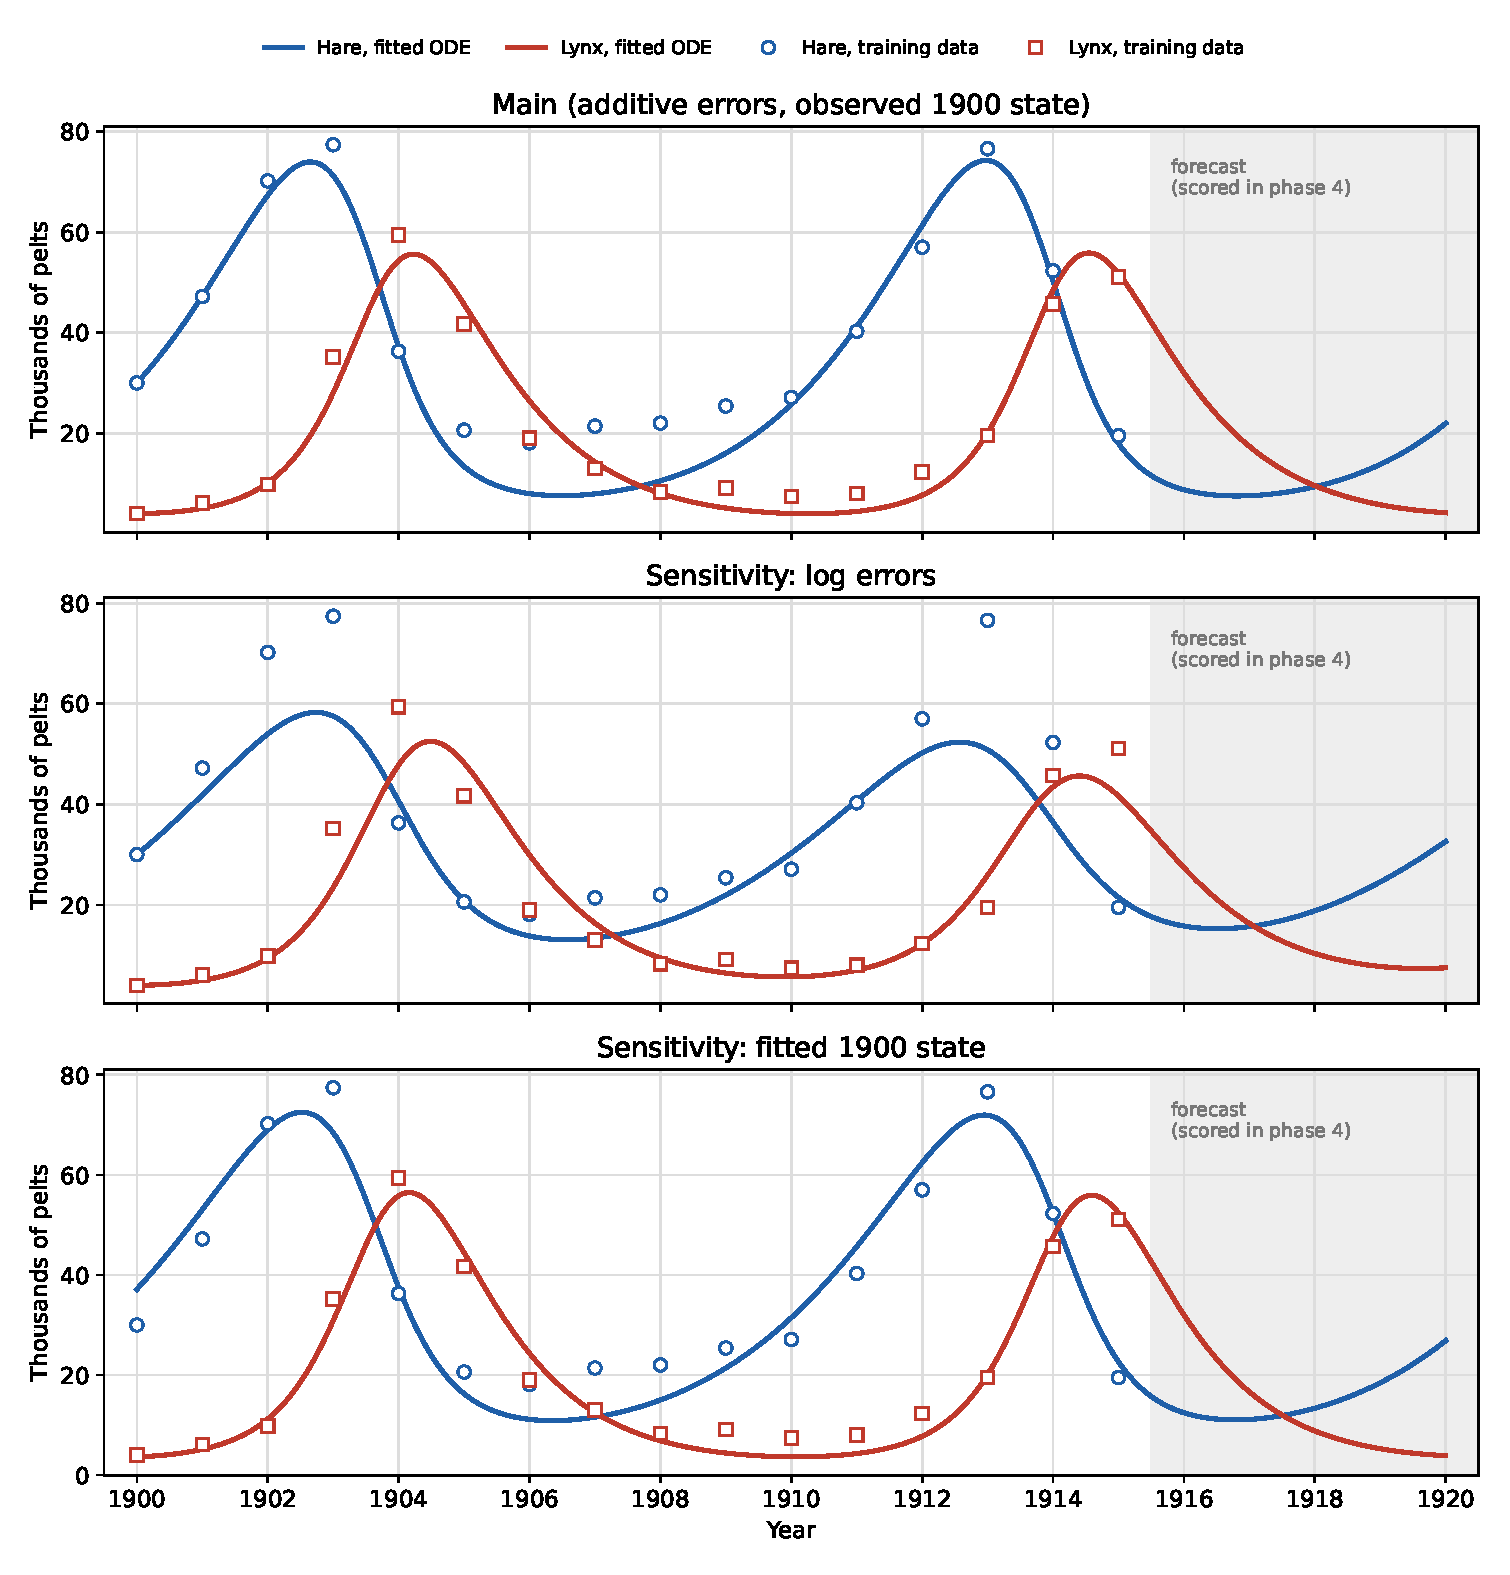
\includegraphics[width=0.9\textwidth]{advay_baseline_fit}
\caption{Least-squares fits to the 1900--1915 pelt counts (markers) and their continuation
through 1920 (shaded, held out) for the main analysis and both sensitivity variants.}
\label{fig:advay-fit}
\end{figure}

\begin{figure}[ht]
\centering
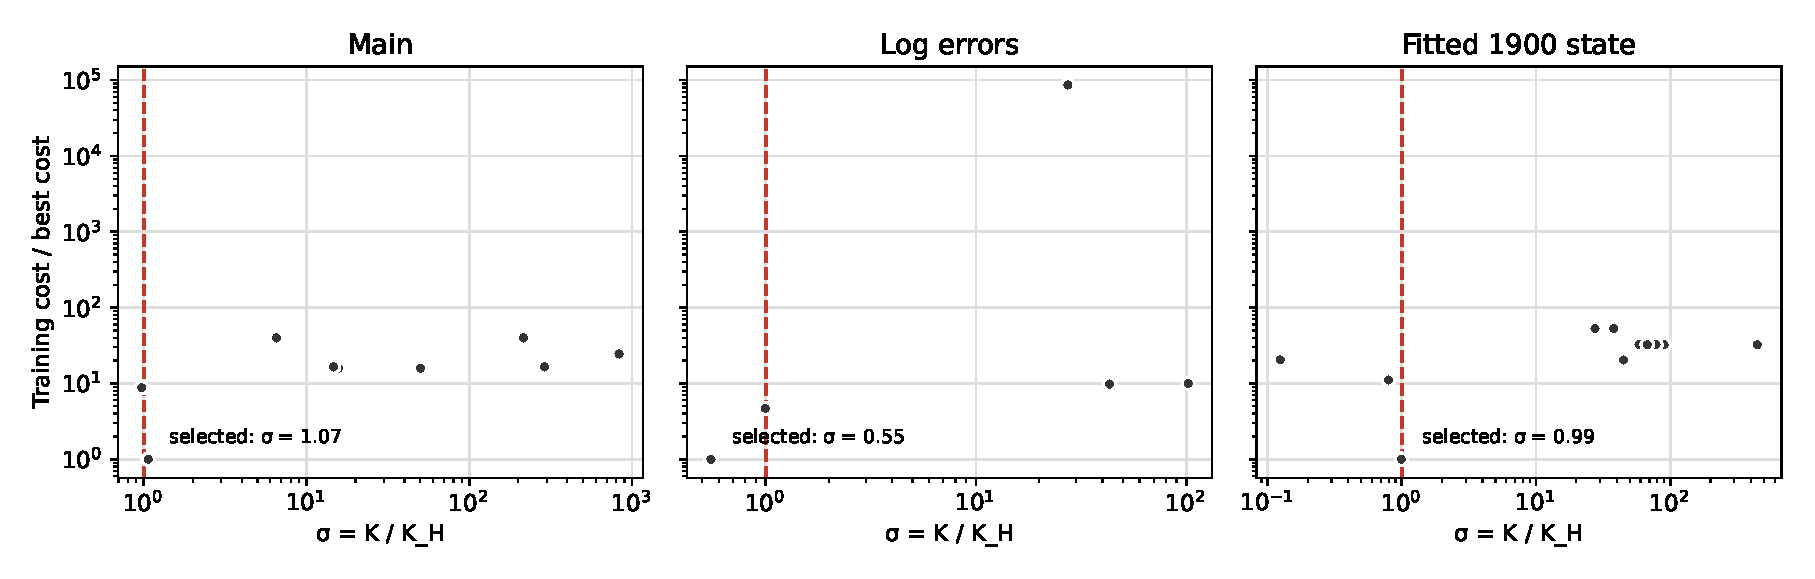
\includegraphics[width=\textwidth]{advay_baseline_sigma}
\caption{Training cost relative to the best, against $\sigma=K/K_H$, for every converged
start. The dashed line is the Hopf threshold $\sigma=1$. The best fits sit near $\sigma=1$,
on different sides depending on the variant.}\label{fig:advay-sigma}
\end{figure}

\subsection{Held-out evaluation, 1916--1920}\label{sec:advay-eval}

\paragraph{Protocol.} A scoring plan fixing the forecasts compared, the headline comparison,
the metrics and the interpretation rule was committed and published before the test file was
opened. All forecasts integrate frozen parameters from 1900 through 1920 with the shared
solver; nothing restarts from a test value, and no neural-network extrapolation is used.
For each species separately we report
$\mathrm{RMSE}=\big(\tfrac15\sum(\hat Y-Y)^2\big)^{1/2}$ and
$\mathrm{MAE}=\tfrac15\sum|\hat Y-Y|$ in thousands of pelts. With five test points a method
is called \emph{better} only if both its RMSE and MAE are smaller \emph{and} it is closer in
at least three of the five years; otherwise the methods are \emph{similar}. Two reference
forecasts use training data only: the 1915 value held constant (persistence) and the
1900--1915 mean. The headline comparison is the main least-squares fit against the
PINN-derived ODE forecast of the historical PINN study (seed chosen by training loss
before scoring). Every frozen forecast was checksum-verified, and the scores reproduce the
PINN study's own evaluation exactly.

\begin{table}[ht]
\centering
\input{tables/advay_heldout_metrics}
\caption{Held-out errors, 1916--1920, thousands of pelts.}\label{tab:advay-metrics}
\end{table}

\paragraph{Results.} (Table~\ref{tab:advay-metrics}, Figures~\ref{fig:advay-overlay}
and~\ref{fig:advay-metrics}.)
\begin{itemize}
\item \textbf{Both methods forecast the crash and recovery.} In the main variant both predict
the 1916--1920 lynx collapse and the hare recovery to within about 3--4 thousand pelts, far
better than persistence (lynx RMSE 37.2) or the training mean (lynx 10.6, hare 25.9). The
fitted dynamics carry real information about the next half-cycle.
\item \textbf{Headline: mixed and close.} Hare: similar (RMSE 3.07 least squares,
2.85 PINN; MAE 2.59 both). Lynx: least squares better (3.04 against 4.32, closer in all five
years); the PINN-derived lynx forecast falls to 3--5 thousand after 1918 where 9.7--10.1 were
observed.
\item \textbf{Sensitivity variants.} Least squares is better or similar in both. The log-error
PINN fit places the 1913 peaks about a year early and its forecast errors are large (hare RMSE 18.4).
\item \textbf{Why they differ.} Evaluated on $C$, the selected PINN parameters fit the
training years 1.9--3.4 times worse than the least-squares optimum, as expected for an
estimator that minimises a combined data and physics loss, and they cycle more strongly
($\sigma\approx1.35$). A better training fit did not give a better hare forecast in the main
variant. With five points, none of these differences is strong evidence.
\end{itemize}

\begin{figure}[ht]
\centering
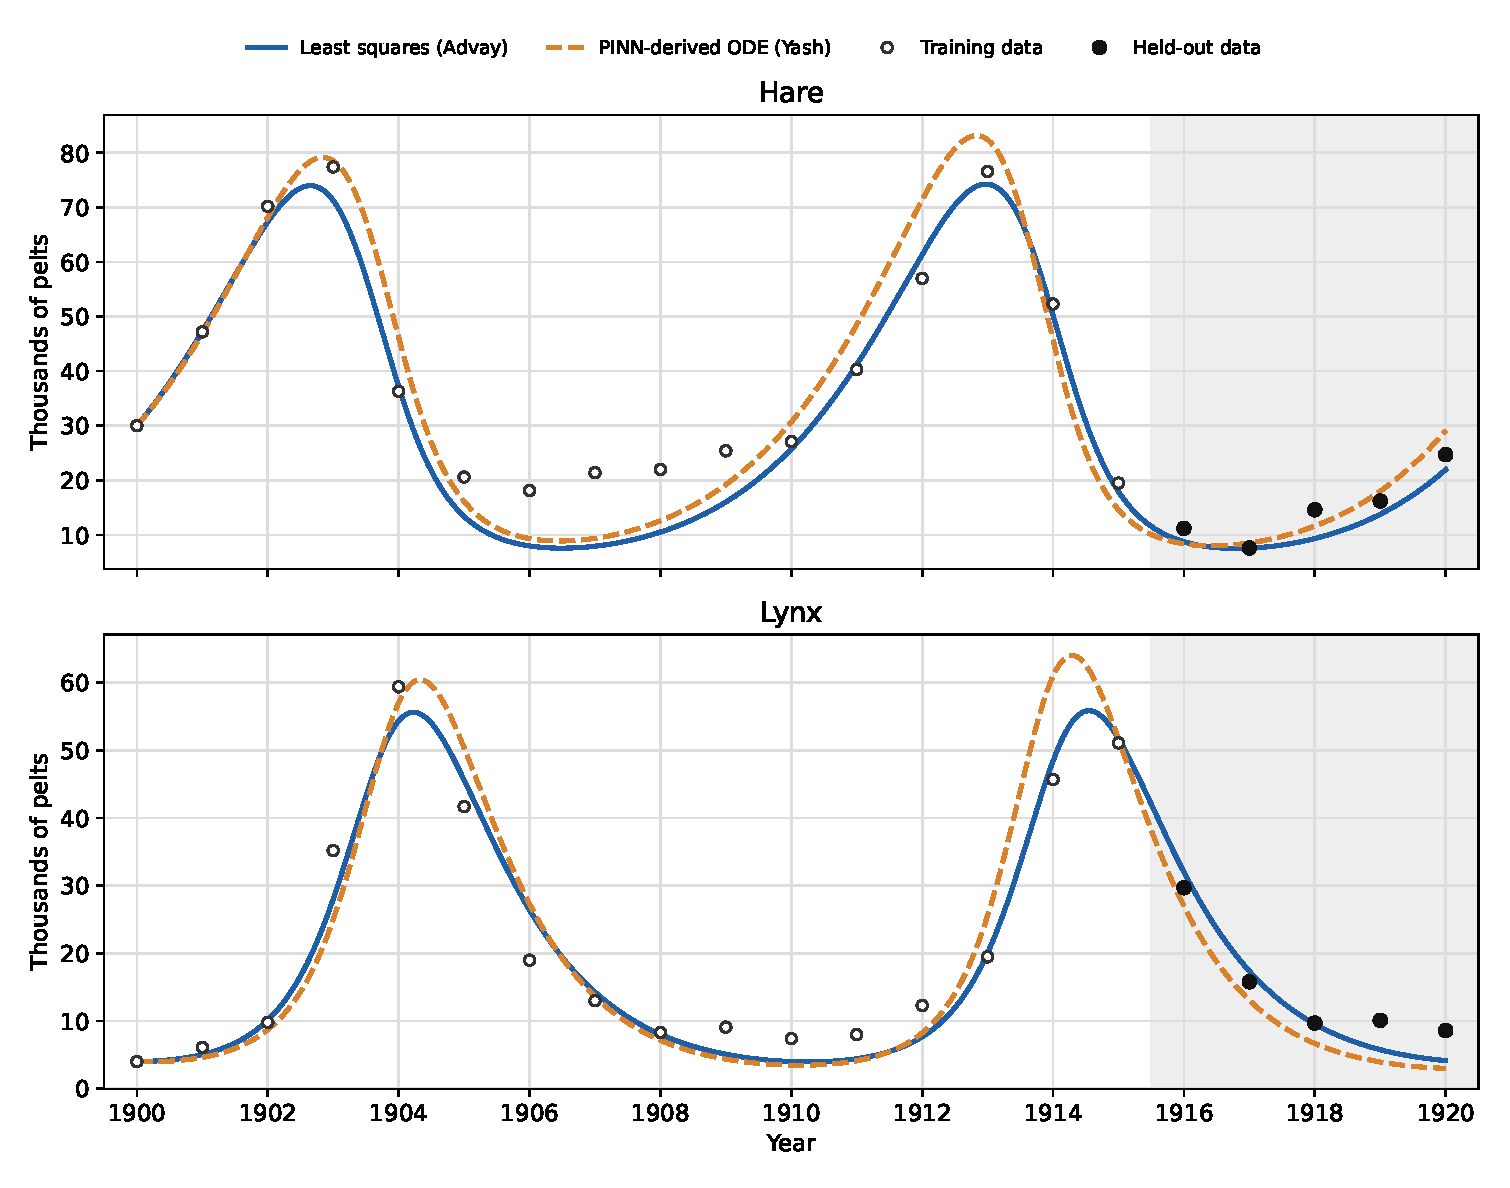
\includegraphics[width=0.9\textwidth]{advay_heldout_overlay}
\caption{Least-squares (solid) and PINN-derived (dashed) fits, main variant. Open circles:
training data; filled circles: held-out data (shaded). Both were fitted to 1900--1915 only
and integrated forward from 1900.}\label{fig:advay-overlay}
\end{figure}

\begin{figure}[ht]
\centering
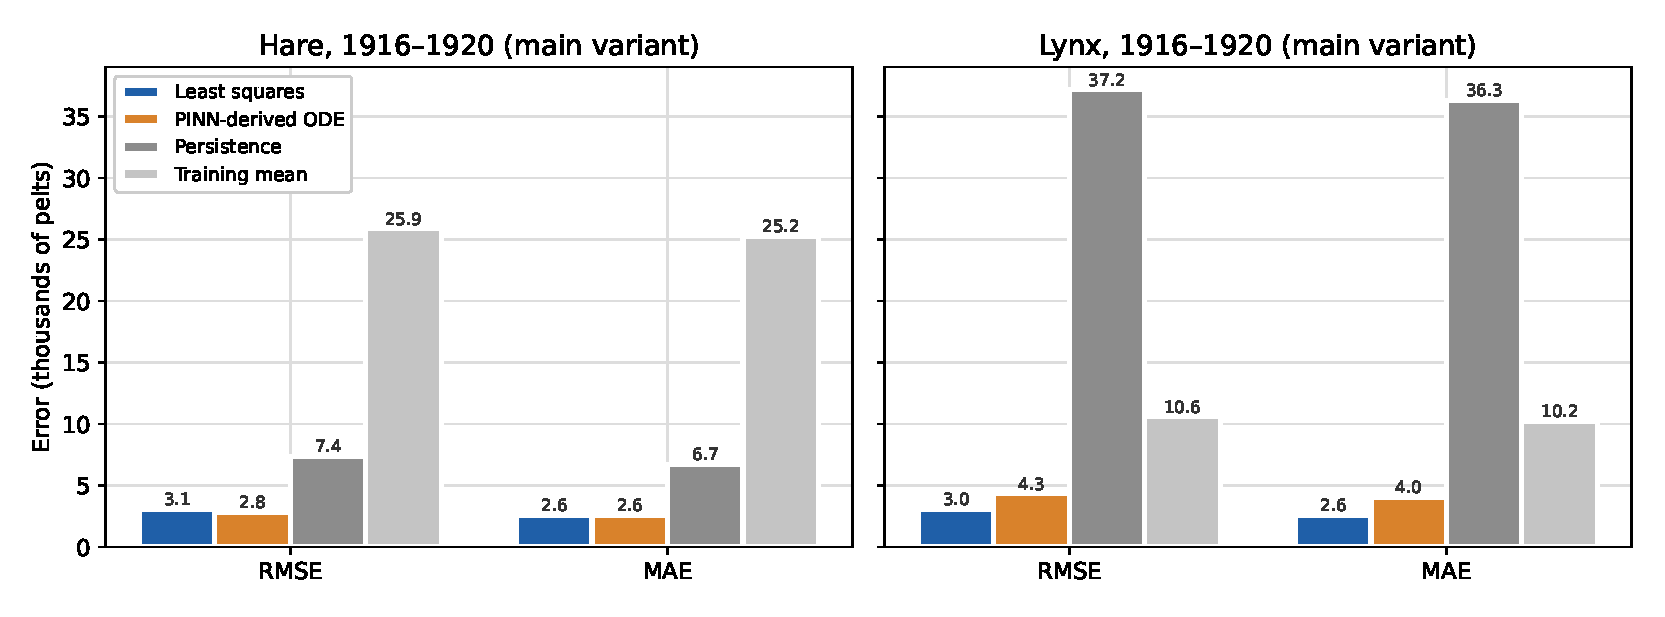
\includegraphics[width=\textwidth]{advay_heldout_metrics}
\caption{Held-out RMSE and MAE, main variant, with the persistence and training-mean
reference forecasts.}\label{fig:advay-metrics}
\end{figure}

\subsection{Limitations}\label{sec:advay-limits}

\begin{itemize}
\item \textbf{A very small test.} Five annual points, about half a cycle, beginning at the
1915 lynx peak. The comparison measures one crash and recovery, not long-run accuracy.
\item \textbf{Trade counts, not populations.} O1 assumes constant catchability; trapping
effort, prices and lynx behaviour almost certainly varied. Annual totals are treated as
point samples, a mismatch of up to a year in timing.
\item \textbf{Source uncertainty.} Two compilations of the same records disagree by more than
the forecast errors in some years; all results are conditional on the Stan series.
\item \textbf{Initial state.} The main analysis treats the noisy 1900 counts as exact. Fitting
them instead moves $\sigma$ from 1.07 to 0.99 and lowers the hare error.
\item \textbf{Identifiability.} $K$, $a$ and $b$ are individually poorly determined and $b$
(and $a$ in the main fit) lies on the box boundary, so their values depend on the chosen
bounds. A good curve fit is not evidence of uniquely recovered biological rates.
\item \textbf{Observation model.} Changing only the error model (additive to log) changes
$\sigma$ from 1.07 to 0.55 and the hare/lynx error balance, so the qualitative dynamics
inferred are sensitive to how the counts are assumed to be measured.
\item \textbf{Missing ecology.} A closed two-species, constant-parameter model omits
vegetation, other predators, weather, disease and spatial structure. Its success over
1916--1920 shows that it captures the dominant short-term feedback, not that it is complete.
\end{itemize}

\paragraph{Reproduction.} \texttt{scripts/advay\_data\_checks.py},
\texttt{advay\_make\_split.py}, \texttt{advay\_fit\_baseline.py --protocol v2},
\texttt{advay\_compare\_benchmark.py} and \texttt{advay\_score\_heldout.py} regenerate every
number and figure in this section; the declared protocols are in
\texttt{docs/advay\_baseline\_protocol.md} and \texttt{docs/advay\_scoring\_plan.md}.
   (standalone build: advay_main.tex)
% Figures: graphs/advay_*.{eps,pdf}; table: tables/advay_heldout_metrics.tex.
\section{Data, Least-Squares Baseline and Validation}\label{sec:advay}

This section states what the historical observations are, how they were prepared, how the
model was fitted to them by nonlinear least squares, and how well the fitted model forecasts
years it never saw. Every analysis choice that could be influenced by the held-out years was
written down and committed to the project repository before those years were opened.

\subsection{Data source and meaning}\label{sec:advay-data}

We use annual counts of snowshoe hare and Canadian lynx pelts traded by the Hudson's Bay
Company, 1900--1920, in thousands of pelts, as distributed with the Stan case study
\cite{carpenter2018}. Carpenter traces the numbers through Howard's lecture notes
\cite{howard2009} to a biology textbook; the original source is the Company's fur returns,
discussed by Hewitt \cite{hewitt1921}. The values are used unchanged
(\texttt{data/historical/pelts\_1900\_1920.csv}); the file's provenance, checksums and every
transformation (removing comment lines, reordering columns) are recorded alongside it.

These are \emph{trade counts}, not censuses. Trapping effort, fur prices, the number of
reporting posts and animal behaviour all affect them; Hewitt notes that hungry lynx are
easier to trap when hares are scarce. A second widely used compilation, the tsibbledata
\texttt{pelt} series \cite{tsibbledata_pelt}, differs noticeably over the same years
(Figure~\ref{fig:advay-sources}): the correlation between the two is 0.81 for lynx but only
0.32 for hare, and individual hare values differ by more than our forecast errors. We use
the Stan series because the project protocol names it, and treat the disagreement as a source
of uncertainty that no model in this report can remove.

\begin{figure}[ht]
\centering
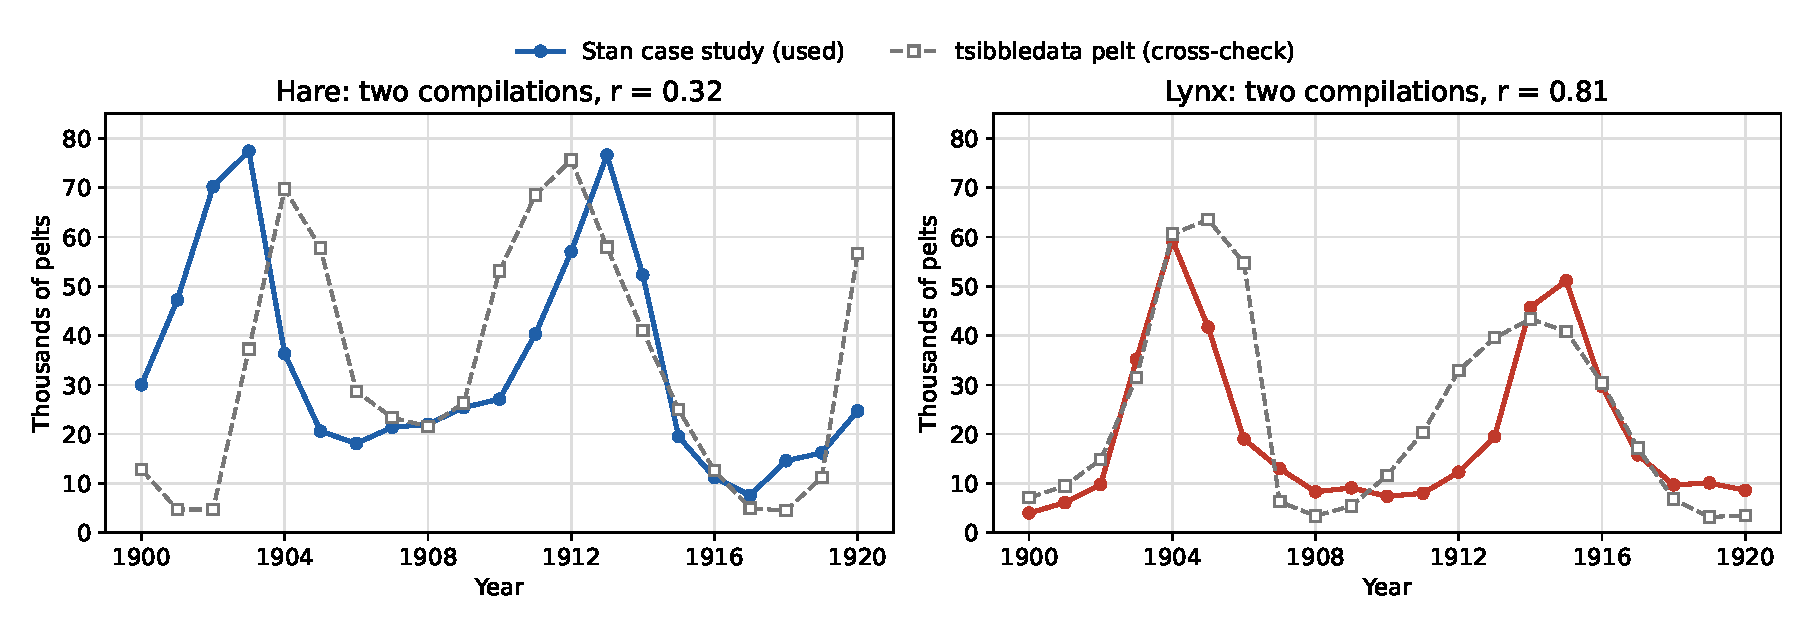
\includegraphics[width=\textwidth]{advay_source_comparison}
\caption{The Stan case-study series used here (solid) and the tsibbledata \texttt{pelt}
compilation (dashed) for 1900--1920. Both show two cycles, but yearly values differ,
especially for hare.}\label{fig:advay-sources}
\end{figure}

\paragraph{Observation model.} Following the agreed convention (assumption O1), pelt counts
are taken to be proportional to animal numbers with unknown constant factors, and the model
states are defined directly in pelt units:
\[
Y_{H,i}=H(t_i)+\varepsilon_{H,i},\qquad Y_{P,i}=P(t_i)+\varepsilon_{P,i},\qquad t_i=\mathrm{Year}_i-1900,
\]
with each annual total treated as a sample of the state at $t_i$. No observation scale factor
is fitted. Under O1, $r$, $m$ and the dimensionless groups of the model section are unchanged
by the unknown factors; $K$, $b$, $a$ and $e$ are \emph{effective} coefficients in pelt
units and are not interpreted as absolute biological quantities.

\subsection{Preparation and exploratory checks}\label{sec:advay-checks}

The 21 rows are consecutive, with no missing values, no zeros and no duplicates. The data
were split once into a training file (1900--1915, 16 rows) and a test file (1916--1920,
5 rows), with checksums recorded; all fitting code reads only the training file. Every
statistic below uses the training years only.

\begin{itemize}
\item \textbf{Cycles and lag.} Hare peaks in 1903 and 1913 (a ten-year spacing); lynx peaks
in 1904 and at the 1915 boundary. The correlation of $H(t)$ with $P(t+k)$ is largest at
$k=2$ years ($r=0.94$; $0.76$ at $k=1$). In the hare--lynx plane the data trace
counter-clockwise loops, as predator--prey models predict (Figure~\ref{fig:advay-raw}).
\item \textbf{Outliers.} None: robust $z$-scores of year-to-year log growth stay below 3
(largest 2.94, the 1903--1904 hare crash).
\item \textbf{Scale.} Training ranges are 18.1--77.4 (hare) and 4.0--59.4 (lynx). Hare counts
are about twice lynx counts, so residuals are divided by each species' training maximum
$(s_H,s_P)=(77.4,59.4)$ to weight the species equally. No log transform is used in the main
analysis; a log-residual fit is a declared sensitivity check.
\item \textbf{Split position.} Training ends exactly at the 1915 lynx peak, so the test years
are the following crash and the start of recovery: a turning point the fit never sees in
that cycle.
\end{itemize}

\begin{figure}[ht]
\centering
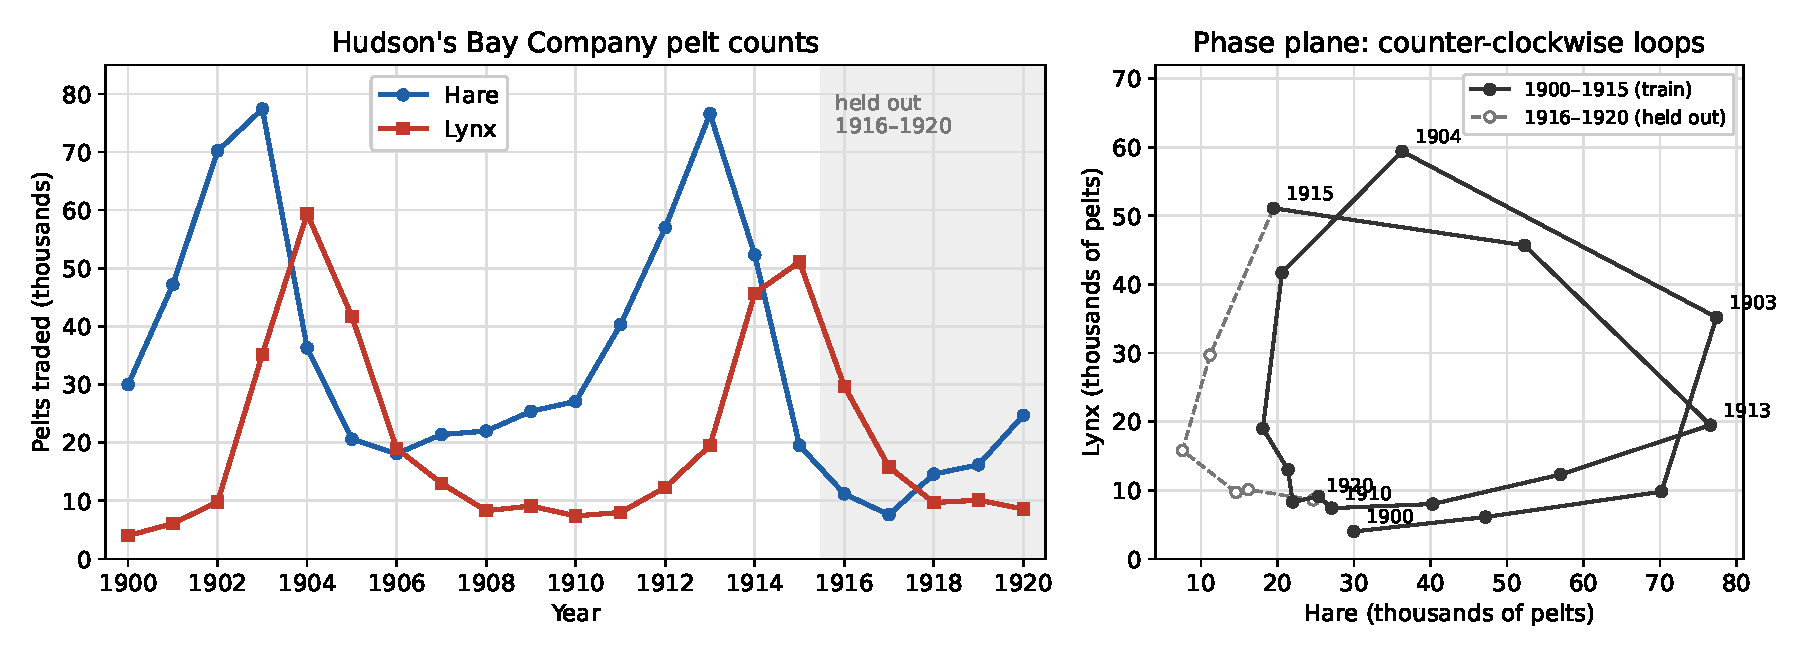
\includegraphics[width=\textwidth]{advay_raw_series}
\caption{Left: annual pelt counts, 1900--1920; the shaded band is held out. Right: the same
data in the hare--lynx plane (training solid, held-out dashed).}\label{fig:advay-raw}
\end{figure}

\subsection{Least-squares baseline}\label{sec:advay-ls}

\paragraph{Problem.} With $\theta=(r,K,a,b,e,m)$ and the shared RK45 solver (relative
tolerance $10^{-8}$, absolute $10^{-10}$, maximum step $0.1$ years), let $\hat H(t;\theta)$,
$\hat P(t;\theta)$ solve the model from the observed 1900 state $(30.0,4.0)$. The main
estimate minimises
\[
C(\theta)=\tfrac12\sum_{i=1900}^{1915}\Big[\big(\tfrac{\hat H(t_i;\theta)-Y_{H,i}}{s_H}\big)^2+
\big(\tfrac{\hat P(t_i;\theta)-Y_{P,i}}{s_P}\big)^2\Big]
\]
over the shared box bounds $r,m\in[0.05,3]$, $K\in[20,500]$, $a\in[0.05,10]$,
$b\in[0.5,300]$, $e\in[0.02,5]$. Two declared sensitivity variants change one assumption
each: \emph{log errors} replaces the scaled residuals by $\log\hat Y-\log Y$, and
\emph{fitted 1900 state} adds $(H_0,P_0)$ as unknowns within $[0.5,1.5]$ times the observed
values.

\paragraph{Method.} The bounded trust-region reflective algorithm (SciPy
\texttt{least\_squares}) is run in log-parameter space $x=\log\theta$, because the bounds
span up to a 600-fold range. Finite-difference steps of $10^{-4}$ in $x$ stay well above the
solver tolerance. The objective is multimodal, so each variant uses 80 starts: the shared
initial guess, 39 Latin-hypercube points uniform in $\log\theta$ and 39 uniform in $\theta$.
The fit with the lowest training cost is selected.

\paragraph{Protocol record.} The settings were committed before the first run. That run
(40 log-space starts) missed the best \emph{fitted 1900 state} fit, which an independent
benchmark had found at training cost $0.063$ against our $0.70$; evaluating our objective at
the benchmark's parameters gave $0.063$, so the code agreed and the start design was at
fault (the optimum sits near the upper bounds, which log-uniform starts rarely visit). The
uniform-scale starts were added as a declared amendment, judged on training cost alone and
before any test score of the baseline was computed. Both runs are kept.

\begin{table}[ht]
\centering
\begin{tabular}{lrrrrrrrl}
\toprule
Variant & $C$ & $r$ & $K$ & $a$ & $b$ & $e$ & $m$ & $\sigma=K/K_H$\\
\midrule
Main & 0.0845 & 0.647 & 382 & 10.0$^*$ & 300$^*$ & 0.967 & 0.857 & 1.07 (cycle)\\
Log errors & 0.903 & 0.520 & 197 & 7.17 & 300$^*$ & 1.80 & 1.15 & 0.55 (damped)\\
Fitted 1900 state & 0.0634 & 0.520 & 362 & 8.15 & 300$^*$ & 1.32 & 1.05 & 0.99 (damped)\\
\bottomrule
\end{tabular}
\caption{Least-squares estimates. $^*$ at the upper bound. Units: $r,m$ per year; $K,b$
thousands of hare pelts; $a,e$ effective pelt-unit coefficients. The fitted 1900 state in the
last variant is $(37.1,3.64)$.}\label{tab:advay-ls}
\end{table}

\paragraph{Results.} Table~\ref{tab:advay-ls} and Figure~\ref{fig:advay-fit} give the selected
fits. Three findings matter for interpretation.
\begin{enumerate}
\item \emph{The optimum is computationally well defined.} In every variant all starts within
1\% of the best cost (18, 42 and 16 of 80) found the same parameters to four significant
figures, and a separately written least-squares code by another team member reaches the same
optimum (training costs within $2\times10^{-7}$, forecasts within 0.002 thousand pelts).
\item \emph{The saturation of predation is not identified.} $b$ sits on its upper bound in
every variant. With $b$ about four times the largest hare count, $aH/(b+H)\approx(a/b)H$ over
the data: predation is nearly linear in hare abundance. In the linearised fit the
correlation between $\log a$ and $\log b$ is 0.998 and the approximate standard errors of
$\log K$, $\log a$, $\log b$ exceed 1 (a factor of three or more), whereas $r$, $e$, $m$ are
determined to about 10--40\%. Only the ratio $a/b\approx0.024$--$0.033$ is well determined.
Because the optimum lies on the boundary, its location depends on the chosen box.
\item \emph{Limit cycle or damped oscillation is not decided.} Using the Hopf threshold
$K_H=b(ea+m)/(ea-m)$ from the stability analysis, $\sigma$ is 1.07 for the main fit (just past the threshold),
0.99 with a fitted 1900 state (just below) and 0.55 with log errors. All three reproduce the
observed timing equally well (hare peaks fitted at 1902.5--1902.8 and 1912.6--1913.0, lynx
1.6 years later, period about ten years). Two cycles of data cannot distinguish a stable
limit cycle from a slowly damped oscillation (Figure~\ref{fig:advay-sigma}).
\end{enumerate}

\begin{figure}[ht]
\centering
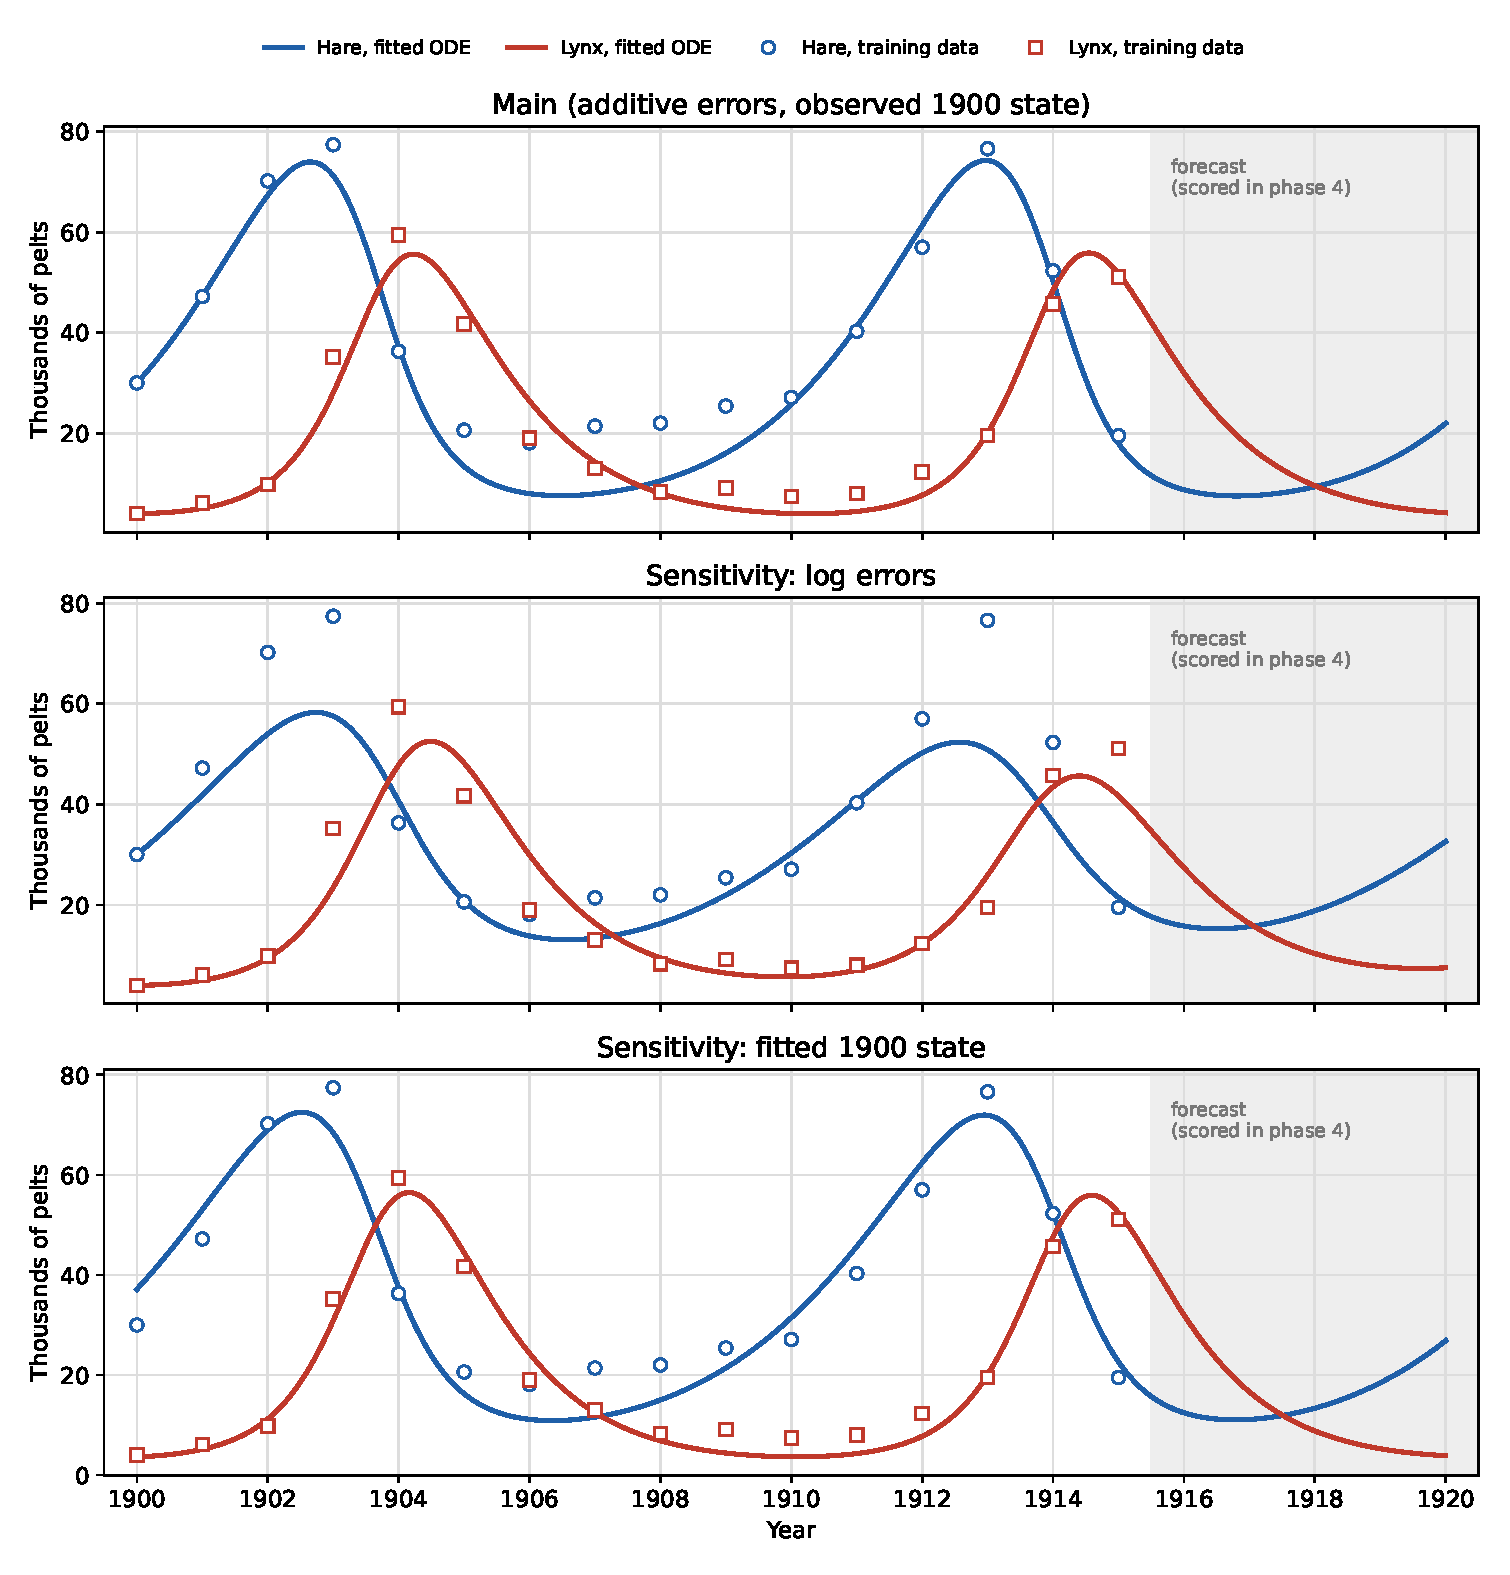
\includegraphics[width=0.9\textwidth]{advay_baseline_fit}
\caption{Least-squares fits to the 1900--1915 pelt counts (markers) and their continuation
through 1920 (shaded, held out) for the main analysis and both sensitivity variants.}
\label{fig:advay-fit}
\end{figure}

\begin{figure}[ht]
\centering
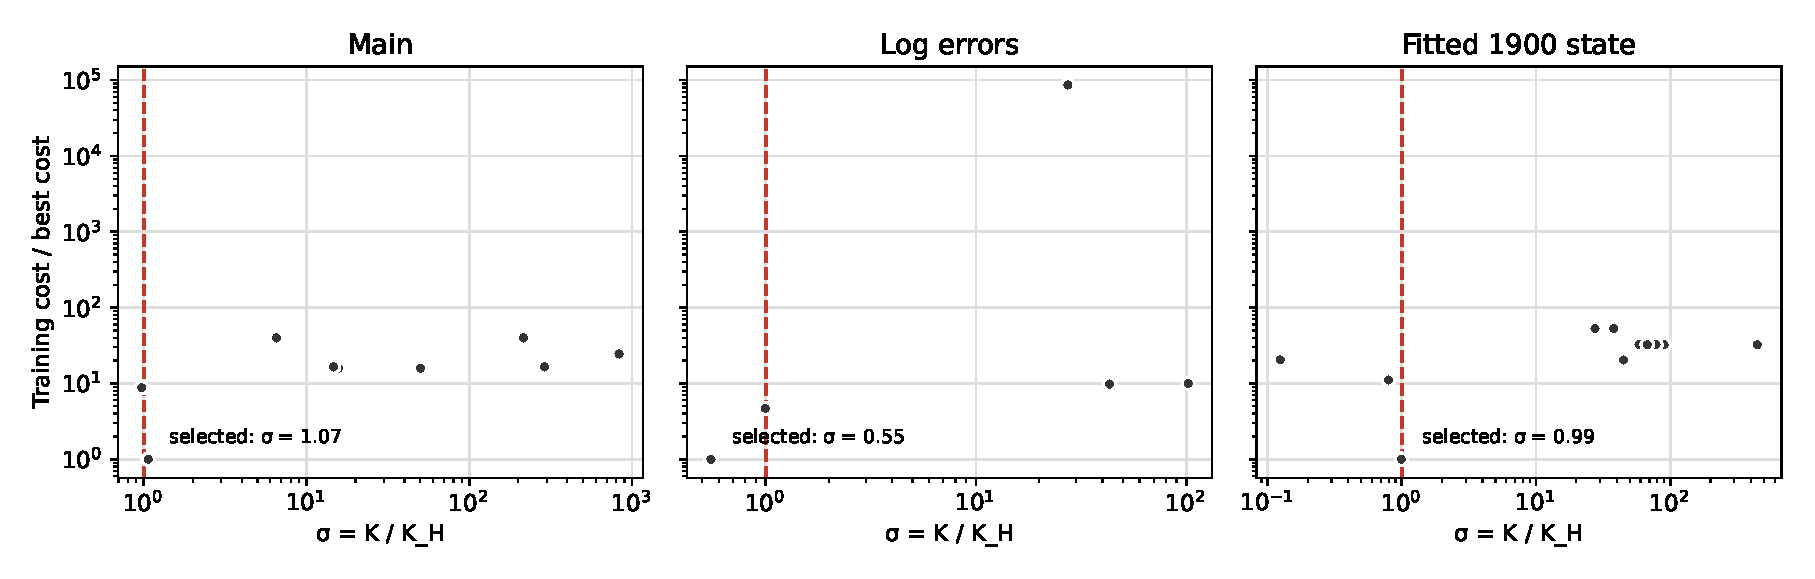
\includegraphics[width=\textwidth]{advay_baseline_sigma}
\caption{Training cost relative to the best, against $\sigma=K/K_H$, for every converged
start. The dashed line is the Hopf threshold $\sigma=1$. The best fits sit near $\sigma=1$,
on different sides depending on the variant.}\label{fig:advay-sigma}
\end{figure}

\subsection{Held-out evaluation, 1916--1920}\label{sec:advay-eval}

\paragraph{Protocol.} A scoring plan fixing the forecasts compared, the headline comparison,
the metrics and the interpretation rule was committed and published before the test file was
opened. All forecasts integrate frozen parameters from 1900 through 1920 with the shared
solver; nothing restarts from a test value, and no neural-network extrapolation is used.
For each species separately we report
$\mathrm{RMSE}=\big(\tfrac15\sum(\hat Y-Y)^2\big)^{1/2}$ and
$\mathrm{MAE}=\tfrac15\sum|\hat Y-Y|$ in thousands of pelts. With five test points a method
is called \emph{better} only if both its RMSE and MAE are smaller \emph{and} it is closer in
at least three of the five years; otherwise the methods are \emph{similar}. Two reference
forecasts use training data only: the 1915 value held constant (persistence) and the
1900--1915 mean. The headline comparison is the main least-squares fit against the
PINN-derived ODE forecast of the historical PINN study (seed chosen by training loss
before scoring). Every frozen forecast was checksum-verified, and the scores reproduce the
PINN study's own evaluation exactly.

\begin{table}[ht]
\centering
\begin{tabular}{llrrrr}
\hline
Variant & Method & Hare RMSE & Hare MAE & Lynx RMSE & Lynx MAE \\
\hline
Main (headline) & Least squares & 3.07 & 2.59 & 3.04 & 2.56 \\
 & PINN-derived ODE (seed17) & 2.85 & 2.59 & 4.32 & 4.05 \\
Log errors & Least squares & 6.87 & 6.63 & 1.60 & 1.38 \\
 & PINN-derived ODE (seed29) & 18.35 & 14.29 & 10.03 & 8.97 \\
Fitted 1900 state & Least squares & 2.25 & 2.08 & 3.24 & 2.71 \\
 & PINN-derived ODE (seed17) & 3.69 & 3.06 & 4.70 & 4.53 \\
\hline
Reference & Persistence (1915 value) & 7.38 & 6.72 & 37.16 & 36.32 \\
Reference & Training mean & 25.87 & 25.23 & 10.58 & 10.21 \\
\hline
\end{tabular}

\caption{Held-out errors, 1916--1920, thousands of pelts.}\label{tab:advay-metrics}
\end{table}

\paragraph{Results.} (Table~\ref{tab:advay-metrics}, Figures~\ref{fig:advay-overlay}
and~\ref{fig:advay-metrics}.)
\begin{itemize}
\item \textbf{Both methods forecast the crash and recovery.} In the main variant both predict
the 1916--1920 lynx collapse and the hare recovery to within about 3--4 thousand pelts, far
better than persistence (lynx RMSE 37.2) or the training mean (lynx 10.6, hare 25.9). The
fitted dynamics carry real information about the next half-cycle.
\item \textbf{Headline: mixed and close.} Hare: similar (RMSE 3.07 least squares,
2.85 PINN; MAE 2.59 both). Lynx: least squares better (3.04 against 4.32, closer in all five
years); the PINN-derived lynx forecast falls to 3--5 thousand after 1918 where 9.7--10.1 were
observed.
\item \textbf{Sensitivity variants.} Least squares is better or similar in both. The log-error
PINN fit places the 1913 peaks about a year early and its forecast errors are large (hare RMSE 18.4).
\item \textbf{Why they differ.} Evaluated on $C$, the selected PINN parameters fit the
training years 1.9--3.4 times worse than the least-squares optimum, as expected for an
estimator that minimises a combined data and physics loss, and they cycle more strongly
($\sigma\approx1.35$). A better training fit did not give a better hare forecast in the main
variant. With five points, none of these differences is strong evidence.
\end{itemize}

\begin{figure}[ht]
\centering
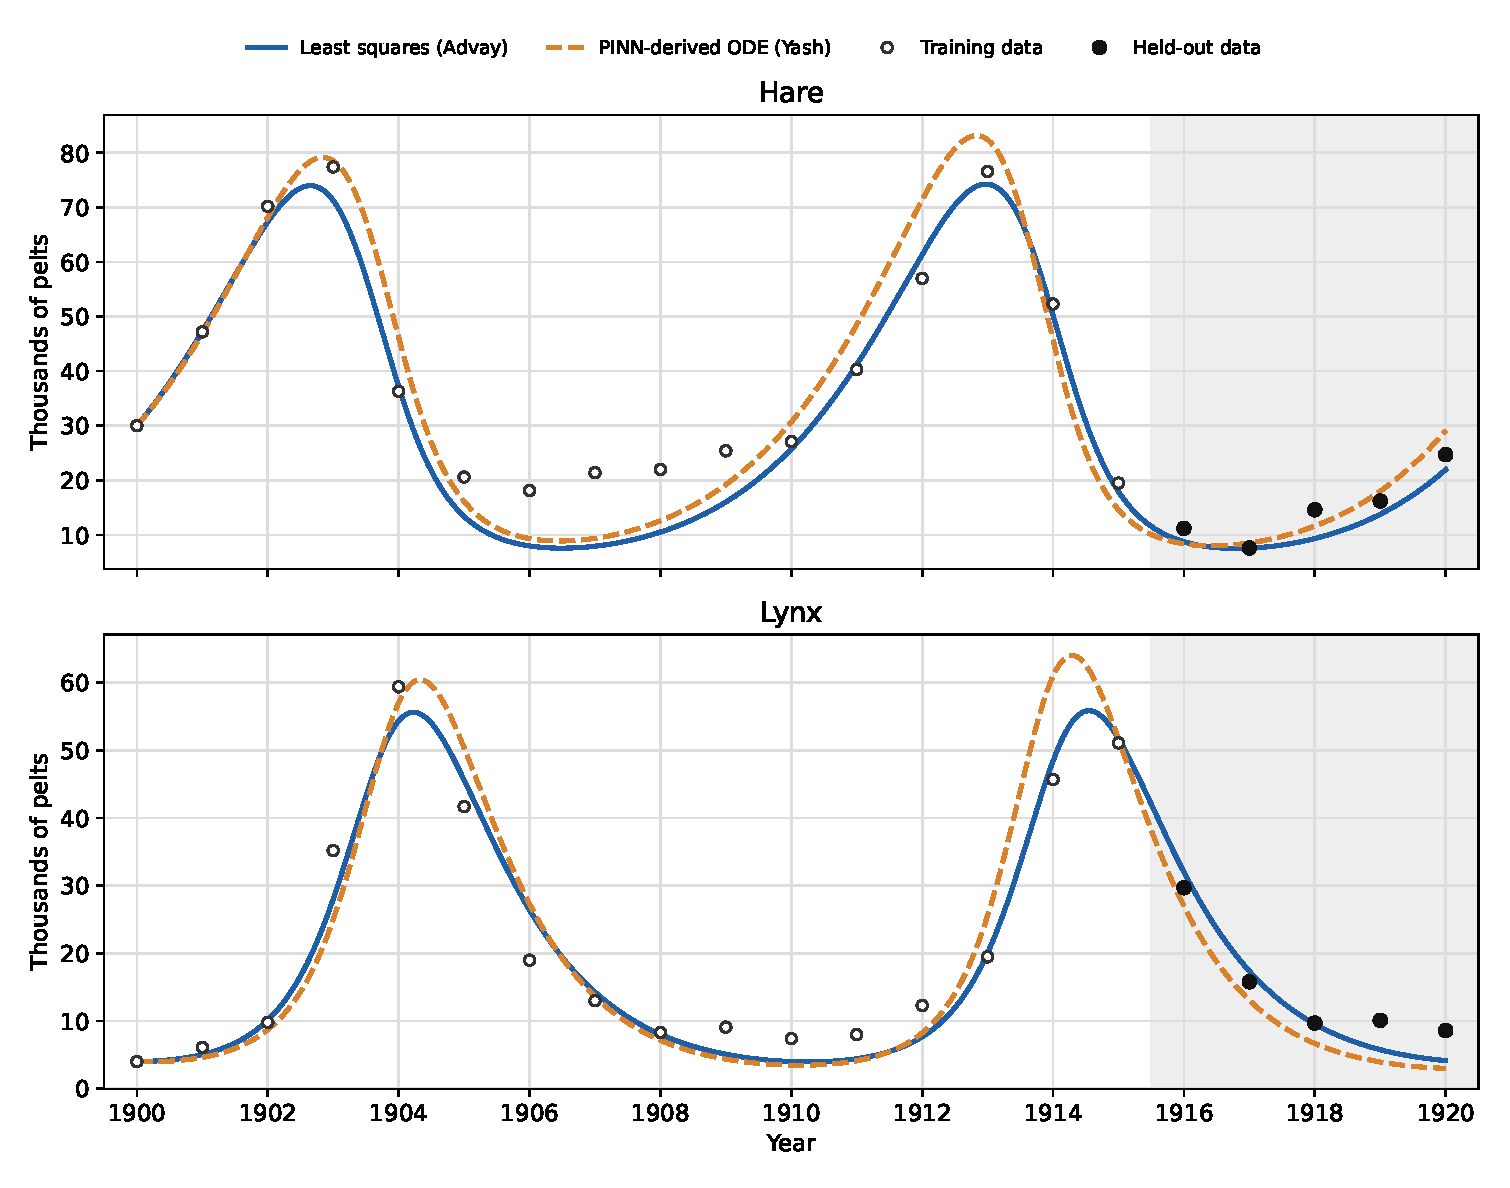
\includegraphics[width=0.9\textwidth]{advay_heldout_overlay}
\caption{Least-squares (solid) and PINN-derived (dashed) fits, main variant. Open circles:
training data; filled circles: held-out data (shaded). Both were fitted to 1900--1915 only
and integrated forward from 1900.}\label{fig:advay-overlay}
\end{figure}

\begin{figure}[ht]
\centering
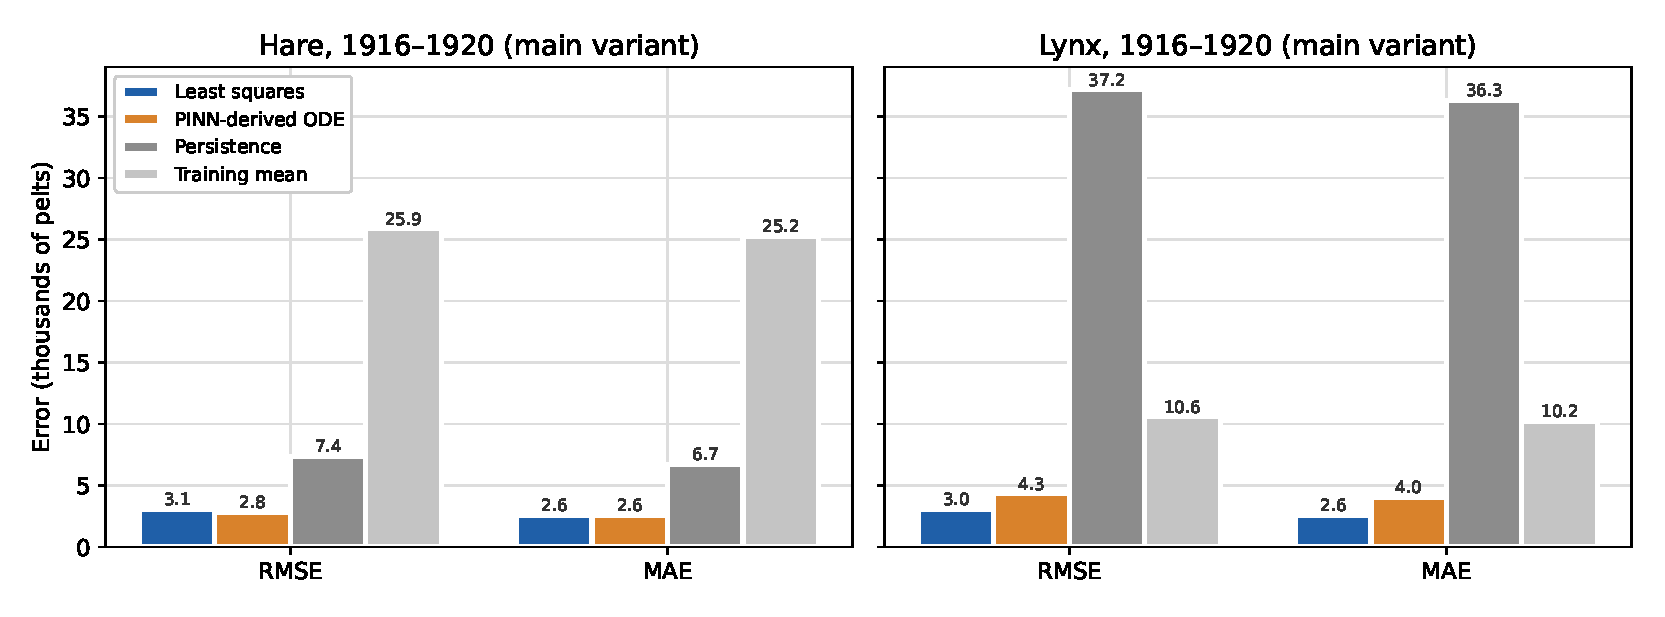
\includegraphics[width=\textwidth]{advay_heldout_metrics}
\caption{Held-out RMSE and MAE, main variant, with the persistence and training-mean
reference forecasts.}\label{fig:advay-metrics}
\end{figure}

\subsection{Limitations}\label{sec:advay-limits}

\begin{itemize}
\item \textbf{A very small test.} Five annual points, about half a cycle, beginning at the
1915 lynx peak. The comparison measures one crash and recovery, not long-run accuracy.
\item \textbf{Trade counts, not populations.} O1 assumes constant catchability; trapping
effort, prices and lynx behaviour almost certainly varied. Annual totals are treated as
point samples, a mismatch of up to a year in timing.
\item \textbf{Source uncertainty.} Two compilations of the same records disagree by more than
the forecast errors in some years; all results are conditional on the Stan series.
\item \textbf{Initial state.} The main analysis treats the noisy 1900 counts as exact. Fitting
them instead moves $\sigma$ from 1.07 to 0.99 and lowers the hare error.
\item \textbf{Identifiability.} $K$, $a$ and $b$ are individually poorly determined and $b$
(and $a$ in the main fit) lies on the box boundary, so their values depend on the chosen
bounds. A good curve fit is not evidence of uniquely recovered biological rates.
\item \textbf{Observation model.} Changing only the error model (additive to log) changes
$\sigma$ from 1.07 to 0.55 and the hare/lynx error balance, so the qualitative dynamics
inferred are sensitive to how the counts are assumed to be measured.
\item \textbf{Missing ecology.} A closed two-species, constant-parameter model omits
vegetation, other predators, weather, disease and spatial structure. Its success over
1916--1920 shows that it captures the dominant short-term feedback, not that it is complete.
\end{itemize}

\paragraph{Reproduction.} \texttt{scripts/advay\_data\_checks.py},
\texttt{advay\_make\_split.py}, \texttt{advay\_fit\_baseline.py --protocol v2},
\texttt{advay\_compare\_benchmark.py} and \texttt{advay\_score\_heldout.py} regenerate every
number and figure in this section; the declared protocols are in
\texttt{docs/advay\_baseline\_protocol.md} and \texttt{docs/advay\_scoring\_plan.md}.
   (standalone build: advay_main.tex)
% Figures: graphs/advay_*.{eps,pdf}; table: tables/advay_heldout_metrics.tex.
\section{Data, Least-Squares Baseline and Validation}\label{sec:advay}

This section states what the historical observations are, how they were prepared, how the
model was fitted to them by nonlinear least squares, and how well the fitted model forecasts
years it never saw. Every analysis choice that could be influenced by the held-out years was
written down and committed to the project repository before those years were opened.

\subsection{Data source and meaning}\label{sec:advay-data}

We use annual counts of snowshoe hare and Canadian lynx pelts traded by the Hudson's Bay
Company, 1900--1920, in thousands of pelts, as distributed with the Stan case study
\cite{carpenter2018}. Carpenter traces the numbers through Howard's lecture notes
\cite{howard2009} to a biology textbook; the original source is the Company's fur returns,
discussed by Hewitt \cite{hewitt1921}. The values are used unchanged
(\texttt{data/historical/pelts\_1900\_1920.csv}); the file's provenance, checksums and every
transformation (removing comment lines, reordering columns) are recorded alongside it.

These are \emph{trade counts}, not censuses. Trapping effort, fur prices, the number of
reporting posts and animal behaviour all affect them; Hewitt notes that hungry lynx are
easier to trap when hares are scarce. A second widely used compilation, the tsibbledata
\texttt{pelt} series \cite{tsibbledata_pelt}, differs noticeably over the same years
(Figure~\ref{fig:advay-sources}): the correlation between the two is 0.81 for lynx but only
0.32 for hare, and individual hare values differ by more than our forecast errors. We use
the Stan series because the project protocol names it, and treat the disagreement as a source
of uncertainty that no model in this report can remove.

\begin{figure}[ht]
\centering
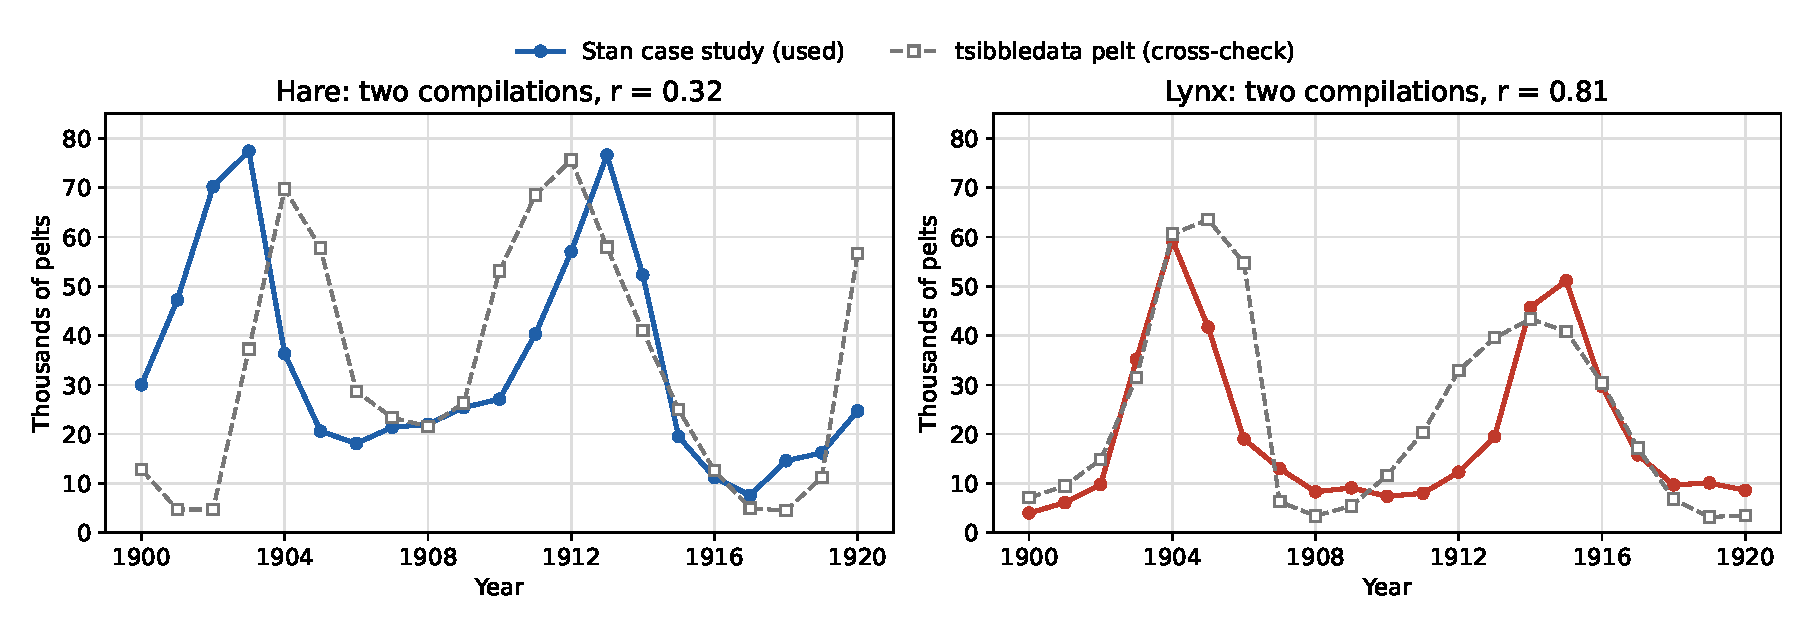
\includegraphics[width=\textwidth]{advay_source_comparison}
\caption{The Stan case-study series used here (solid) and the tsibbledata \texttt{pelt}
compilation (dashed) for 1900--1920. Both show two cycles, but yearly values differ,
especially for hare.}\label{fig:advay-sources}
\end{figure}

\paragraph{Observation model.} Following the agreed convention (assumption O1), pelt counts
are taken to be proportional to animal numbers with unknown constant factors, and the model
states are defined directly in pelt units:
\[
Y_{H,i}=H(t_i)+\varepsilon_{H,i},\qquad Y_{P,i}=P(t_i)+\varepsilon_{P,i},\qquad t_i=\mathrm{Year}_i-1900,
\]
with each annual total treated as a sample of the state at $t_i$. No observation scale factor
is fitted. Under O1, $r$, $m$ and the dimensionless groups of the model section are unchanged
by the unknown factors; $K$, $b$, $a$ and $e$ are \emph{effective} coefficients in pelt
units and are not interpreted as absolute biological quantities.

\subsection{Preparation and exploratory checks}\label{sec:advay-checks}

The 21 rows are consecutive, with no missing values, no zeros and no duplicates. The data
were split once into a training file (1900--1915, 16 rows) and a test file (1916--1920,
5 rows), with checksums recorded; all fitting code reads only the training file. Every
statistic below uses the training years only.

\begin{itemize}
\item \textbf{Cycles and lag.} Hare peaks in 1903 and 1913 (a ten-year spacing); lynx peaks
in 1904 and at the 1915 boundary. The correlation of $H(t)$ with $P(t+k)$ is largest at
$k=2$ years ($r=0.94$; $0.76$ at $k=1$). In the hare--lynx plane the data trace
counter-clockwise loops, as predator--prey models predict (Figure~\ref{fig:advay-raw}).
\item \textbf{Outliers.} None: robust $z$-scores of year-to-year log growth stay below 3
(largest 2.94, the 1903--1904 hare crash).
\item \textbf{Scale.} Training ranges are 18.1--77.4 (hare) and 4.0--59.4 (lynx). Hare counts
are about twice lynx counts, so residuals are divided by each species' training maximum
$(s_H,s_P)=(77.4,59.4)$ to weight the species equally. No log transform is used in the main
analysis; a log-residual fit is a declared sensitivity check.
\item \textbf{Split position.} Training ends exactly at the 1915 lynx peak, so the test years
are the following crash and the start of recovery: a turning point the fit never sees in
that cycle.
\end{itemize}

\begin{figure}[ht]
\centering
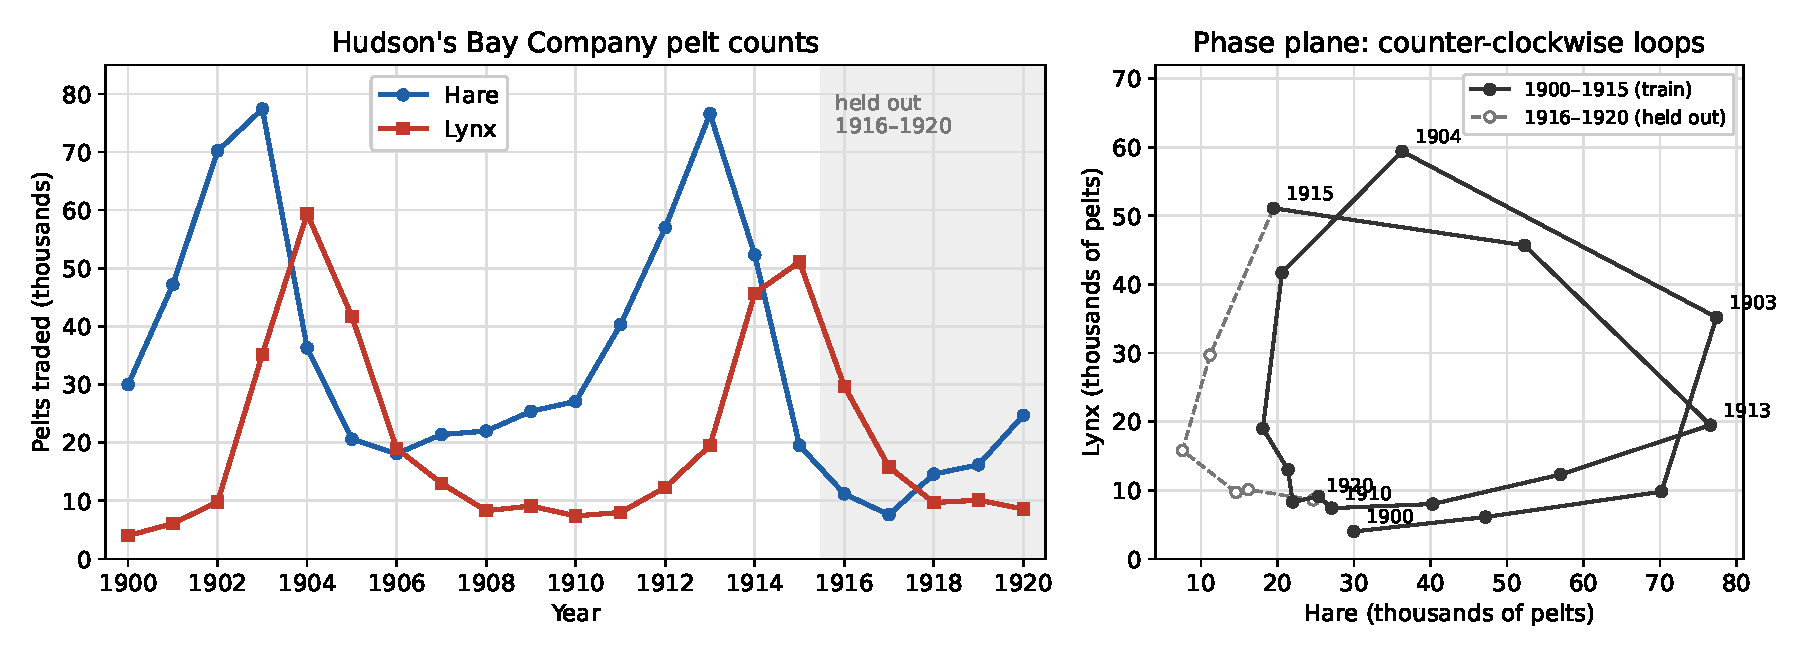
\includegraphics[width=\textwidth]{advay_raw_series}
\caption{Left: annual pelt counts, 1900--1920; the shaded band is held out. Right: the same
data in the hare--lynx plane (training solid, held-out dashed).}\label{fig:advay-raw}
\end{figure}

\subsection{Least-squares baseline}\label{sec:advay-ls}

\paragraph{Problem.} With $\theta=(r,K,a,b,e,m)$ and the shared RK45 solver (relative
tolerance $10^{-8}$, absolute $10^{-10}$, maximum step $0.1$ years), let $\hat H(t;\theta)$,
$\hat P(t;\theta)$ solve the model from the observed 1900 state $(30.0,4.0)$. The main
estimate minimises
\[
C(\theta)=\tfrac12\sum_{i=1900}^{1915}\Big[\big(\tfrac{\hat H(t_i;\theta)-Y_{H,i}}{s_H}\big)^2+
\big(\tfrac{\hat P(t_i;\theta)-Y_{P,i}}{s_P}\big)^2\Big]
\]
over the shared box bounds $r,m\in[0.05,3]$, $K\in[20,500]$, $a\in[0.05,10]$,
$b\in[0.5,300]$, $e\in[0.02,5]$. Two declared sensitivity variants change one assumption
each: \emph{log errors} replaces the scaled residuals by $\log\hat Y-\log Y$, and
\emph{fitted 1900 state} adds $(H_0,P_0)$ as unknowns within $[0.5,1.5]$ times the observed
values.

\paragraph{Method.} The bounded trust-region reflective algorithm (SciPy
\texttt{least\_squares}) is run in log-parameter space $x=\log\theta$, because the bounds
span up to a 600-fold range. Finite-difference steps of $10^{-4}$ in $x$ stay well above the
solver tolerance. The objective is multimodal, so each variant uses 80 starts: the shared
initial guess, 39 Latin-hypercube points uniform in $\log\theta$ and 39 uniform in $\theta$.
The fit with the lowest training cost is selected.

\paragraph{Protocol record.} The settings were committed before the first run. That run
(40 log-space starts) missed the best \emph{fitted 1900 state} fit, which an independent
benchmark had found at training cost $0.063$ against our $0.70$; evaluating our objective at
the benchmark's parameters gave $0.063$, so the code agreed and the start design was at
fault (the optimum sits near the upper bounds, which log-uniform starts rarely visit). The
uniform-scale starts were added as a declared amendment, judged on training cost alone and
before any test score of the baseline was computed. Both runs are kept.

\begin{table}[ht]
\centering
\begin{tabular}{lrrrrrrrl}
\toprule
Variant & $C$ & $r$ & $K$ & $a$ & $b$ & $e$ & $m$ & $\sigma=K/K_H$\\
\midrule
Main & 0.0845 & 0.647 & 382 & 10.0$^*$ & 300$^*$ & 0.967 & 0.857 & 1.07 (cycle)\\
Log errors & 0.903 & 0.520 & 197 & 7.17 & 300$^*$ & 1.80 & 1.15 & 0.55 (damped)\\
Fitted 1900 state & 0.0634 & 0.520 & 362 & 8.15 & 300$^*$ & 1.32 & 1.05 & 0.99 (damped)\\
\bottomrule
\end{tabular}
\caption{Least-squares estimates. $^*$ at the upper bound. Units: $r,m$ per year; $K,b$
thousands of hare pelts; $a,e$ effective pelt-unit coefficients. The fitted 1900 state in the
last variant is $(37.1,3.64)$.}\label{tab:advay-ls}
\end{table}

\paragraph{Results.} Table~\ref{tab:advay-ls} and Figure~\ref{fig:advay-fit} give the selected
fits. Three findings matter for interpretation.
\begin{enumerate}
\item \emph{The optimum is computationally well defined.} In every variant all starts within
1\% of the best cost (18, 42 and 16 of 80) found the same parameters to four significant
figures, and a separately written least-squares code by another team member reaches the same
optimum (training costs within $2\times10^{-7}$, forecasts within 0.002 thousand pelts).
\item \emph{The saturation of predation is not identified.} $b$ sits on its upper bound in
every variant. With $b$ about four times the largest hare count, $aH/(b+H)\approx(a/b)H$ over
the data: predation is nearly linear in hare abundance. In the linearised fit the
correlation between $\log a$ and $\log b$ is 0.998 and the approximate standard errors of
$\log K$, $\log a$, $\log b$ exceed 1 (a factor of three or more), whereas $r$, $e$, $m$ are
determined to about 10--40\%. Only the ratio $a/b\approx0.024$--$0.033$ is well determined.
Because the optimum lies on the boundary, its location depends on the chosen box.
\item \emph{Limit cycle or damped oscillation is not decided.} Using the Hopf threshold
$K_H=b(ea+m)/(ea-m)$ from the stability analysis, $\sigma$ is 1.07 for the main fit (just past the threshold),
0.99 with a fitted 1900 state (just below) and 0.55 with log errors. All three reproduce the
observed timing equally well (hare peaks fitted at 1902.5--1902.8 and 1912.6--1913.0, lynx
1.6 years later, period about ten years). Two cycles of data cannot distinguish a stable
limit cycle from a slowly damped oscillation (Figure~\ref{fig:advay-sigma}).
\end{enumerate}

\begin{figure}[ht]
\centering
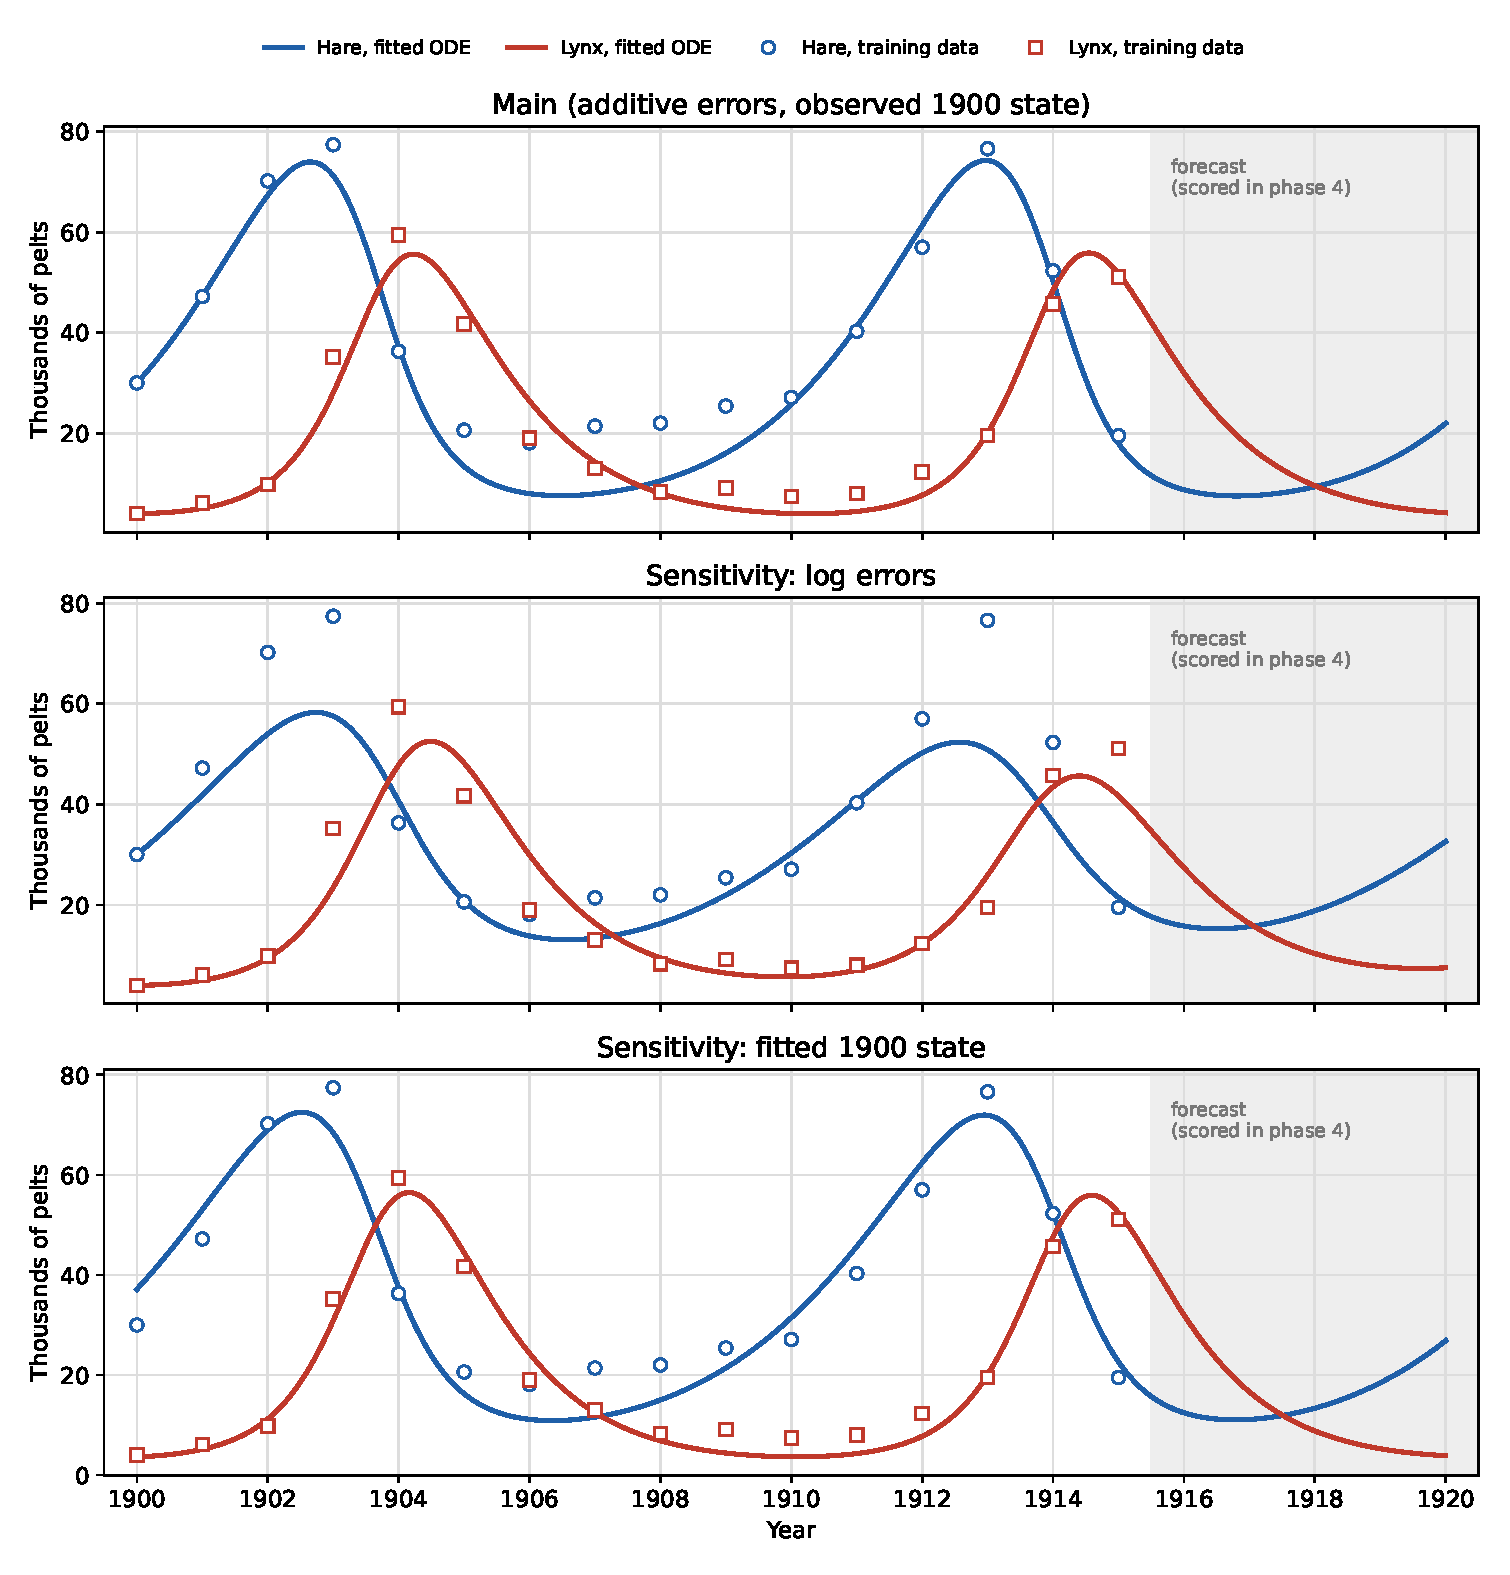
\includegraphics[width=0.9\textwidth]{advay_baseline_fit}
\caption{Least-squares fits to the 1900--1915 pelt counts (markers) and their continuation
through 1920 (shaded, held out) for the main analysis and both sensitivity variants.}
\label{fig:advay-fit}
\end{figure}

\begin{figure}[ht]
\centering
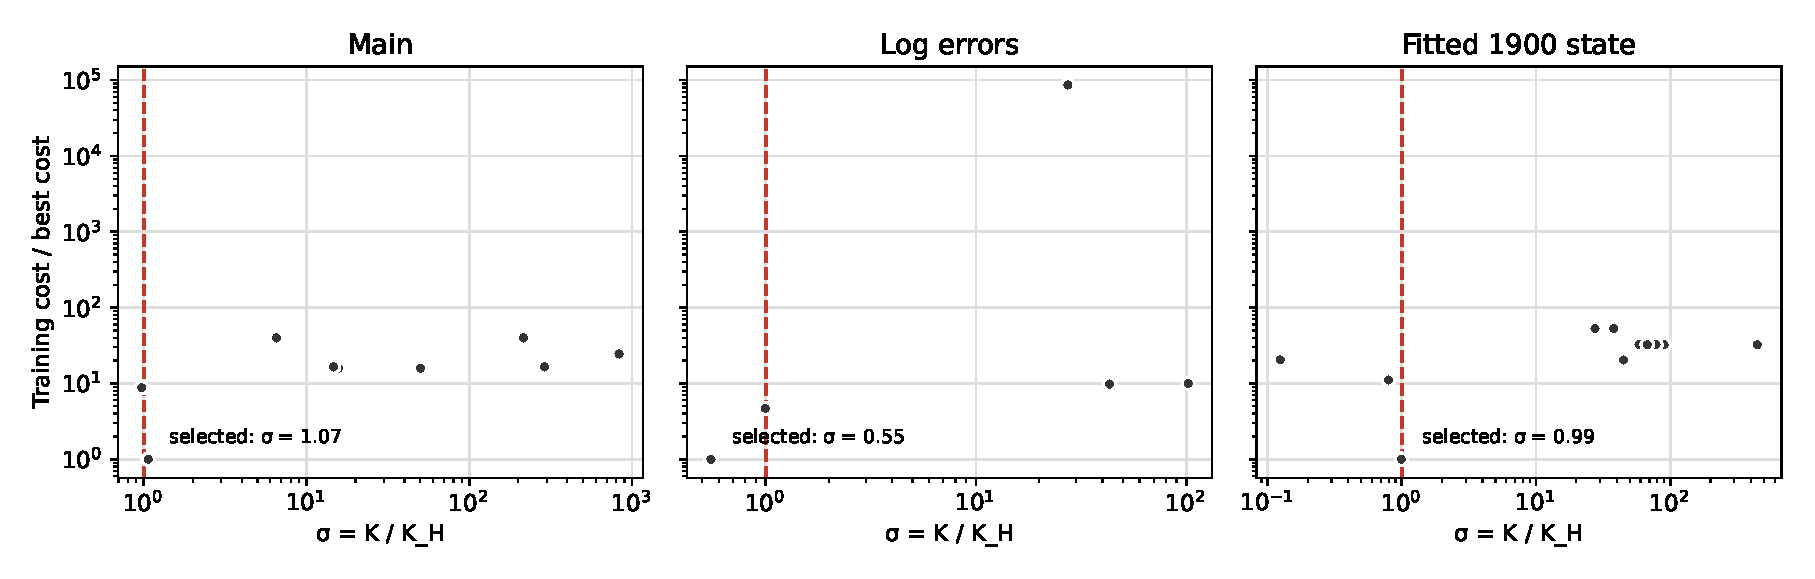
\includegraphics[width=\textwidth]{advay_baseline_sigma}
\caption{Training cost relative to the best, against $\sigma=K/K_H$, for every converged
start. The dashed line is the Hopf threshold $\sigma=1$. The best fits sit near $\sigma=1$,
on different sides depending on the variant.}\label{fig:advay-sigma}
\end{figure}

\subsection{Held-out evaluation, 1916--1920}\label{sec:advay-eval}

\paragraph{Protocol.} A scoring plan fixing the forecasts compared, the headline comparison,
the metrics and the interpretation rule was committed and published before the test file was
opened. All forecasts integrate frozen parameters from 1900 through 1920 with the shared
solver; nothing restarts from a test value, and no neural-network extrapolation is used.
For each species separately we report
$\mathrm{RMSE}=\big(\tfrac15\sum(\hat Y-Y)^2\big)^{1/2}$ and
$\mathrm{MAE}=\tfrac15\sum|\hat Y-Y|$ in thousands of pelts. With five test points a method
is called \emph{better} only if both its RMSE and MAE are smaller \emph{and} it is closer in
at least three of the five years; otherwise the methods are \emph{similar}. Two reference
forecasts use training data only: the 1915 value held constant (persistence) and the
1900--1915 mean. The headline comparison is the main least-squares fit against the
PINN-derived ODE forecast of the historical PINN study (seed chosen by training loss
before scoring). Every frozen forecast was checksum-verified, and the scores reproduce the
PINN study's own evaluation exactly.

\begin{table}[ht]
\centering
\begin{tabular}{llrrrr}
\hline
Variant & Method & Hare RMSE & Hare MAE & Lynx RMSE & Lynx MAE \\
\hline
Main (headline) & Least squares & 3.07 & 2.59 & 3.04 & 2.56 \\
 & PINN-derived ODE (seed17) & 2.85 & 2.59 & 4.32 & 4.05 \\
Log errors & Least squares & 6.87 & 6.63 & 1.60 & 1.38 \\
 & PINN-derived ODE (seed29) & 18.35 & 14.29 & 10.03 & 8.97 \\
Fitted 1900 state & Least squares & 2.25 & 2.08 & 3.24 & 2.71 \\
 & PINN-derived ODE (seed17) & 3.69 & 3.06 & 4.70 & 4.53 \\
\hline
Reference & Persistence (1915 value) & 7.38 & 6.72 & 37.16 & 36.32 \\
Reference & Training mean & 25.87 & 25.23 & 10.58 & 10.21 \\
\hline
\end{tabular}

\caption{Held-out errors, 1916--1920, thousands of pelts.}\label{tab:advay-metrics}
\end{table}

\paragraph{Results.} (Table~\ref{tab:advay-metrics}, Figures~\ref{fig:advay-overlay}
and~\ref{fig:advay-metrics}.)
\begin{itemize}
\item \textbf{Both methods forecast the crash and recovery.} In the main variant both predict
the 1916--1920 lynx collapse and the hare recovery to within about 3--4 thousand pelts, far
better than persistence (lynx RMSE 37.2) or the training mean (lynx 10.6, hare 25.9). The
fitted dynamics carry real information about the next half-cycle.
\item \textbf{Headline: mixed and close.} Hare: similar (RMSE 3.07 least squares,
2.85 PINN; MAE 2.59 both). Lynx: least squares better (3.04 against 4.32, closer in all five
years); the PINN-derived lynx forecast falls to 3--5 thousand after 1918 where 9.7--10.1 were
observed.
\item \textbf{Sensitivity variants.} Least squares is better or similar in both. The log-error
PINN fit places the 1913 peaks about a year early and its forecast errors are large (hare RMSE 18.4).
\item \textbf{Why they differ.} Evaluated on $C$, the selected PINN parameters fit the
training years 1.9--3.4 times worse than the least-squares optimum, as expected for an
estimator that minimises a combined data and physics loss, and they cycle more strongly
($\sigma\approx1.35$). A better training fit did not give a better hare forecast in the main
variant. With five points, none of these differences is strong evidence.
\end{itemize}

\begin{figure}[ht]
\centering
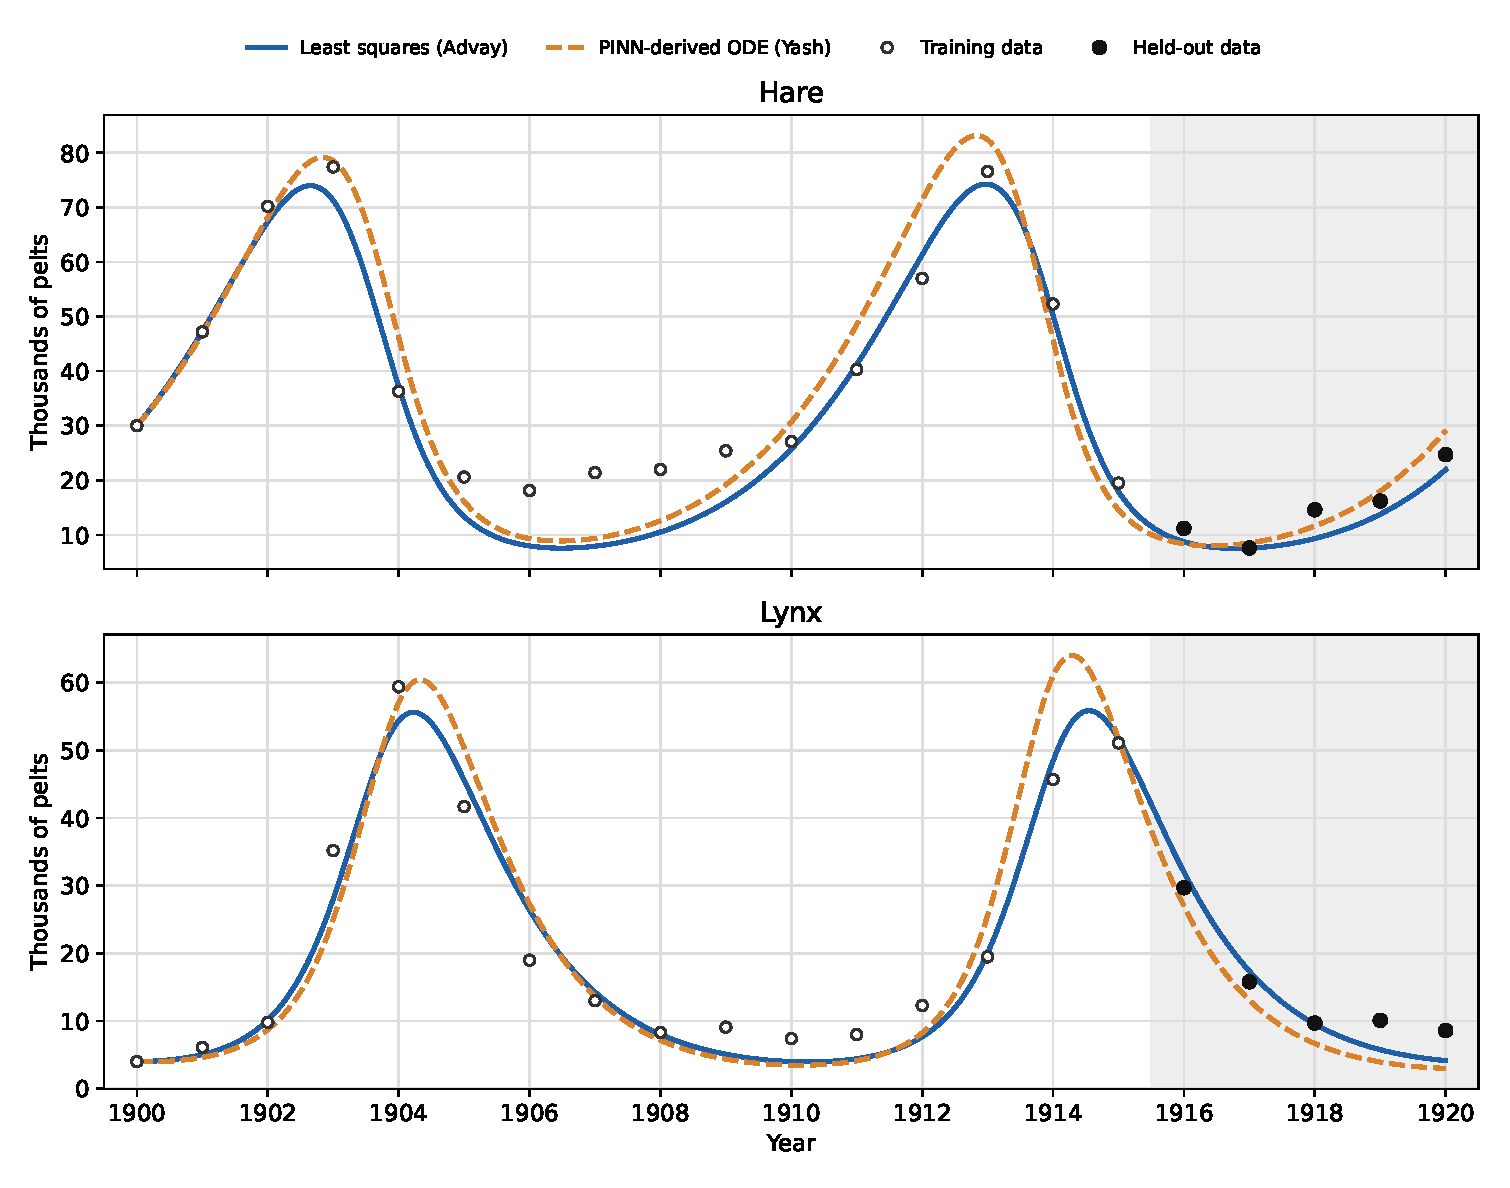
\includegraphics[width=0.9\textwidth]{advay_heldout_overlay}
\caption{Least-squares (solid) and PINN-derived (dashed) fits, main variant. Open circles:
training data; filled circles: held-out data (shaded). Both were fitted to 1900--1915 only
and integrated forward from 1900.}\label{fig:advay-overlay}
\end{figure}

\begin{figure}[ht]
\centering
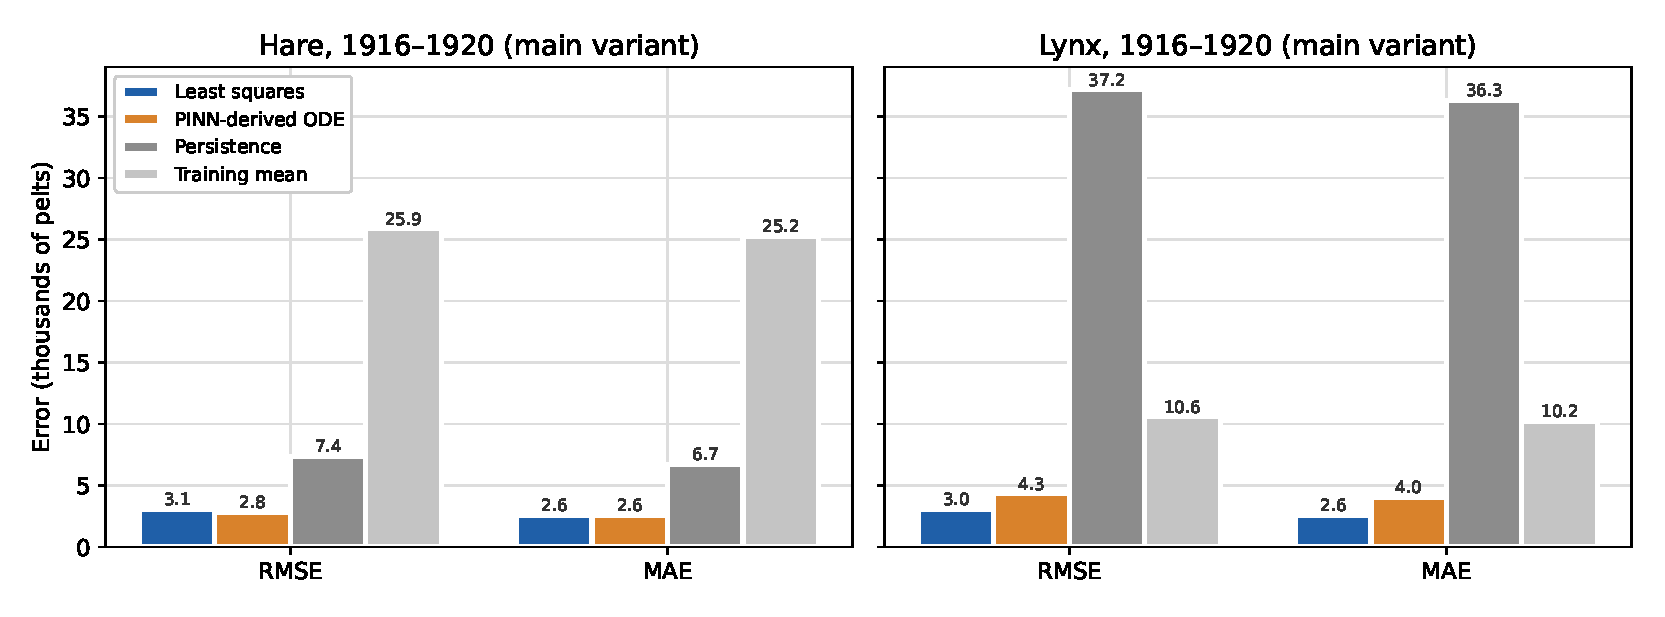
\includegraphics[width=\textwidth]{advay_heldout_metrics}
\caption{Held-out RMSE and MAE, main variant, with the persistence and training-mean
reference forecasts.}\label{fig:advay-metrics}
\end{figure}

\subsection{Limitations}\label{sec:advay-limits}

\begin{itemize}
\item \textbf{A very small test.} Five annual points, about half a cycle, beginning at the
1915 lynx peak. The comparison measures one crash and recovery, not long-run accuracy.
\item \textbf{Trade counts, not populations.} O1 assumes constant catchability; trapping
effort, prices and lynx behaviour almost certainly varied. Annual totals are treated as
point samples, a mismatch of up to a year in timing.
\item \textbf{Source uncertainty.} Two compilations of the same records disagree by more than
the forecast errors in some years; all results are conditional on the Stan series.
\item \textbf{Initial state.} The main analysis treats the noisy 1900 counts as exact. Fitting
them instead moves $\sigma$ from 1.07 to 0.99 and lowers the hare error.
\item \textbf{Identifiability.} $K$, $a$ and $b$ are individually poorly determined and $b$
(and $a$ in the main fit) lies on the box boundary, so their values depend on the chosen
bounds. A good curve fit is not evidence of uniquely recovered biological rates.
\item \textbf{Observation model.} Changing only the error model (additive to log) changes
$\sigma$ from 1.07 to 0.55 and the hare/lynx error balance, so the qualitative dynamics
inferred are sensitive to how the counts are assumed to be measured.
\item \textbf{Missing ecology.} A closed two-species, constant-parameter model omits
vegetation, other predators, weather, disease and spatial structure. Its success over
1916--1920 shows that it captures the dominant short-term feedback, not that it is complete.
\end{itemize}

\paragraph{Reproduction.} \texttt{scripts/advay\_data\_checks.py},
\texttt{advay\_make\_split.py}, \texttt{advay\_fit\_baseline.py --protocol v2},
\texttt{advay\_compare\_benchmark.py} and \texttt{advay\_score\_heldout.py} regenerate every
number and figure in this section; the declared protocols are in
\texttt{docs/advay\_baseline\_protocol.md} and \texttt{docs/advay\_scoring\_plan.md}.
\clearpage
\section{Controlled synthetic validation}
The separate synthetic study tests implementation recovery with known parameters and
3\% observation noise. Across three annual-data seeds, the largest relative error in
the three inferred rates is below 0.36\%. K, b and e are correctly fixed at generating
values for that controlled test; historical fitting instead estimates all six.
This favorable recovery experiment is not evidence of historical parameter accuracy.
Its complete program, recovery tables, residuals and sensitivity runs remain in
\path{notebooks/yash_pinn.ipynb} and \path{results/synthetic/}.
\ReportGraphEPS[width=\linewidth]{parameter_recovery.eps}
\paragraph{Reproduction and acknowledgement.}
Run the combined notebook \path{notebooks/group_project.ipynb} from a fresh Python
environment using the supplied requirements. Full expensive experiment drivers and
individual notebooks remain alongside the frozen evidence. All report plots have EPS
sources and vector PDF companions. Per-person AI assistance and actual manual-review
records are in \path{docs/ai_acknowledgement.md} and Arnav's contribution folder.
Each member remains responsible for understanding and explaining their own work.
\clearpage\bibliographystyle{plain}\bibliography{group_references}
\end{document}
